\RequirePackage{lineno}
\documentclass{cmspaper}
\usepackage{graphicx}
\usepackage{amsmath}
\usepackage{amssymb}
\usepackage{subfigure}
\usepackage{multirow}
% % useful definitions

% processes
\def\dyee {\ensuremath{Z/\gamma^*\to ee}}
\def\dymm {\ensuremath{Z/\gamma^*\to\mu\mu}}
\def\dytt {\ensuremath{Z/\gamma^*\to\tau\tau}}
\def\zee {\ensuremath{Z\to ee}}
\def\zmm {\ensuremath{Z\to\mu\mu}}
\def\ztt {\ensuremath{Z\to\tau\tau}}
\def\ttbar {\ensuremath{t\bar{t}}}
\def\wwll {\ensuremath{WW\to l^+l^-}}
\def\wwlulu{\ensuremath{WW\to l^+\nu l^-\bar{\nu}}}
\def\ww {\ensuremath{WW}}
\def\hww {\ensuremath{H\to WW}}
\def\wz{\ensuremath{WZ}}
\def\zz{\ensuremath{ZZ}}
\def\wgamma{\ensuremath{W\gamma}}
\def\wjets{\ensuremath{W+}jets} 
\def\tw{\ensuremath{tW}} 
\def\singletopt{\ensuremath{t} ($t$-chan)} 
\def\singletops{\ensuremath{t} ($s$-chan)} 
\def\all{all}
\def\ee{\ensuremath{ee}}
\def\emu{\ensuremath{e\mu}}
\def\mm{\ensuremath{\mu\mu}}

%units
\newcommand{\TeV}{\ensuremath{\mathrm{Te\kern -0.1em V}}}
\newcommand{\GeV}{\ensuremath{\mathrm{Ge\kern -0.1em V}}}

%others
\def\pt{\ensuremath{p_T}}
\def\ipb{pb\ensuremath{^{-1}}}
\def\ifb{fb\ensuremath{^{-1}}}
\def\et{\ensuremath{E_T}}
\def\met{\ensuremath{E\!\!\!\!/_T}}
\def\fBrem{\ensuremath{f_{\rm brem}}}
\def\pin{\ensuremath{p_{\rm in}}}
\def\pout{\ensuremath{p_{\rm out}}}

\newcommand{\CLs}{\ensuremath{CL_\mathrm{s}}}
\newcommand{\CLb}{\ensuremath{CL_\mathrm{b}}}
\newcommand{\CLsb}{\ensuremath{CL_\mathrm{s+b}}}

\newcommand{\GeV}{\ensuremath{\mathrm{Ge\kern -0.1em V}}}
\newcommand{\TeV}{\ensuremath{\mathrm{Te\kern -0.1em V}}}
\newcommand{\TeVcc}{\ensuremath{\,\mathrm{Te\kern -0.1em V\!/c}^2}}
\newcommand{\GeVcc}{\ensuremath{\,\mathrm{Ge\kern -0.1em V\!/c}^2}}
\newcommand{\MeVcc}{\ensuremath{\,\mathrm{Me\kern -0.1em V\!/c}^2}}
\newcommand{\GeVc}{\ensuremath{\mathrm{Ge\kern -0.1em V}\!/c}}
\newcommand{\nanob}{\mbox{{\rm ~nb}~}}
\newcommand{\fb}{\ensuremath{\mathrm{fb}}}
\newcommand{\pb}{\ensuremath{\mathrm{pb}}}
\newcommand{\ifb}{\ensuremath{\mathrm{fb^{-1}}}}
\newcommand{\ipb}{\ensuremath{\mathrm{pb^{-1}}}}
\newcommand{\grad}{\ensuremath{^{\circ}}}
%
% Special user made math symbols
%
\newcommand{\lsim}{\raisebox{-1.5mm}{$\:\stackrel{\textstyle{<}}{\textstyle{\sim}}\:$}}
\newcommand{\gsim}{\raisebox{-1.5mm}{$\:\stackrel{\textstyle{>}}{\textstyle{\sim}}\:$}}

% particles

\newcommand{\pipm}{\ensuremath{\pi^{\pm}}}
\newcommand{\pizero}{\ensuremath{\pi^{0}}}
\newcommand{\Hi}{\ensuremath{\mathrm{H}}}
\newcommand{\W}{\ensuremath{\mathrm{W}}}
\newcommand{\Wjets}{\ensuremath{\mathrm{W+jets}}}
\newcommand{\Zjets}{\ensuremath{\mathrm{Z+jets}}}
\newcommand{\Wt}{\ensuremath{\mathrm{Wt}}}
\newcommand{\Wstar}{\ensuremath{\mathrm{W}^{*}}}
\newcommand{\Wparenthesisstar}{\ensuremath{\mathrm{W}^{(*)}}}
\newcommand{\WW}{\ensuremath{\W^+\W^-}}
\newcommand{\Z}{\ensuremath{\mathrm{Z}}}
\newcommand{\Zstar}{\ensuremath{\mathrm{Z}^{*}}}
\newcommand{\Astar}{\ensuremath{\mathrm{\gamma}^{*}}}
\newcommand{\ZZ}{\ensuremath{\Z\Z}}
\newcommand{\WZ}{\ensuremath{\W\Z}}
\newcommand{\Wgstar}{\ensuremath{\W\Astar}}
\newcommand{\E}{\ensuremath{\mathrm{e}}}
\newcommand{\Ep}{\ensuremath{\mathrm{e}^{+}}}
\newcommand{\Em}{\ensuremath{\mathrm{e}^{-}}}
\newcommand{\Epm}{\ensuremath{\mathrm{e}^{\pm}}}
\newcommand{\Emp}{\ensuremath{\mathrm{e}^{\mp}}}
\newcommand{\M}{\ensuremath{\mu}}
\newcommand{\Mp}{\ensuremath{\mu^{+}}}
\newcommand{\Mm}{\ensuremath{\mu^{-}}}
\newcommand{\Mpm}{\ensuremath{\mu^{\pm}}}
\newcommand{\Mmp}{\ensuremath{\mu^{\mp}}}
\newcommand{\Tau}{\ensuremath{\tau}}
\newcommand{\Nu}{\ensuremath{\nu}}
\newcommand{\Nubar}{\ensuremath{\bar{\nu}}}
\newcommand{\Lep}{\ensuremath{\ell}}
\newcommand{\Lepp}{\ensuremath{\ell^{+}}}
\newcommand{\Lepm}{\ensuremath{\ell^{-}}}
\newcommand{\Lprime}{\ensuremath{\Lep^{\prime}}}
\newcommand{\Prot}{\ensuremath{\mathrm{p}}}
\newcommand{\Pbar}{\ensuremath{\bar{\mathrm{p}}}}
\newcommand{\PP}{\Prot\Prot}
\newcommand{\PPbar}{\Prot\Pbar}
\newcommand{\ttbar}{\ensuremath{\mathrm{t}\bar{\mathrm{t}}}}
\newcommand{\qq}{\ensuremath{\mathrm{q}\mathrm{q}}}
%\newcommand{\bbbar}{\ensuremath{\mathrm{b}\bar{\mathrm{b}}}}
\newcommand{\Wtb}{\ensuremath{\W\mathrm{t}\mathrm{b}}}
\newcommand{\Top}{\ensuremath{\mathrm{t}}}
\newcommand{\Bot}{\ensuremath{\mathrm{b}}}
\newcommand{\Atop}{\ensuremath{\bar{\mathrm{t}}}}
\newcommand{\Abot}{\ensuremath{\bar{\mathrm{b}}}}
% arrow
\newcommand{\To}{\ensuremath{\rightarrow}}

% masses
\newcommand{\mHi}{\ensuremath{m_{\mathrm{H}}}}
\newcommand{\mW}{\ensuremath{m_{\mathrm{W}}}}
\newcommand{\mZ}{\ensuremath{m_{\mathrm{Z}}}}
\newcommand{\mll}{\ensuremath{m_{\Lep\Lep}}}
\newcommand{\mt}{\ensuremath{m_{\mathrm{T}}}}

% kinematics
\newcommand{\pt}{\ensuremath{p_\mathrm{T}}}
\newcommand{\ptveto}{\ensuremath{\pt^\mathrm{veto}}}
\newcommand{\ptl}{\ensuremath{p_\perp^{\Lep}}}
\newcommand{\ptlmax}{\ensuremath{p_{\mathrm{T}}^{\Lep,\mathrm{max}}}}
\newcommand{\ptlmin}{\ensuremath{p_{\mathrm{T}}^{\Lep,\mathrm{min}}}}
\newcommand{\met}{\ensuremath{\Et^{\mathrm{miss}}}}
\newcommand{\delphill}{\ensuremath{\Delta\phi_{\Lep\Lep}}}
\newcommand{\deletall}{\ensuremath{\Delta\eta_{\Lep\Lep}}}
\newcommand{\delphimetl}{\ensuremath{\Delta\phi_{\met\Lep}}}
\newcommand{\Et}{\ensuremath{E_\mathrm{T}}}
\newcommand{\delR}{\ensuremath{\Delta R}}
\newcommand{\Eta}{\ensuremath{\eta}}

%efficiencies
\newcommand{\effsig}{\ensuremath{\varepsilon_{\mathrm{bkg}}^{\mathrm{S}}}}
\newcommand{\effnorm}{\ensuremath{\varepsilon_{\mathrm{bkg}}^{\mathrm{N}}}}
\newcommand{\Nsig}{\ensuremath{N_{\mathrm{bkg}}^{\mathrm{S}}}}
\newcommand{\Nnorm}{\ensuremath{N_{\mathrm{bkg}}^{\mathrm{N}}}}

% processes
\newcommand{\dyee}{\ensuremath{Z/\gamma^*\to ee}}
\newcommand{\dymm}{\ensuremath{Z/\gamma^*\to\mu\mu}}
\newcommand{\dytt}{\ensuremath{Z/\gamma^*\to\tau\tau}}
\newcommand{\dyll}{\ensuremath{Z/\gamma^*\to\ell\ell}}
\newcommand{\dy}{\ensuremath{Z/\gamma^*}}
\newcommand{\zee}{\ensuremath{Z\to ee}}
\newcommand{\zmm}{\ensuremath{Z\to\mu\mu}}
\newcommand{\ztt}{\ensuremath{Z\to\tau\tau}}
%\newcommand{\ttbar}{\ensuremath{t\bar{t}}}
\newcommand{\ppww}{\ensuremath{pp \to W^+W^-}}
\newcommand{\wwll}{\ensuremath{WW\to \ell^+\ell^-}}
\newcommand{\wwlnln}{\ensuremath{W^+W^-\to \ell^+\nu \ell^-\bar{\nu}}}
\newcommand{\ww}{\ensuremath{WW}}
\newcommand{\wwpm}{\ensuremath{W^+W^-}}
\newcommand{\hww}{\ensuremath{H\to W^+W^-}}
\newcommand{\wz}{\ensuremath{WZ}}
\newcommand{\zz}{\ensuremath{ZZ}}
\newcommand{\wgamma}{\ensuremath{W\gamma}}
\newcommand{\wjets}{\ensuremath{W+}jets} 
\newcommand{\tw}{\ensuremath{tW}} 
\newcommand{\singletopt}{\ensuremath{t} ($t$-chan)} 
\newcommand{\singletops}{\ensuremath{t} ($s$-chan)} 
\newcommand{\zx}{\ensuremath{\mathrm{DY/WZ/ZZ}}}
\newcommand{\zv}{\ensuremath{\mathrm{WZ/ZZ}}}
\newcommand{\z}{\ensuremath{\mathrm{Z}}}
\newcommand{\routin}{\ensuremath{R_{out/in}}}

%other 
\def\fixme{({\bf FixMe})}
\newcommand{\ee}{\ensuremath{ee}}
\newcommand{\emu}{\ensuremath{e\mu}}
\def\mm{\ensuremath{\mu\mu}}

% integrated luminosity
\newcommand{\intlumiSevenTeV}{4.92~\ifb}
\newcommand{\intlumiEightTeV}{1.62~\ifb}

%%%%%%%%%%%
%
\newcounter{myfootertablecounter}

\newcommand\myfootnotemark{%
  %\refstepcounter{footnote}%
  \addtocounter{footnote}{1}%
  \footnotemark[\thefootnote]%
}%

\newcommand\myfootnotetext[1]{%
  \addtocounter{myfootertablecounter}{1}
  \footnotetext[\value{myfootertablecounter}]{#1}
}

% from now on, myfootnote has to be used rather than footnote to
% adapt the myfootercounter
\newcommand\myfootnote[1]{%
  \addtocounter{myfootertablecounter}{1}
  \footnote{#1}
}%



\setcounter{topnumber}{1}
\setcounter{bottomnumber}{1}


\begin{document}
% \setpagewiselinenumbers
\modulolinenumbers[1]
% \linenumbers
\date{\today} \title{Update of the search for the Higgs boson in WW$\to2l2\nu$ final state for the Lepton-Photon 2011 conference.}
\begin{Authlist}
%
A.~Apyan~\Aref{ 2 },
W.~Andrews~\Aref{ 4 }, 
D.~Barge~\Aref{ 3 }, 
L.~Bauerdick~\Aref{ 1 }, 
G.~Bauer~\Aref{ 2 },
J.~Bendavid~\Aref{ 2 },
K.~Burkett~\Aref{ 1 }, 
E.~Butz~\Aref{ 2 },
C.~Campagnari~\Aref{ 3 }, 
G.~Cerati~\Aref{ 4 },
M.~Chan~\Aref{ 2 },
V.~Dutta~\Aref{ 2 },
D.~Evans~\Aref{ 4 }, 
I.~Fisk~\Aref{ 1 }, 
G.~G\'omez-Ceballos~\Aref{ 2 },
Y.~Gao~\Aref{ 1 }, 
F.~Golf~\Aref{ 4 }, 
M.~Goncharov~\Aref{ 2 },
O.~Gutsche~\Aref{ 1 }, 
K.~Hahn~\Aref{ 2 },
P.~Harris~\Aref{ 6 },
B.~Hooberman~\Aref{ 1 },
S.~Jindariani~\Aref{ 1 },
M.~Klute~\Aref{ 2 },
D.~Kovalskyi~\Aref{ 3 }~\Aref{ 6 }, 
I.~Kravchenko~\Aref{ 5 },
V.~Krutelyov~\Aref{ 3 }, 
A.~Levin~\Aref{ 2 }, 
I.~MacNeill~\Aref{ 4 },
S.~Nahn~\Aref{ 2 },
S.~Padhi~\Aref{ 4 }, 
C.~Paus~\Aref{ 2 },
D.~Ralph~\Aref{ 2 },
F.~Stoeckli~\Aref{ 2 },
K.~Sumorok~\Aref{ 2 },
K.~Sung~\Aref{ 2 },
S.~Tkaczyk~\Aref{ 1 },
Y.~Tu~\Aref{ 4 }, 
F.~W\"urthwein~\Aref{ 4 }, 
R.~Wolf~\Aref{ 2 },
S.~Xie~\Aref{ 2 },
A.~Yagil~\Aref{ 4 }, 
M.~Yang~\Aref{ 2 },
J.~Yoo~\Aref{ 4 },
M.~Zanetti~\Aref{ 2 }
%
\end{Authlist}
\Anotfoot{ 1 }{Fermilab National Accelerator Laboratory, Batavia, USA}
\Anotfoot{ 2 }{Laboratory for Nuclear Science, Massachusetts Institute of Technology, Cambridge, USA}
\Anotfoot{ 3 }{University of California, Santa Barbara, Santa Barbara, USA}
\Anotfoot{ 4 }{University of California, San Diego, San Diego, USA}
\Anotfoot{ 5 }{University of Nebraska-Lincoln, USA}
\Anotfoot{ 6 }{CERN, Switzerland}

\maketitle

%===================================================================================================
\section{Update Summary}

This document describes the ``reload'' of the H$\to$WW$\to2l2\nu$
analysis for the Lepton Photon 2011 conference.  The reload primarily
adds extra data to the existing analysis, but also includes minor
technical changes such as the residual energy scale correction, Monte
Carlo re-weighting for new pile-up conditions and a new luminosity
estimation.

The final dataset (LP) used for the analysis corresponds to \lpintlumi
of data. For comparison with the EPS conference results we split the
data sample in two parts: EPS (\intlumi) and post-EPS (0.4 fb$^{-1}$).

To update the analysis we first validated the post-EPS data. We find
the post-EPS data to be consistent with the EPS data with regard to
trigger and lepton efficiencies
(Tables~\ref{tab:lp_eff_electrons}-\ref{tab:lp_eff_muons}). Because we
do not observe any significant change in the lepton selection
efficiencies, we perform the LP analysis using the same data to
simulation scale factors as the EPS analysis. We find good agreement
between data and MC for the distribution of the number of
reconstructed vertices per event after re-weighting based on the
expected number of pile-up events.  We inspected the relevant
kinematic variables and find no significant discrepancies between the
two data samples (Appendix~\ref{app:lp_postEPSdist}).

We then performed the background estimations. The rate for each
background process is found to be stable in the EPS, post-EPS and full
LP data
samples. Tables~\ref{tab:routin_lp_data_0j}-\ref{tab:lp_periods_ww}
summarize the results for all dominant backgrounds. Observed
background yields per unit of luminosity are consistent for EPS
and post-EPS data. In the light of recent discussions of the
W$\gamma^{(*)}$ background, it is worth to point out that the closure
test on same-sign events gives good agreement with the expectations,
as shown in Table~\ref{tab:lp_FakeLeptonBkgPrediction_SameSignSample}.

The observed and expected upper limits correspoinding to full LP data
set are shown in Figure~\ref{fig:limits_final}.

\begin{figure}[!htbp]
\centering
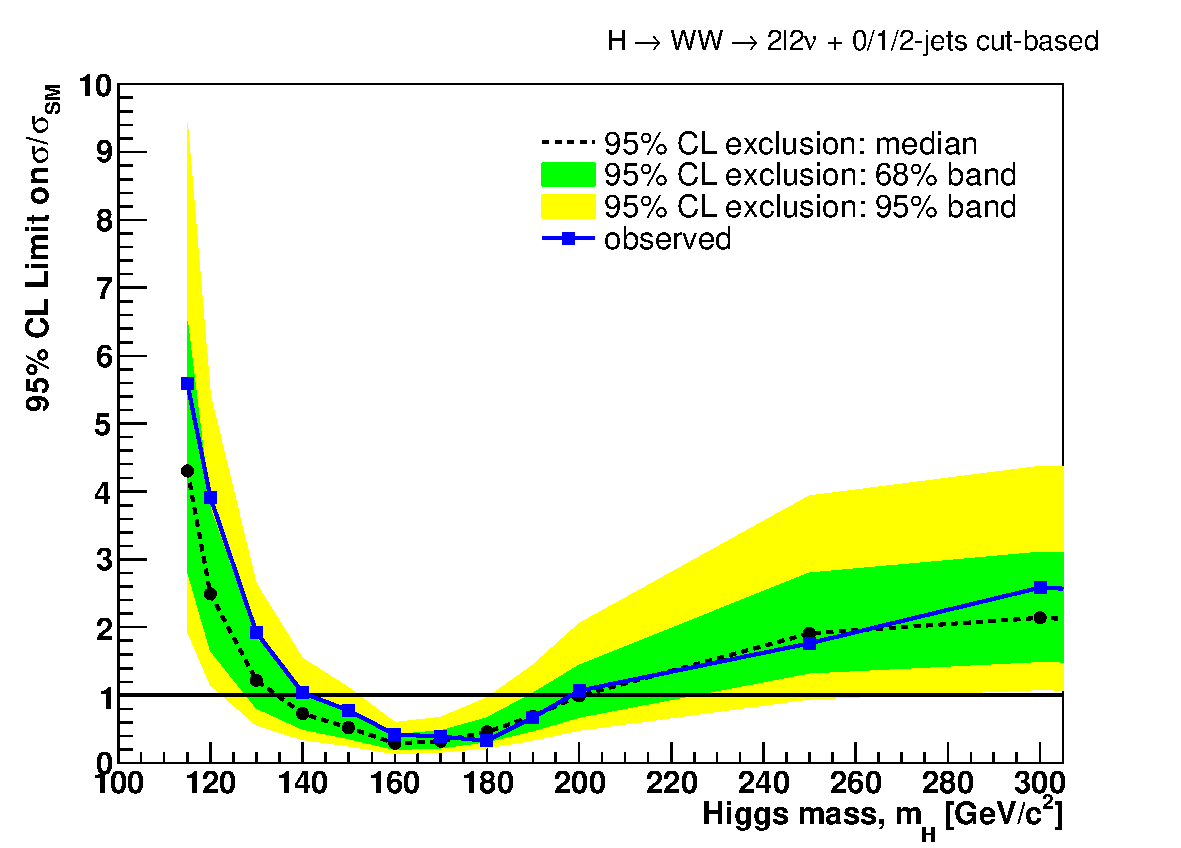
\includegraphics[width=0.48\textwidth]{lp_figures/limits_nj_cut_ana_v6_1500pb_LP.pdf}
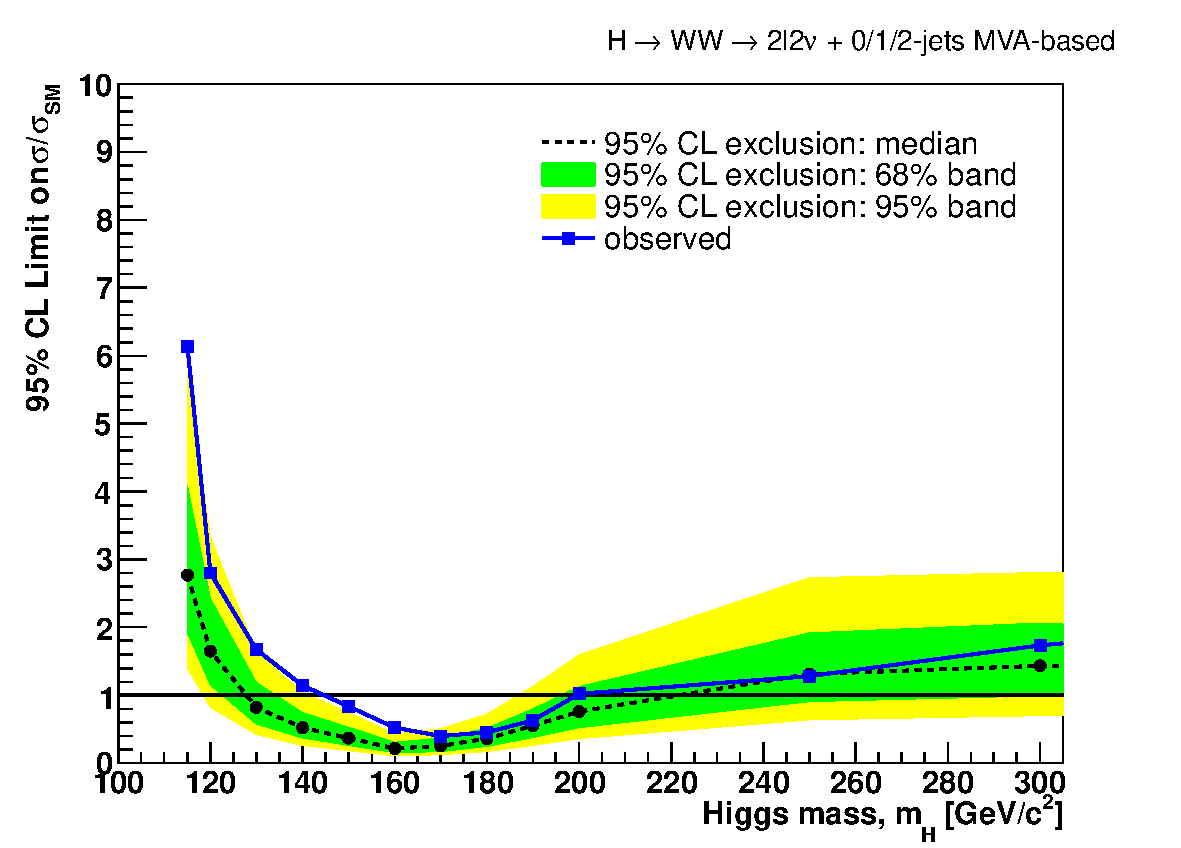
\includegraphics[width=0.48\textwidth]{lp_figures/limits_nj_shape_ana_v6_1500pb_LP.pdf}
\caption{Cut-based analysis (left) and multivariate-based analysis (right) upper limits at 95\% C.L. using data corresponding to 1.5~$\ifb$.
}
\label{fig:limits_final}
\end{figure}

In order to better understand the results we compared upper limit
results for EPS, post-EPS and full LP datasets in
Figures~\ref{fig:limits_0j_cut}-\ref{fig:limits_1j_shape}.

We notice that overall the post-EPS data show much better agreement
between observed and expected limits. In 0-jet case for same-flavor
events we see a downward fluctuation in both cut based and mva based
analyses (Figure~\ref{subfig:post_0j_sf_cut} and
\ref{subfig:post_0j_sf_shape}). In 1-jet case for same-flavor events
we see the observed limits to be consistent with the expected limits
(Figure~\ref{subfig:post_1j_sf_cut} and \ref{subfig:post_1j_sf_shape}
in both cut based and shape based analyses. It is different from the
EPS result (Figure~\ref{subfig:eps_1j_sf_cut} and
\ref{subfig:eps_1j_sf_shape}) that showed around 2$\sigma$ deviation
from the expected limits. This observation supports the idea that the
excess in 1-jet same-flavor events is likely to be just a fluctuation
and suggests that Drell-Yan background is under control.

\section{Additional Transverse Mass Selection Requirement}

We propose an additional selection requirement that can
be used to give extra confidence to the analysis. In general, a
requirement that $80 < M_T < m^{Higgs}$ would remove poorly understood
regions with only a negligible reduction in sensitivity.
Specifically, we refer to the following:

\begin{itemize}
    \item There is a concern that $W\gamma^*$ FSR background with
      $W\rightarrow \ell\nu$ and $\gamma^*\rightarrow\ell\ell$ could be
      a significant unaccounted background.  The $M_T$ of the
      reconstructed $e^{+}e^{-}$+MET system should be less than or
      equal to the expected $M_T$ from the decay of a $W$ boson.
    \item The \dytt~background is estimated entirely from simulation.
      This background manifests itself at low $M_T$, as illustrated in
      Figure~\ref{fig:ww_mthiggs_lp}.
    \item Other backgrounds such as W+jets and WW are reduced by
      removing the low $M_T$ region.
\end{itemize}

The yield cross check using same-sign events bounds the $W/\gamma*$ background 
at something less than 10 events at WW preselection level.  
This bound has the caveat that if the background is large and the 
fake rate method understimates the real background then the two
effects can cancel.

The default conversion rejection algorithm used in this analysis
includes a 2 cm flight distance (Lxy) cut, so would not reject this background
from apparently prompt conversions.
Taking into account the expected efficiency of our conversion
rejection algorithm, and removing the Lxy cut, 
we would expect to reject $30-50$\% of the residual 
$\gamma*\rightarrow e^{+}e^{-}$ background.
Performing this test we remove four events at the WW preselection level.
This reduction in the observed yield is consistent with expectations
from WW, W+jet and W+$\gamma$ simulation.
The events removed are distributed randomly in $M_T$.

Although we do not find evidence of a large unaccounted $W/\gamma*$ background,
we cannot conclusively prove that it is absent either.
We note that the proposed cut would reduce the \dytt~background from an expectation
of around 13 events to below one event in the one-jet bin $e-\mu$ final state at
the MVA preselection level.

\begin{figure}[!htbp]
\centering
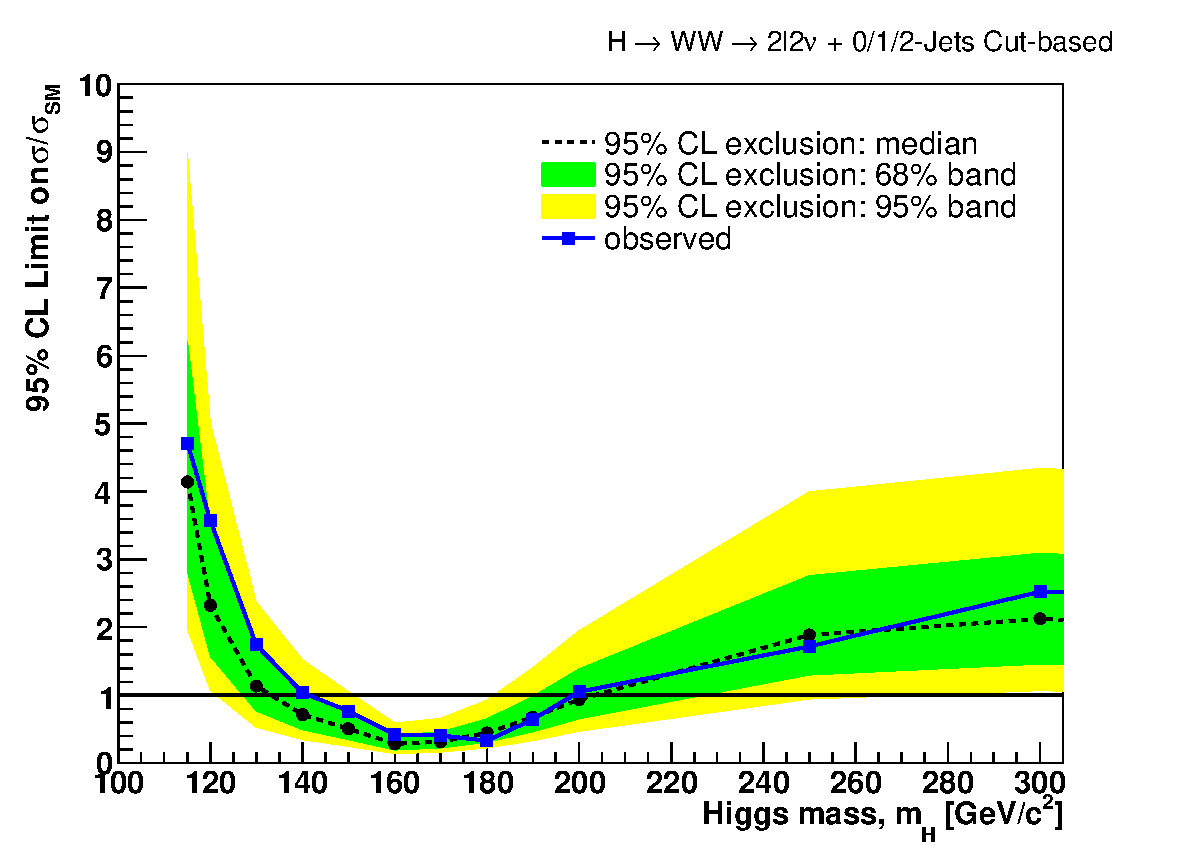
\includegraphics[width=0.48\textwidth]{lp_figures/limits_nj_cut_ana_v6_1500pb_LP_MTCUT80.pdf}
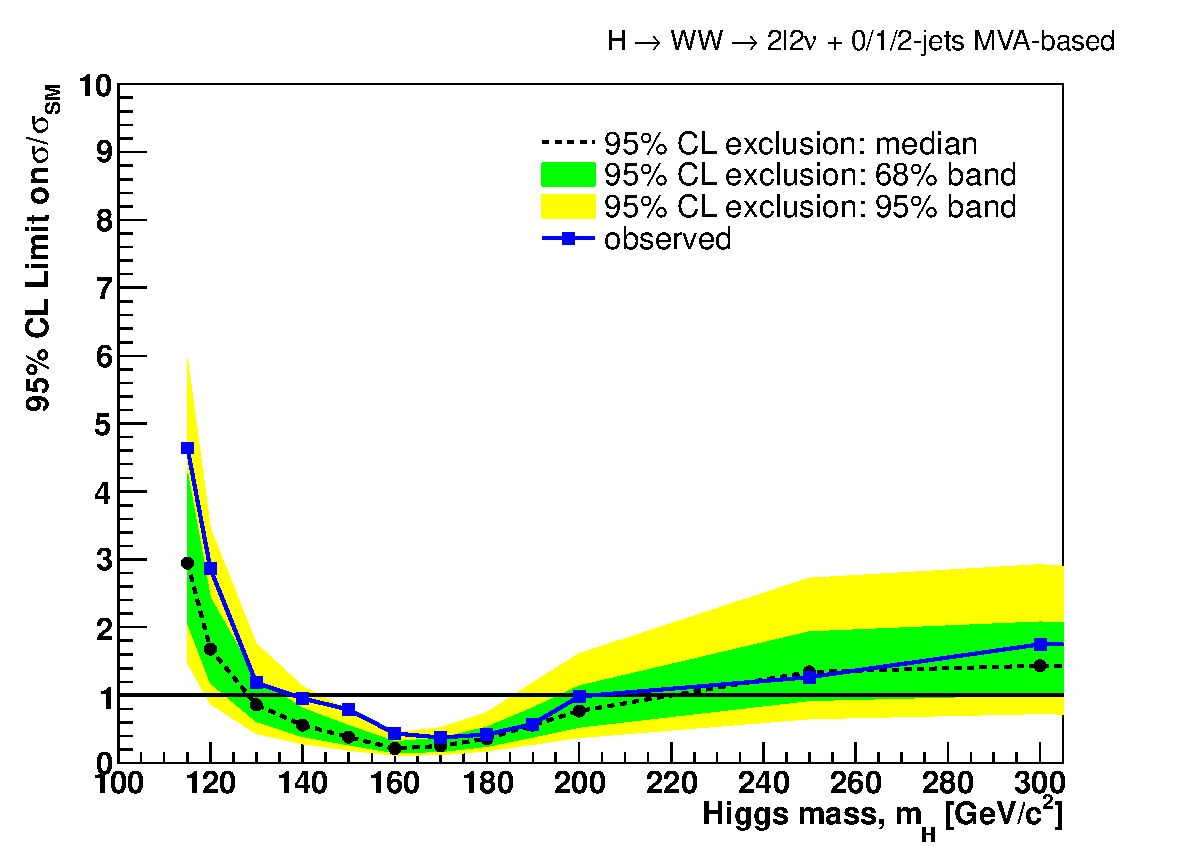
\includegraphics[width=0.48\textwidth]{lp_figures/limits_nj_shape_ana_v6_1500pb_LP_MTCUT80.pdf}
\caption{Cut-based analysis (left) and multivariate-based analysis (right) upper limits at 95\% C.L. 
using data corresponding to 1.5~$\ifb$ applying the additional $m_T$ cut.}
\label{fig:limits_final_mt80}
\end{figure}

Figures \ref{fig:limits_final_mt80}, \ref{fig:limits_lp_mtcut80_cut} and
\ref{fig:limits_lp_mtcut80_shape} show results with the $M_T$ cut
applied. It has negligible effect on the expected analysis sensitivity
at all mass points. The observed limits get closer to the expected
ones at low Higgs mass points. This can be either a background
reduction effected or a statistical fluctuation.

\section{Conclusions}

The H$\to$WW$\to2l2\nu$ analysis was successfully updated for the
Lepton Photon 2011 conference. The results obtained in the post-EPS
dataset were found to be consistent with the results from the EPS
analysis, thus the two were combined to perform the update.

The EPS counting analysis indicated an excess in the same flavor final
state, both in the 0-jet Higgs boson mass range ~150-170GeV region and
the 1-jet analysis over the full mass range.  This trend is not
evident in the post-EPS dataset.

We conclude that adding the post-EPS dataset to this analysis 
supports the hypothesis that same flavor excesses in the EPS
analysis are more likely attributed to statistical fluctuation
than a systematic bias in Drell-Yan estimation.

Evidence has been presented that the robustness of the analysis can be
improved by the addition of a cut to remove events with an $M_T$
inconsistent with the signal hypothesis. We advocate to use this
selection requirement to reduce contribution of poorly understood
backgrounds to the analysis.

The Higgs exclusion limits are [140-200] GeV for the cut-based analysis and
[144-200] for the multivariate analysis. 

%%%%%%%%%%%%%%%%%%%%%%%%%%%%%%
\begin{figure}[!htbp]
\centering
\subfigure[]{
\centering
\label{subfig:lp_0j_sf_cut}
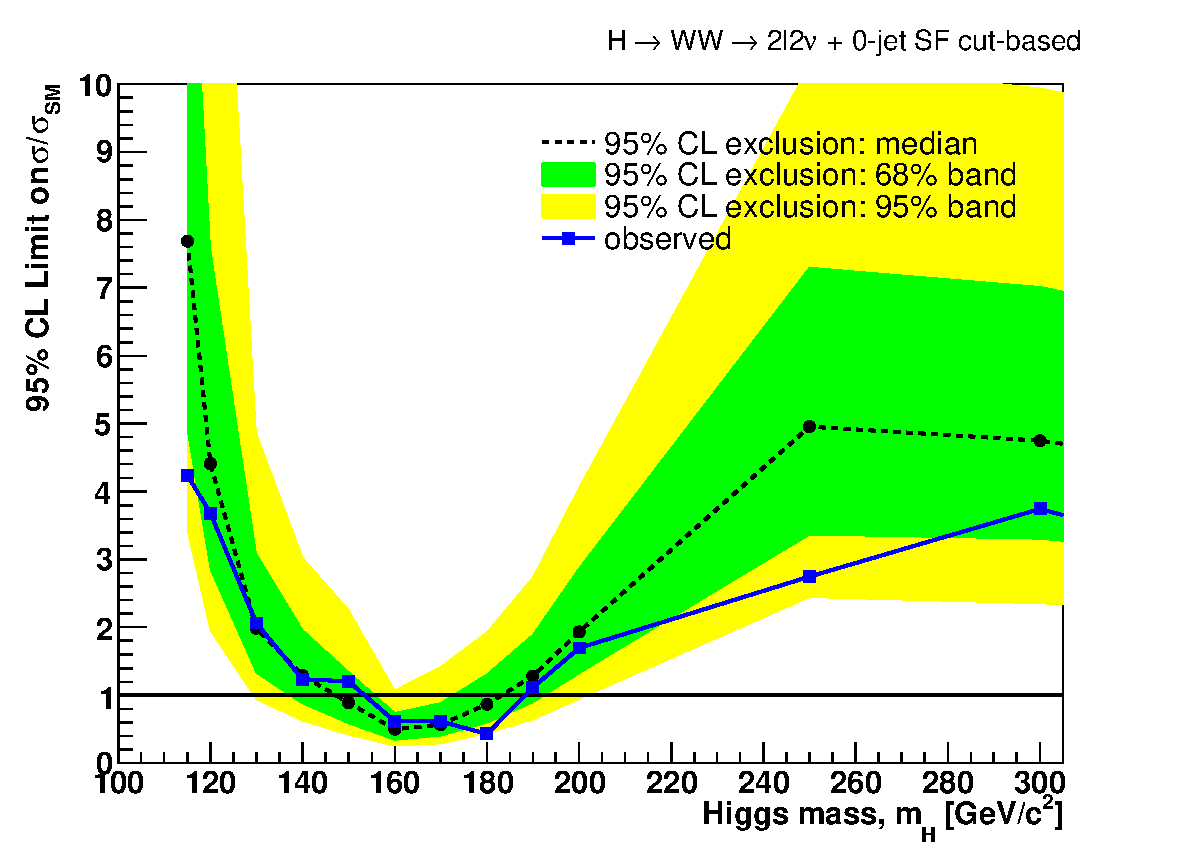
\includegraphics[width=0.48\textwidth]{lp_figures/limits_0j_sf_cut.pdf}}
\subfigure[]{
\centering
\label{subfig:lp_0j_of_cut}
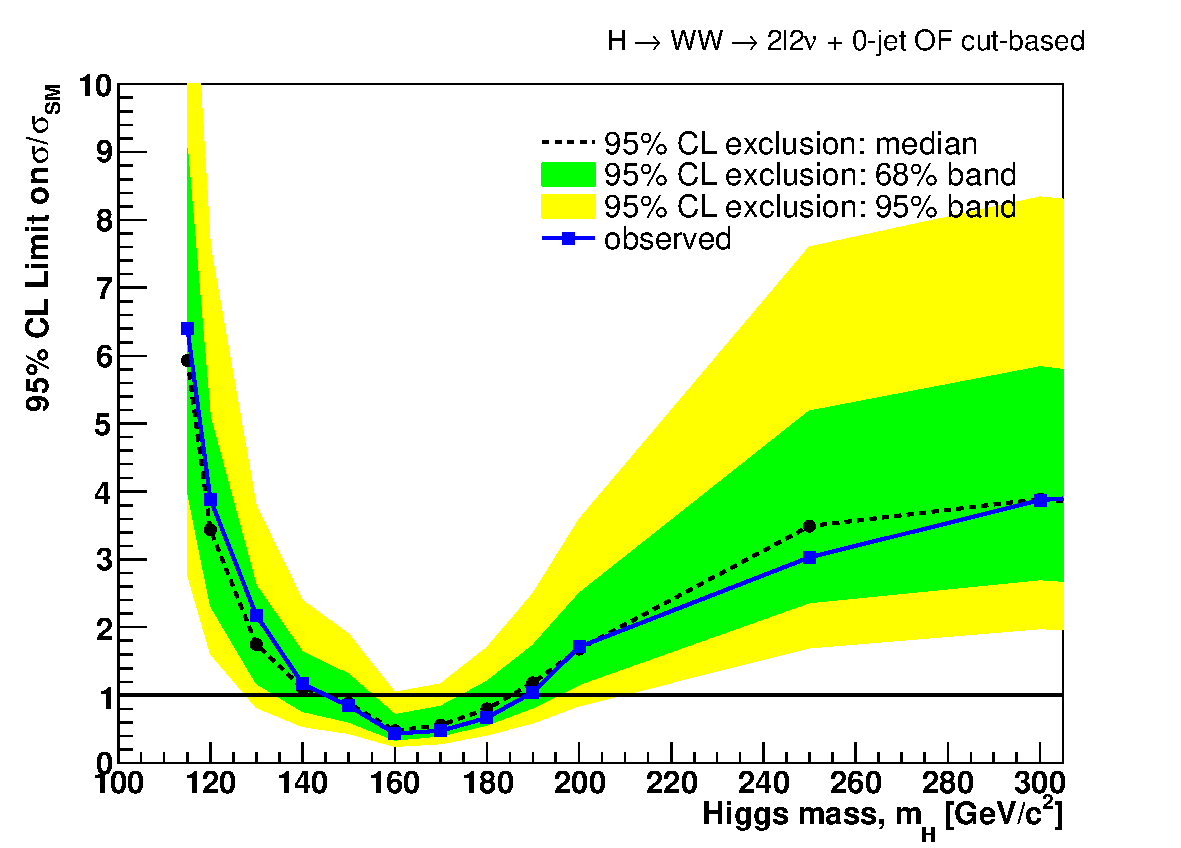
\includegraphics[width=0.48\textwidth]{lp_figures/limits_0j_of_cut.pdf}}
\subfigure[]{
\centering
\label{subfig:eps_0j_sf_cut}
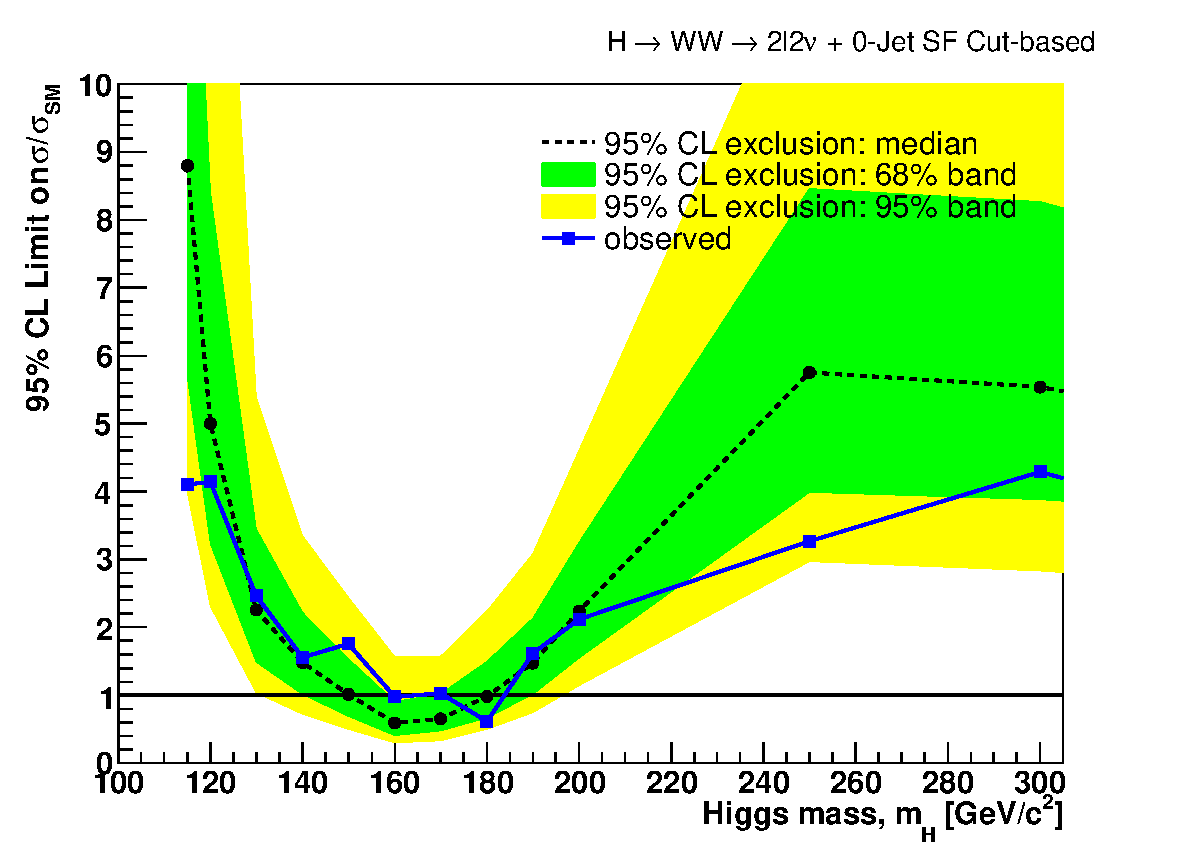
\includegraphics[width=0.48\textwidth]{lp_figures/limits_0j_sf_cut_ana_v6_1500pb_LP_EPS.pdf}}
\subfigure[]{
\centering
\label{subfig:eps_0j_of_cut}
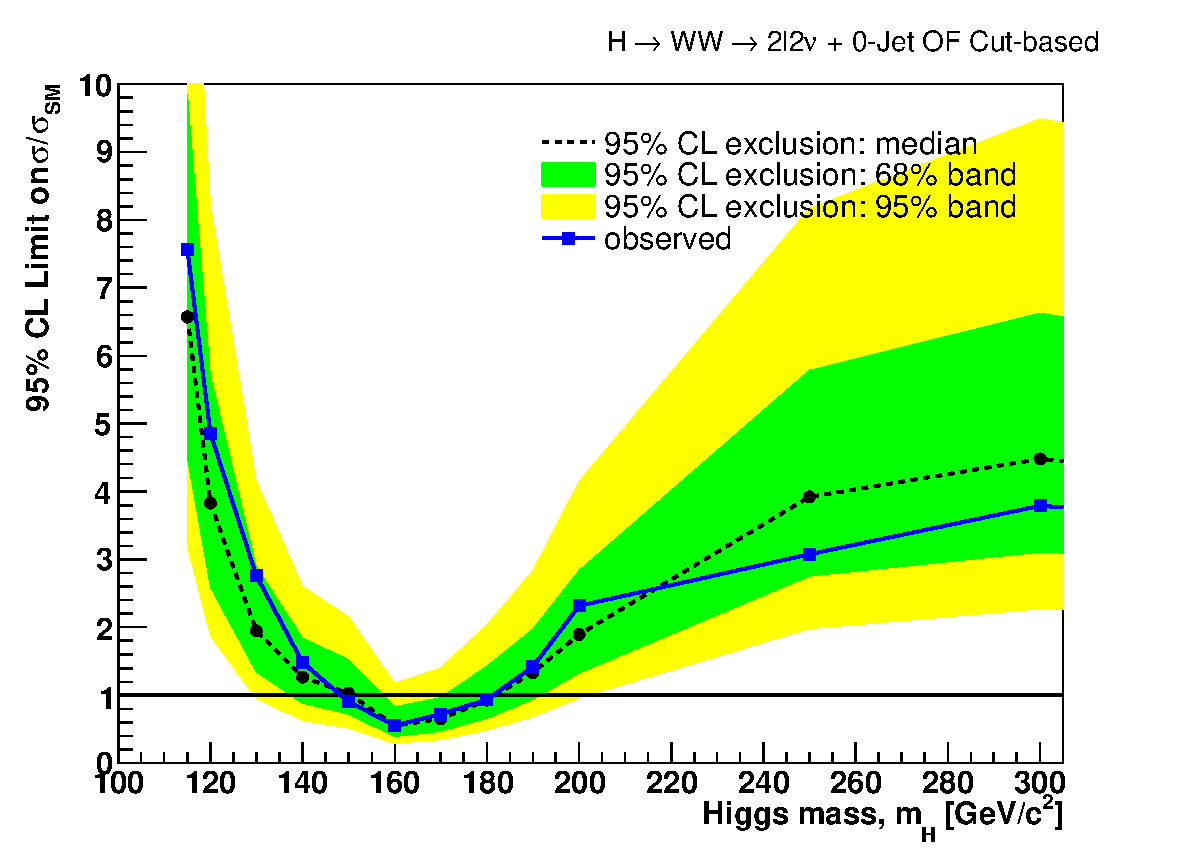
\includegraphics[width=0.48\textwidth]{lp_figures/limits_0j_of_cut_ana_v6_1500pb_LP_EPS.pdf}}
\subfigure[]{
\centering
\label{subfig:post_0j_sf_cut}
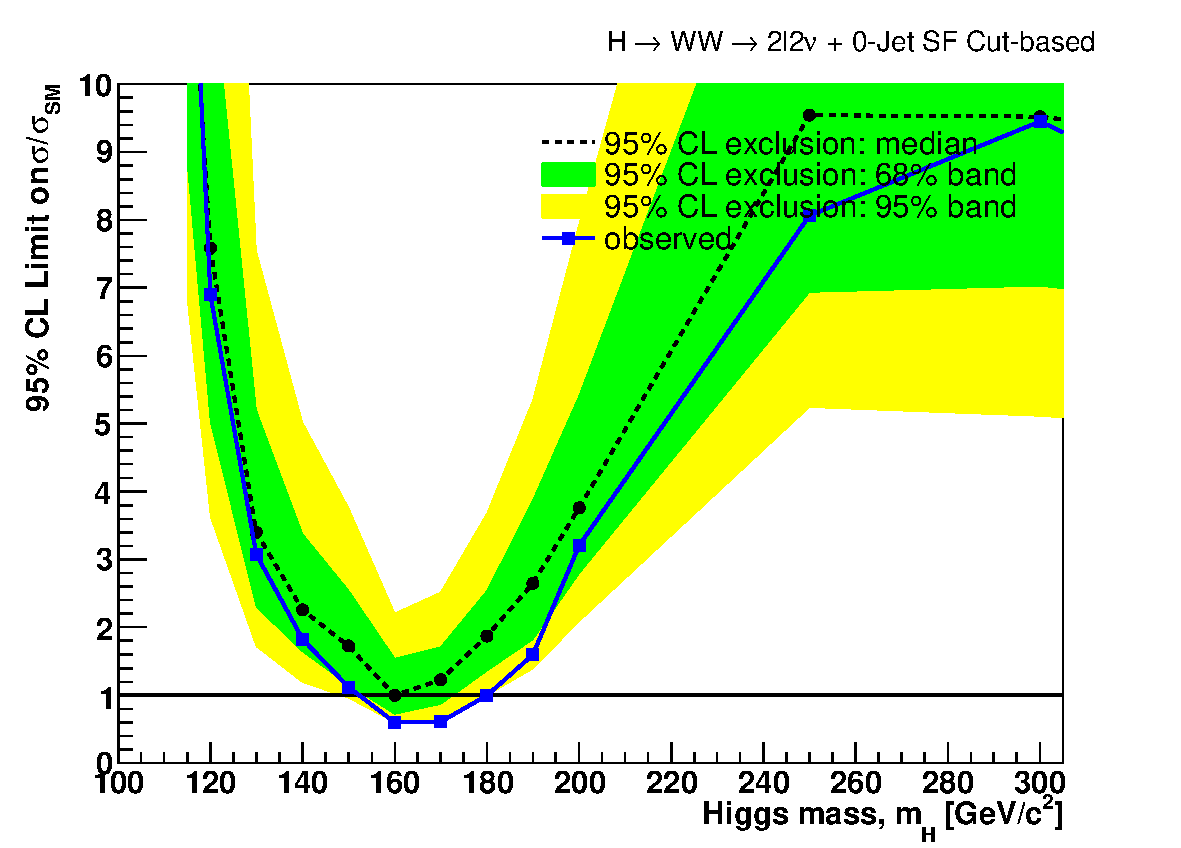
\includegraphics[width=0.48\textwidth]{lp_figures/limits_0j_sf_cut_ana_v6_1500pb_LP_POSTEPS.pdf}}
\subfigure[]{
\centering
\label{subfig:post_0j_of_cut}
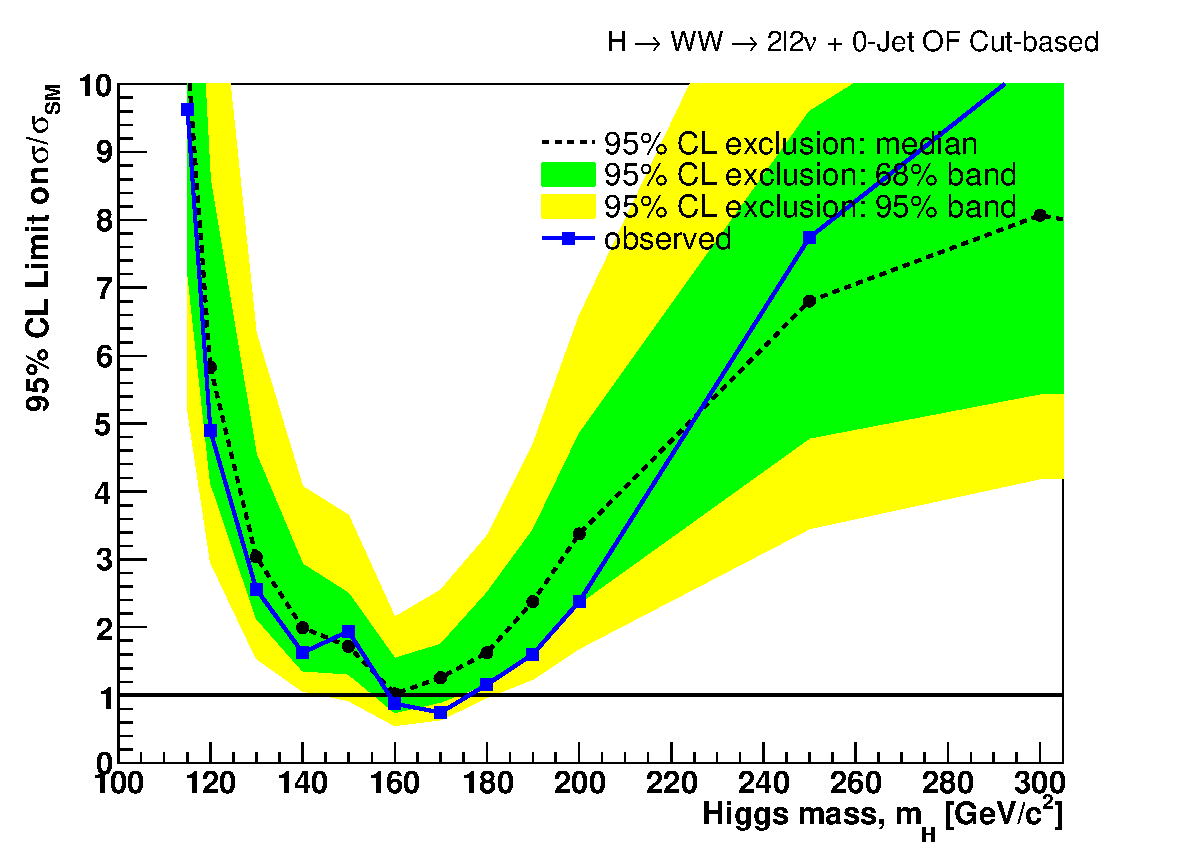
\includegraphics[width=0.48\textwidth]{lp_figures/limits_0j_of_cut_ana_v6_1500pb_LP_POSTEPS.pdf}}
\caption{Cut-based analysis upper limits at 95\% C.L. using LP, EPS and post-EPS datasets for 0-jet events.
\subref{subfig:lp_0j_sf_cut}: LP same-flavor; \subref{subfig:lp_0j_of_cut}: LP opposite-flavor; 
\subref{subfig:eps_0j_sf_cut}: EPS same-flavor; \subref{subfig:eps_0j_of_cut}: EPS opposite-flavor; 
\subref{subfig:post_0j_sf_cut}: post-EPS same-flavor; \subref{subfig:post_0j_of_cut}: post-EPS opposite-flavor; 
}
\label{fig:limits_0j_cut}
\end{figure}


\begin{figure}[!htbp]
\centering
\subfigure[]{
\centering
\label{subfig:lp_0j_sf_shape}
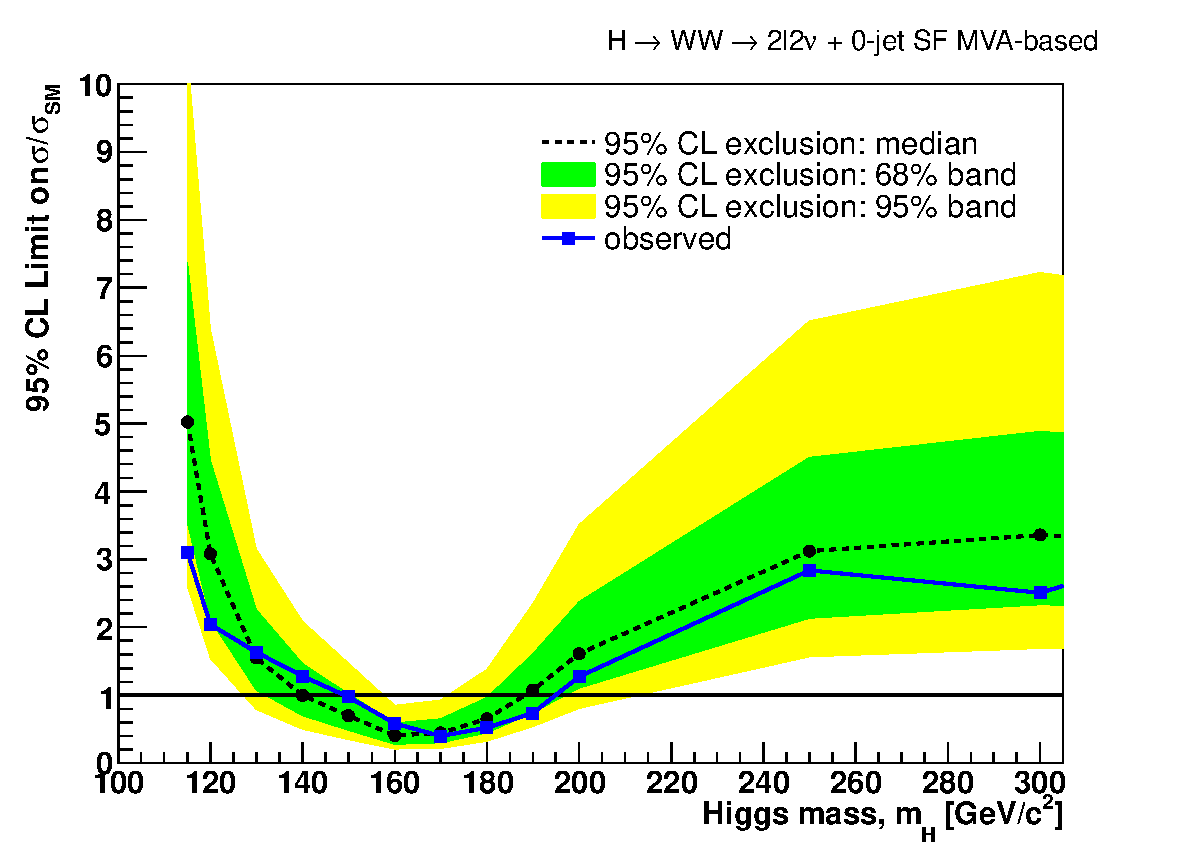
\includegraphics[width=0.48\textwidth]{lp_figures/limits_0j_sf_shape.pdf}}
\subfigure[]{
\centering
\label{subfig:lp_0j_of_shape}
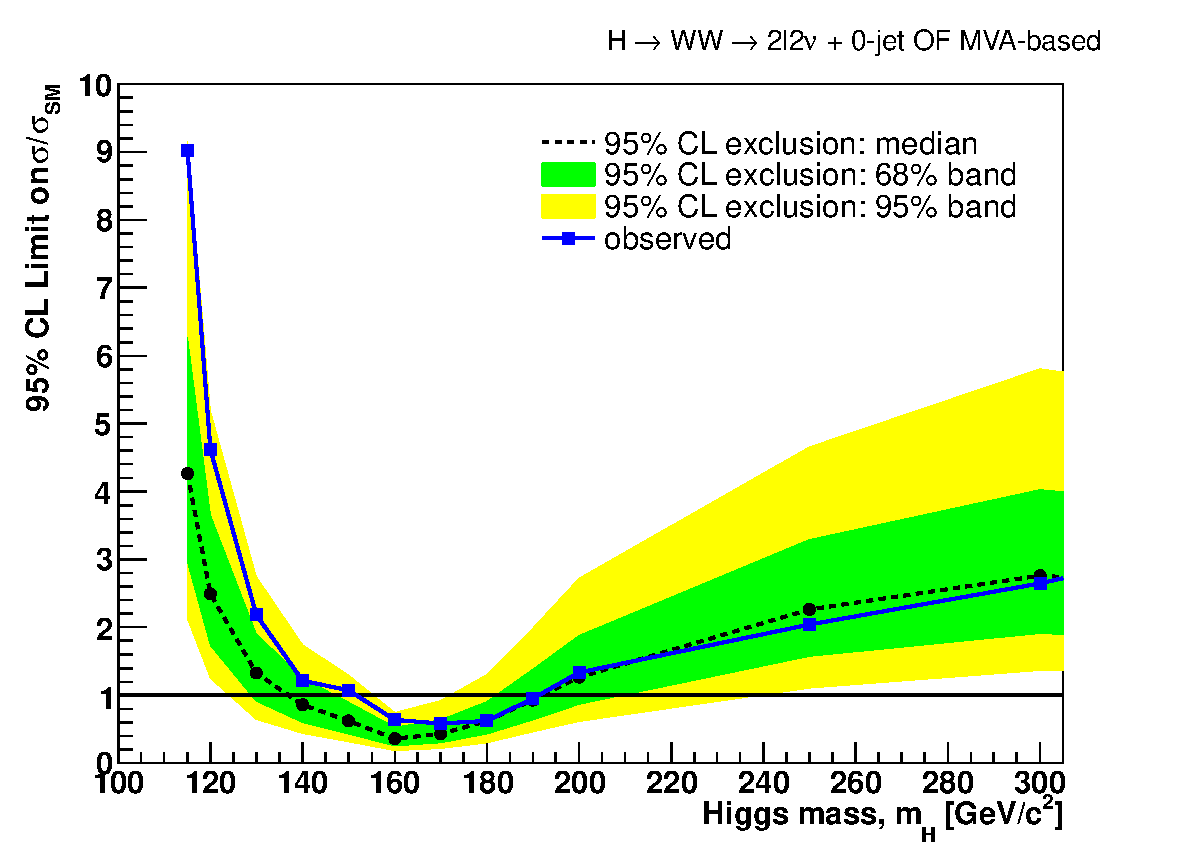
\includegraphics[width=0.48\textwidth]{lp_figures/limits_0j_of_shape.pdf}}
\subfigure[]{
\centering
\label{subfig:eps_0j_sf_shape}
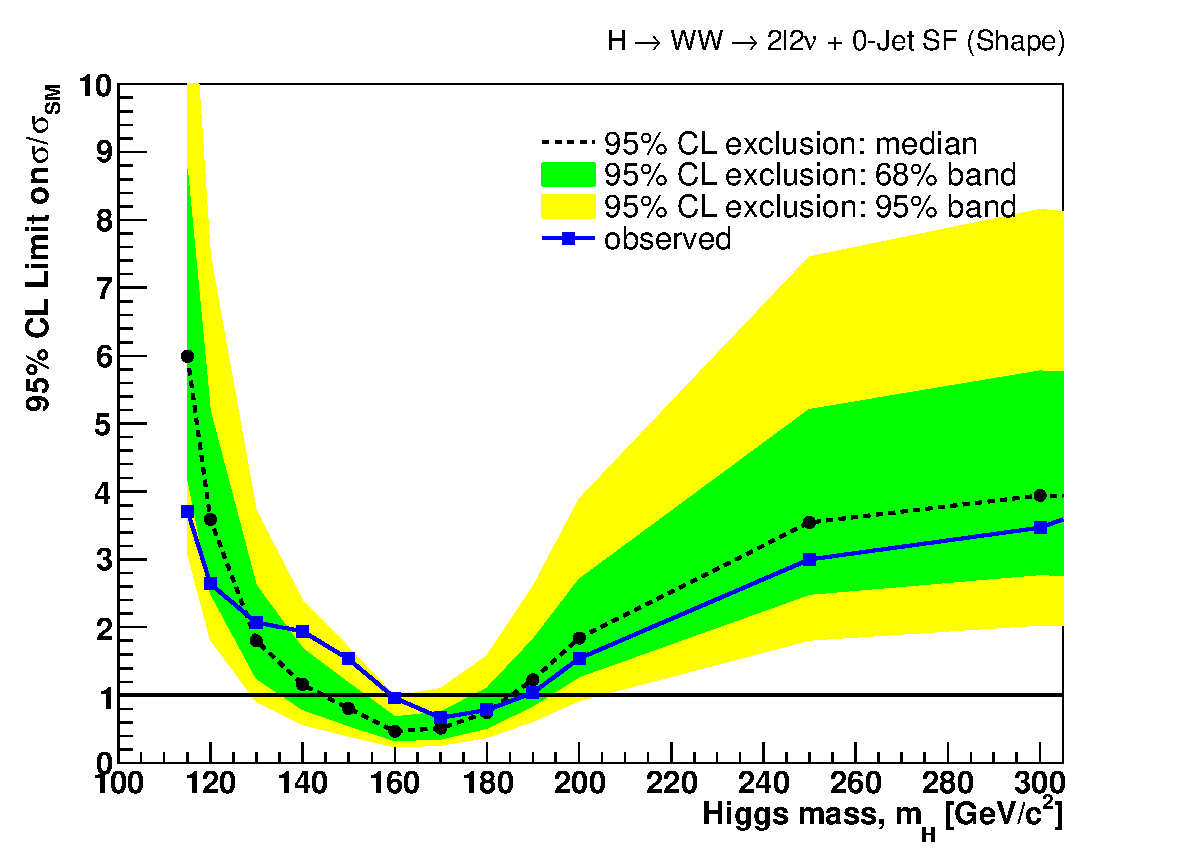
\includegraphics[width=0.48\textwidth]{lp_figures/limits_0j_sf_shape_ana_v6_1500pb_LP_EPS.pdf}}
\subfigure[]{
\centering
\label{subfig:eps_0j_of_shape}
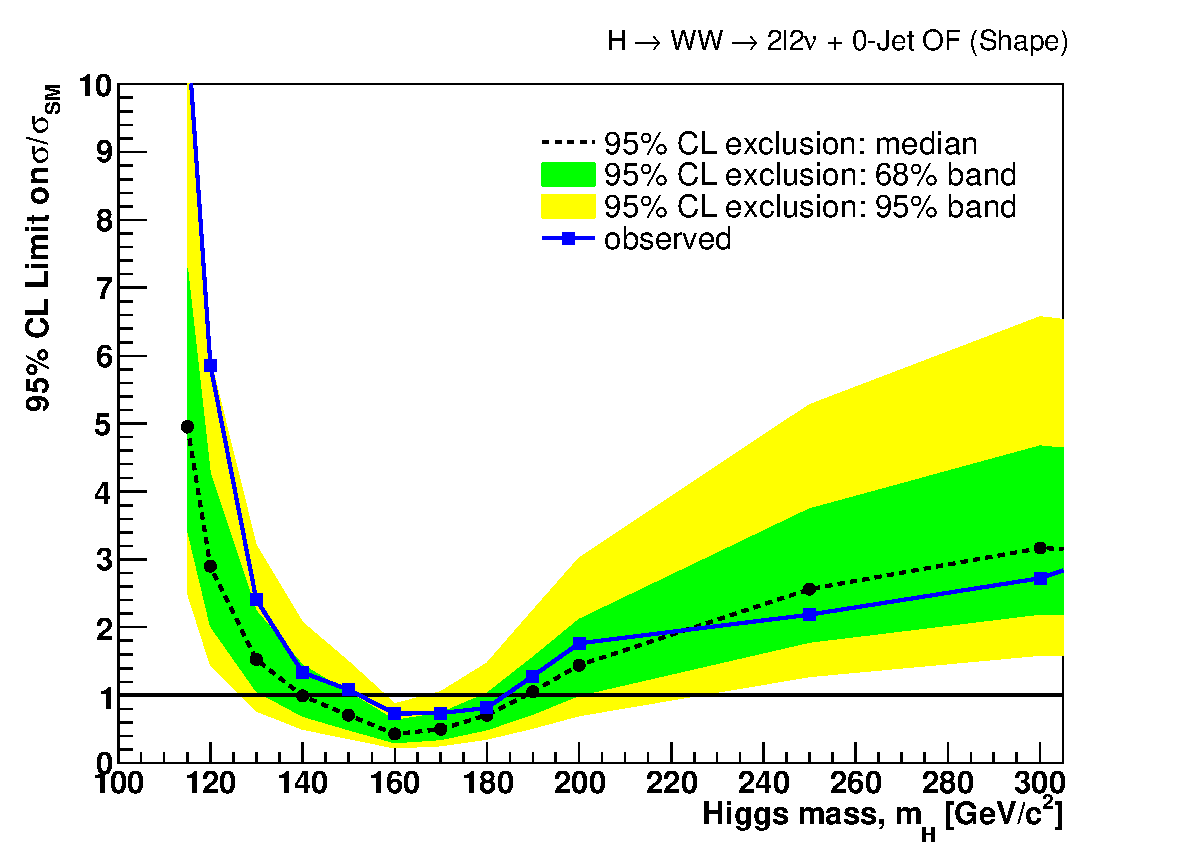
\includegraphics[width=0.48\textwidth]{lp_figures/limits_0j_of_shape_ana_v6_1500pb_LP_EPS.pdf}}
\subfigure[]{
\centering
\label{subfig:post_0j_sf_shape}
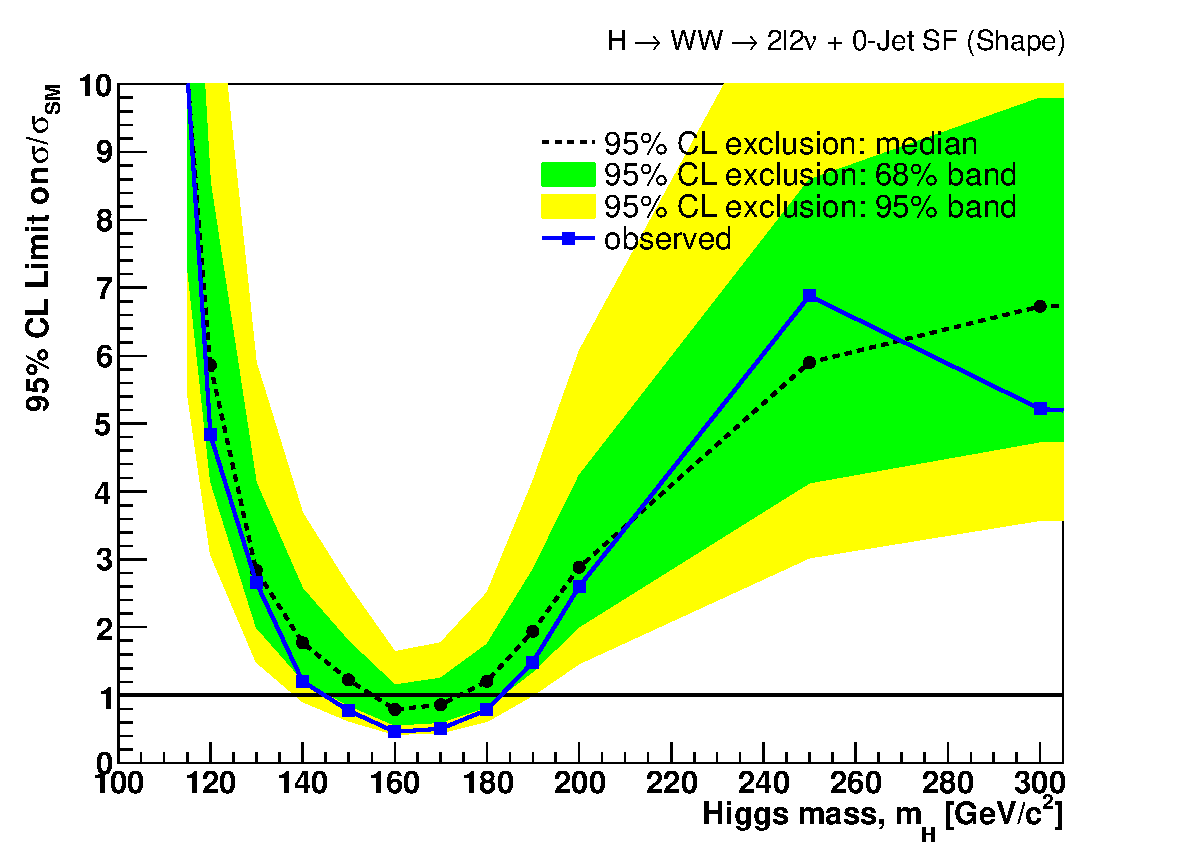
\includegraphics[width=0.48\textwidth]{lp_figures/limits_0j_sf_shape_ana_v6_1500pb_LP_POSTEPS.pdf}}
\subfigure[]{
\centering
\label{subfig:post_0j_of_shape}
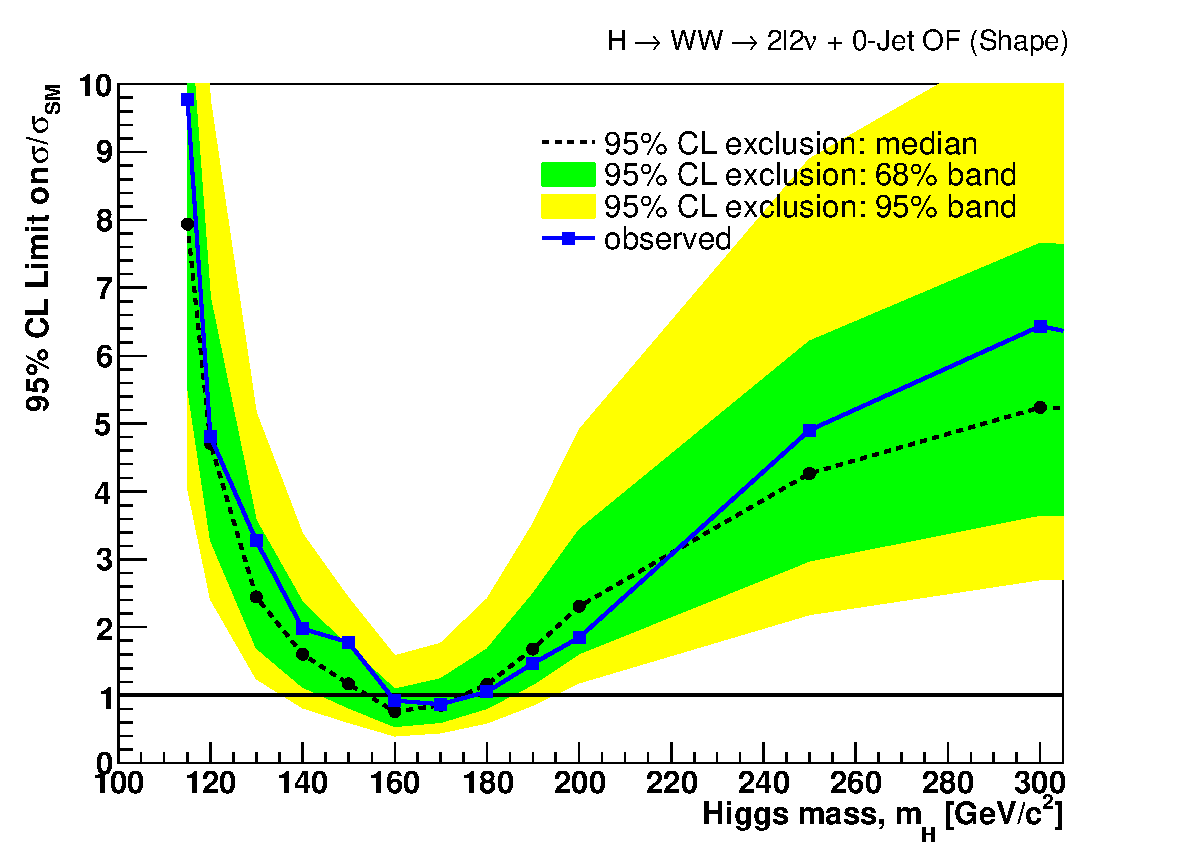
\includegraphics[width=0.48\textwidth]{lp_figures/limits_0j_of_shape_ana_v6_1500pb_LP_POSTEPS.pdf}}
\caption{Multivariate-based analysis upper limits at 95\% C.L. using LP, EPS and post-EPS datasets for 0-jet events.
\subref{subfig:lp_0j_sf_shape}: LP same-flavor; \subref{subfig:lp_0j_of_shape}: LP opposite-flavor; 
\subref{subfig:eps_0j_sf_shape}: EPS same-flavor; \subref{subfig:eps_0j_of_shape}: EPS opposite-flavor; 
\subref{subfig:post_0j_sf_shape}: post-EPS same-flavor; \subref{subfig:post_0j_of_shape}: post-EPS opposite-flavor; 
}
\label{fig:limits_0j_shape}
\end{figure}

\begin{figure}[!htbp]
\centering
\subfigure[]{
\centering
\label{subfig:lp_1j_sf_cut}
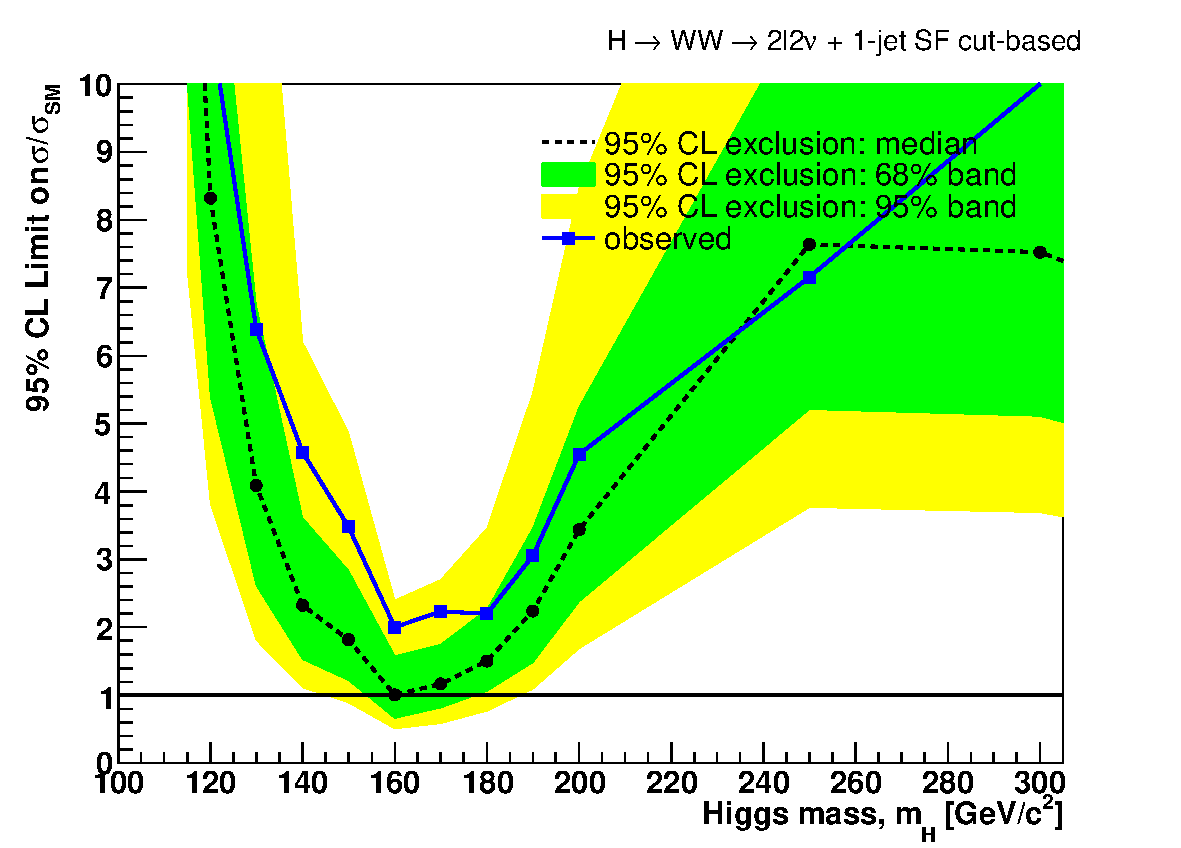
\includegraphics[width=0.48\textwidth]{lp_figures/limits_1j_sf_cut.pdf}}
\subfigure[]{
\centering
\label{subfig:lp_1j_of_cut}
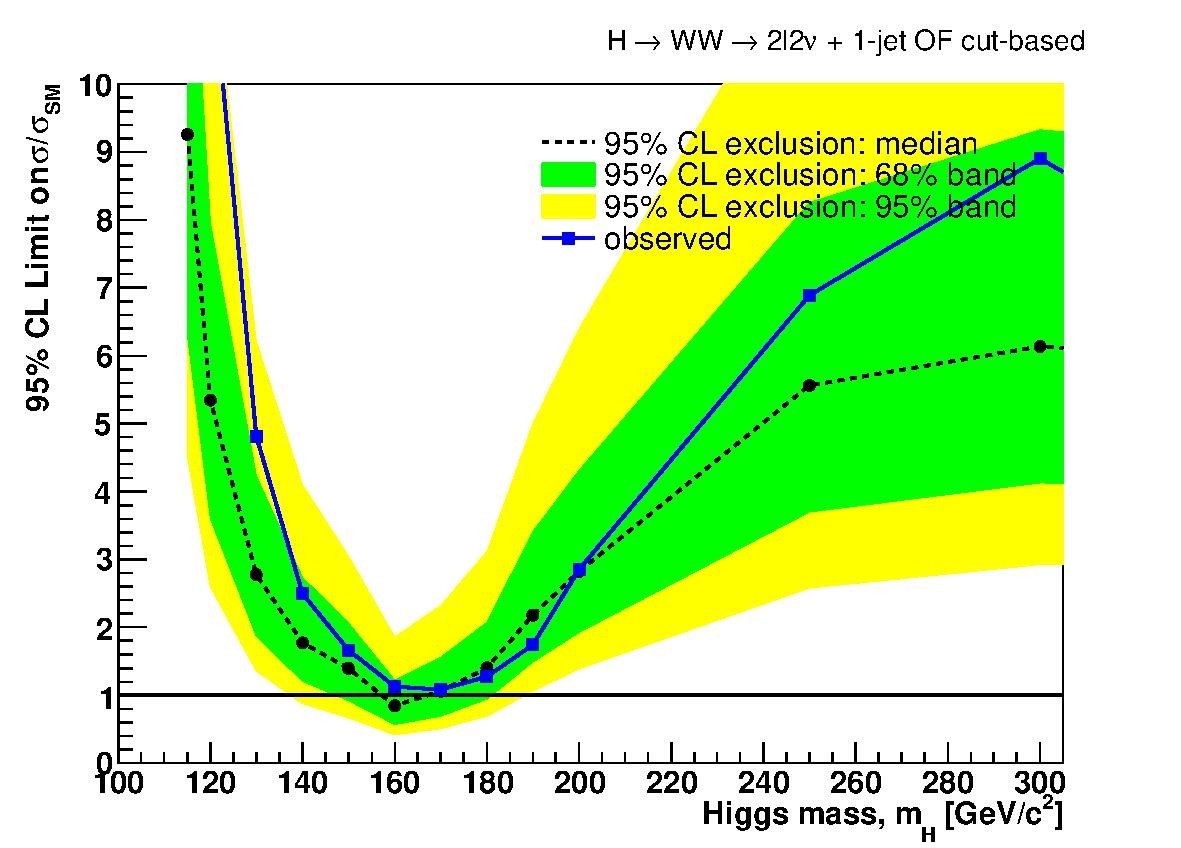
\includegraphics[width=0.48\textwidth]{lp_figures/limits_1j_of_cut.pdf}}
\subfigure[]{
\centering
\label{subfig:eps_1j_sf_cut}
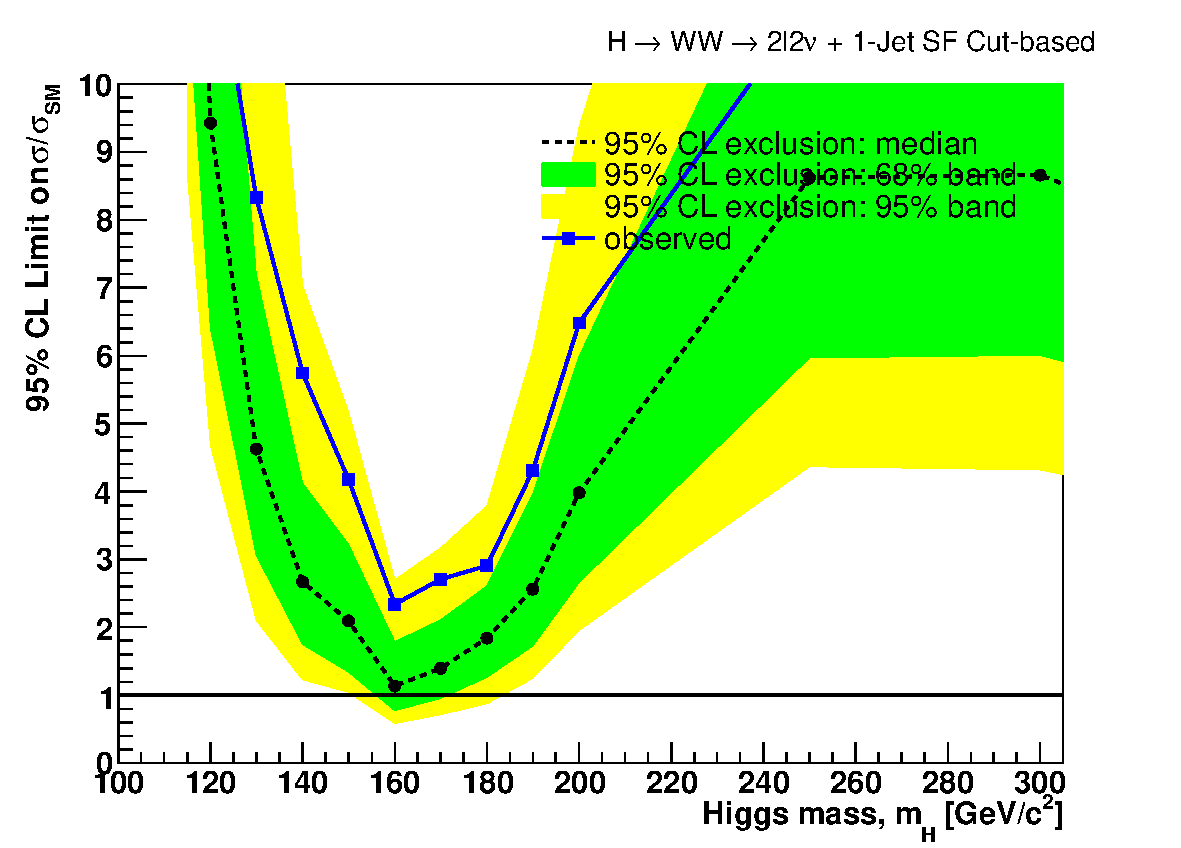
\includegraphics[width=0.48\textwidth]{lp_figures/limits_1j_sf_cut_ana_v6_1500pb_LP_EPS.pdf}}
\subfigure[]{
\centering
\label{subfig:eps_1j_of_cut}
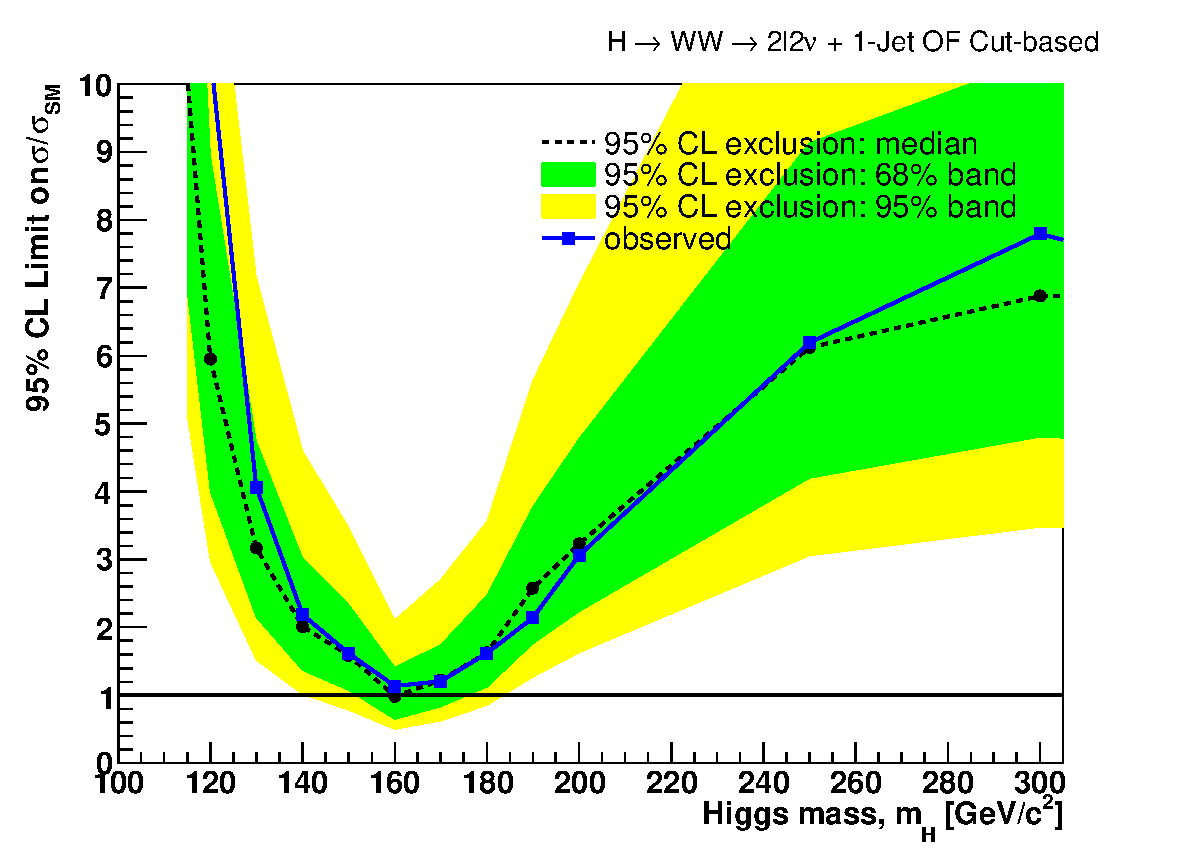
\includegraphics[width=0.48\textwidth]{lp_figures/limits_1j_of_cut_ana_v6_1500pb_LP_EPS.pdf}}
\subfigure[]{
\centering
\label{subfig:post_1j_sf_cut}
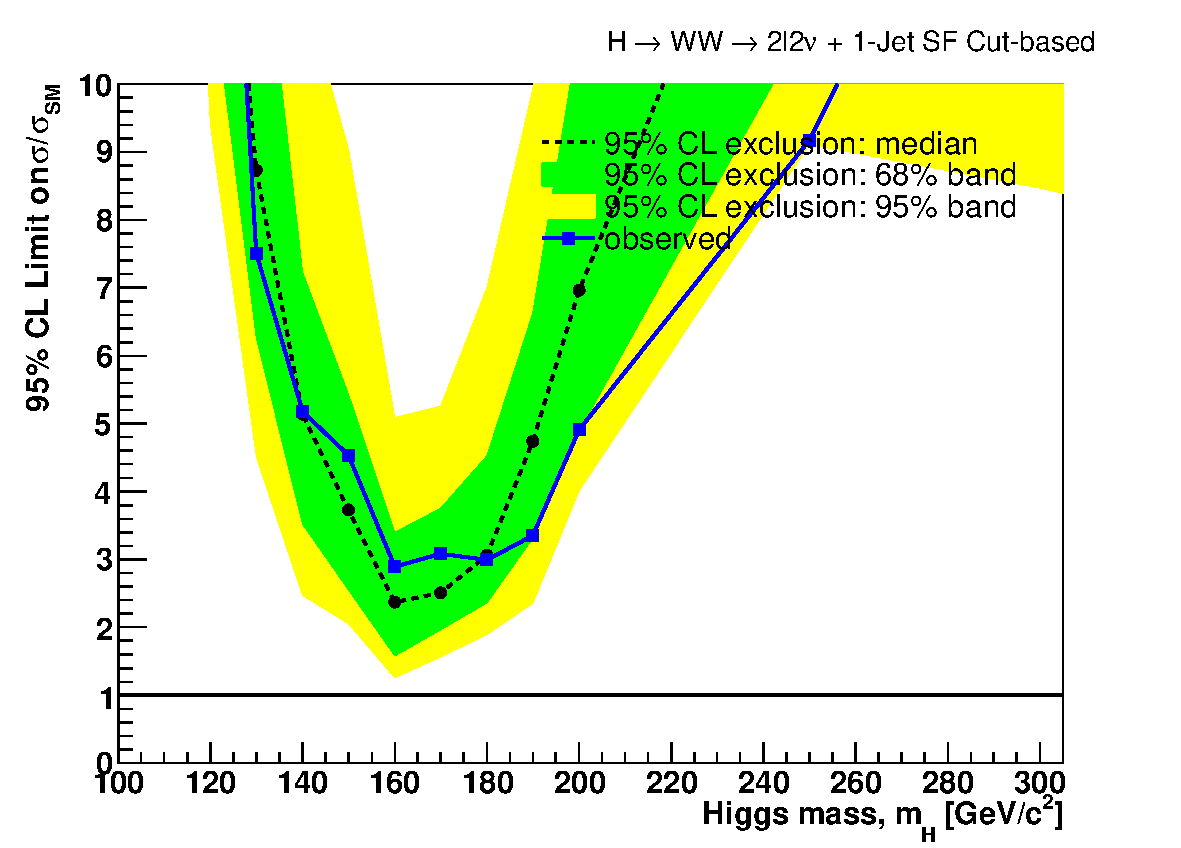
\includegraphics[width=0.48\textwidth]{lp_figures/limits_1j_sf_cut_ana_v6_1500pb_LP_POSTEPS.pdf}}
\subfigure[]{
\centering
\label{subfig:post_1j_of_cut}
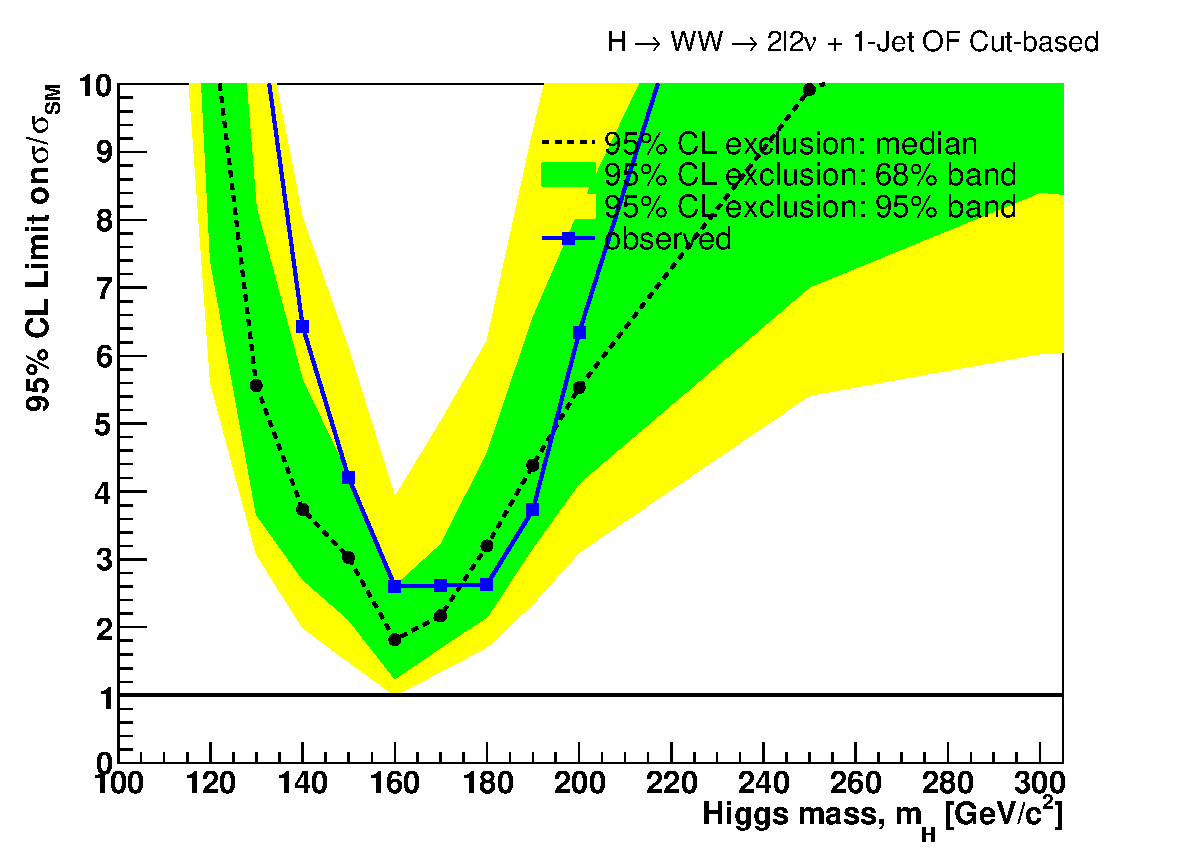
\includegraphics[width=0.48\textwidth]{lp_figures/limits_1j_of_cut_ana_v6_1500pb_LP_POSTEPS.pdf}}
\caption{Cut-based analysis upper limits at 95\% C.L. using LP, EPS and post-EPS datasets for 1-jet events.
\subref{subfig:lp_1j_sf_cut}: LP same-flavor; \subref{subfig:lp_1j_of_cut}: LP opposite-flavor; 
\subref{subfig:eps_1j_sf_cut}: EPS same-flavor; \subref{subfig:eps_1j_of_cut}: EPS opposite-flavor; 
\subref{subfig:post_1j_sf_cut}: post-EPS same-flavor; \subref{subfig:post_1j_of_cut}: post-EPS opposite-flavor; 
}
\label{fig:limits_1j_cut}
\end{figure}

\begin{figure}[!htbp]
\centering
\subfigure[]{
\centering
\label{subfig:lp_1j_sf_shape}
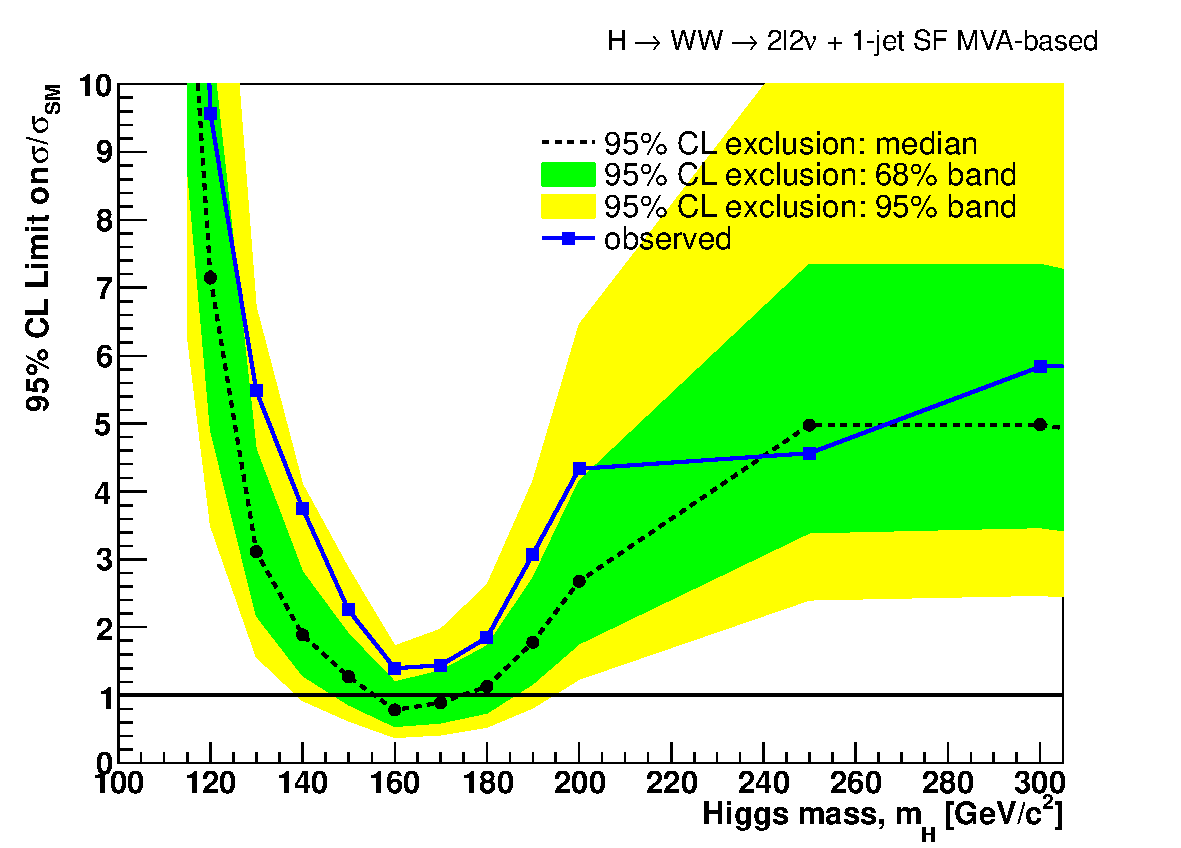
\includegraphics[width=0.48\textwidth]{lp_figures/limits_1j_sf_shape.pdf}}
\subfigure[]{
\centering
\label{subfig:lp_1j_of_shape}
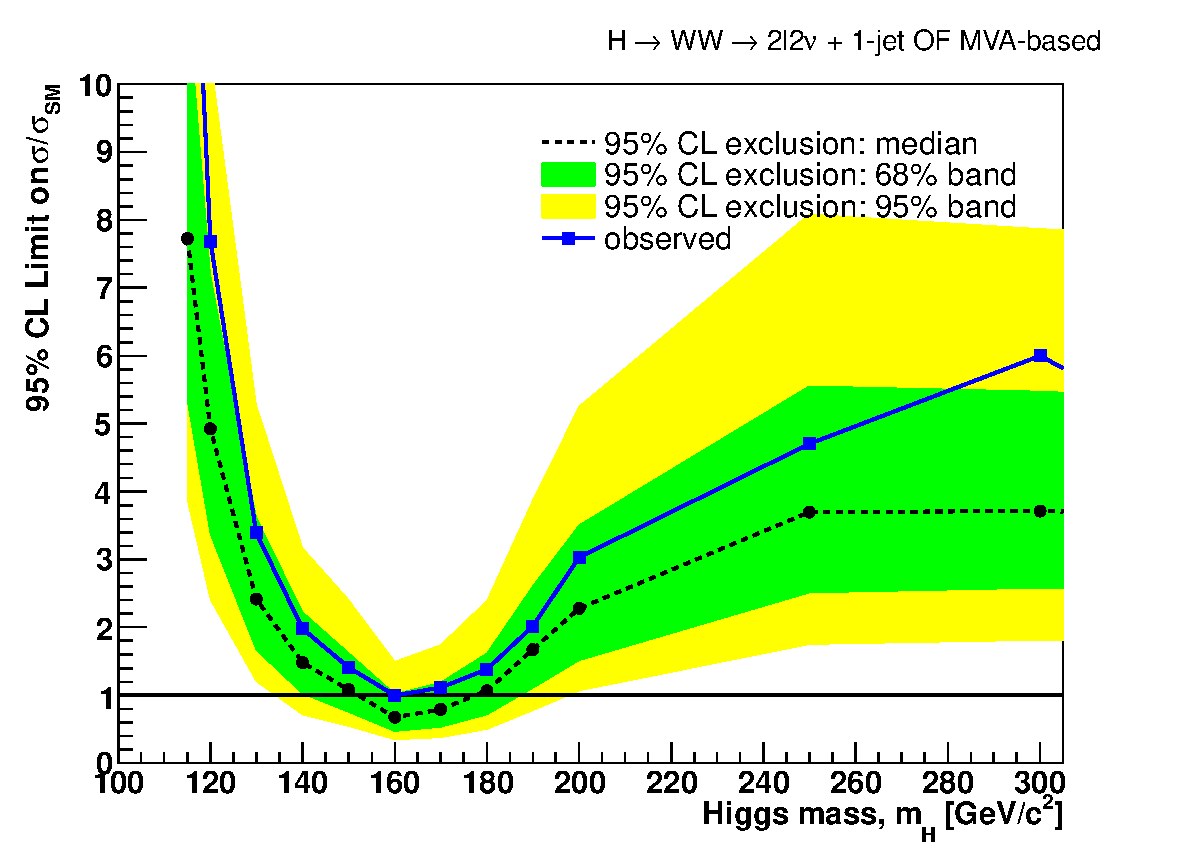
\includegraphics[width=0.48\textwidth]{lp_figures/limits_1j_of_shape.pdf}}
\subfigure[]{
\centering
\label{subfig:eps_1j_sf_shape}
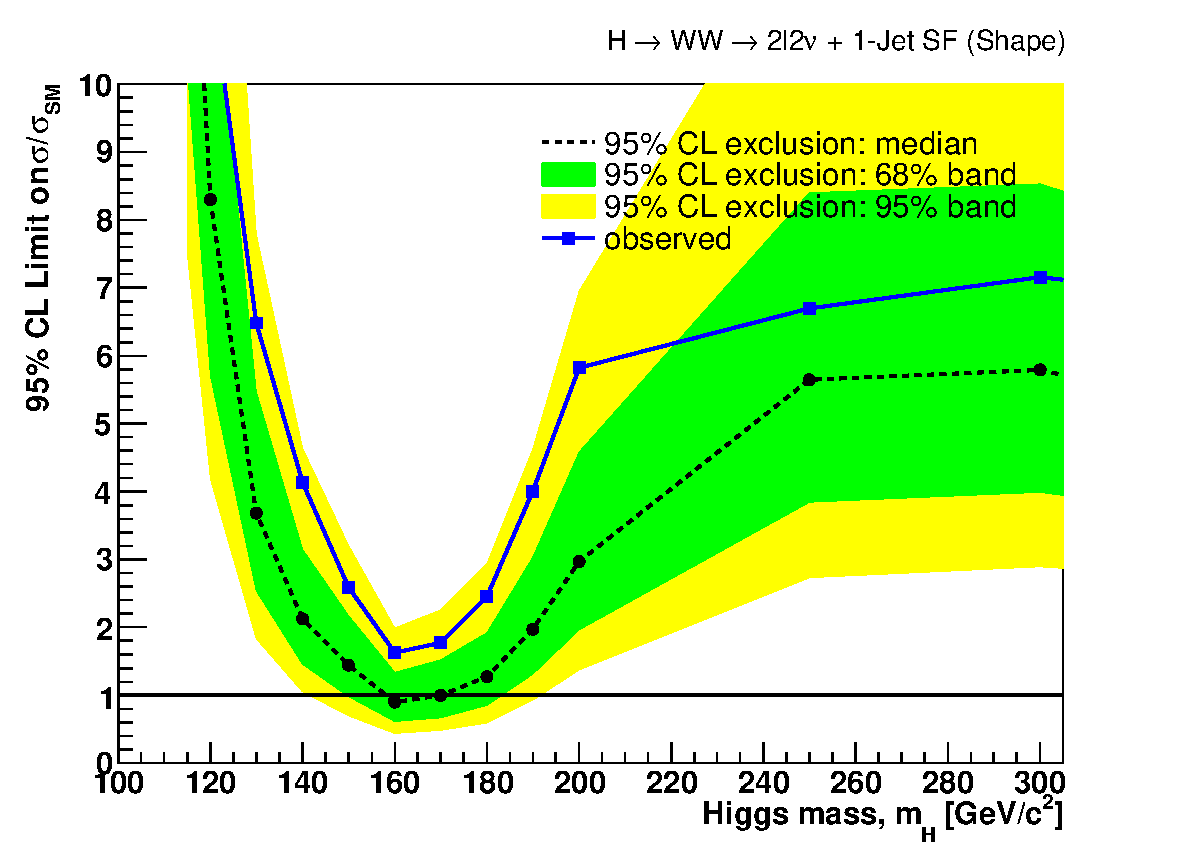
\includegraphics[width=0.48\textwidth]{lp_figures/limits_1j_sf_shape_ana_v6_1500pb_LP_EPS.pdf}}
\subfigure[]{
\centering
\label{subfig:eps_1j_of_shape}
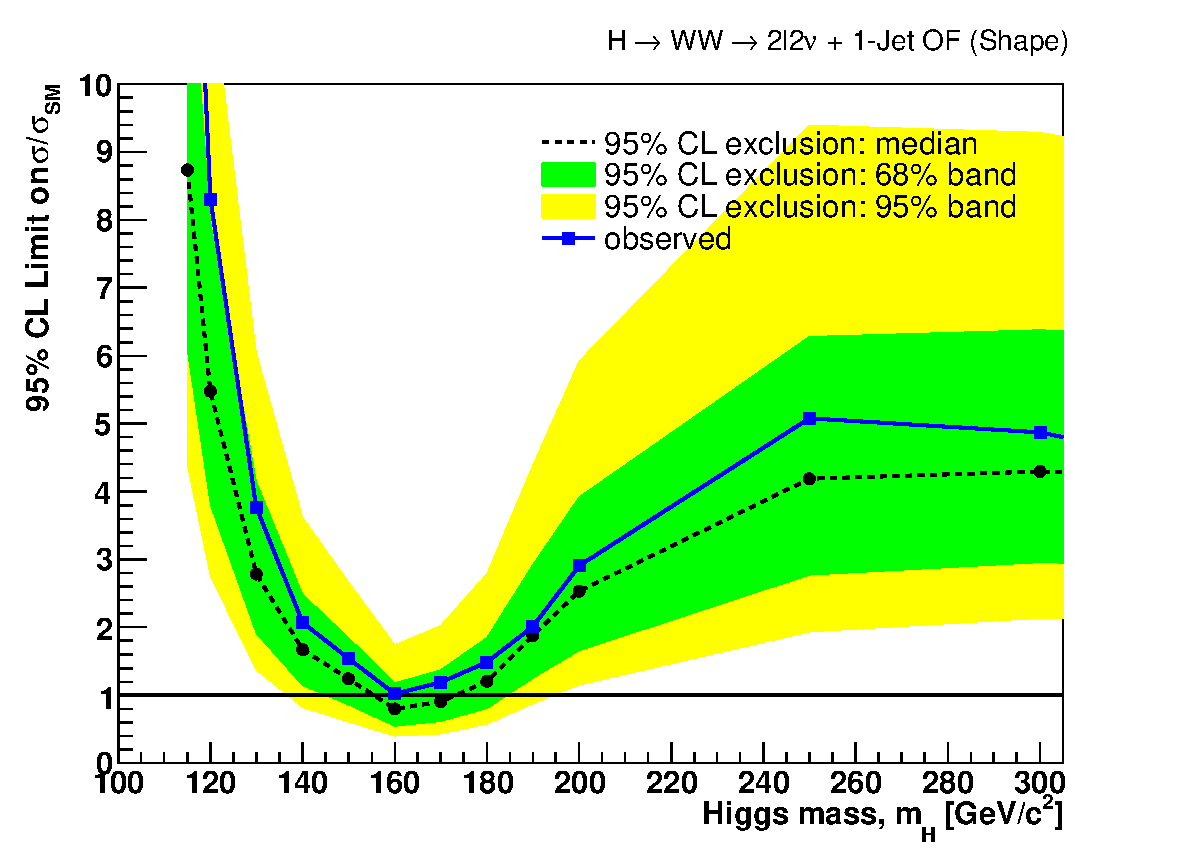
\includegraphics[width=0.48\textwidth]{lp_figures/limits_1j_of_shape_ana_v6_1500pb_LP_EPS.pdf}}
\subfigure[]{
\centering
\label{subfig:post_1j_sf_shape}
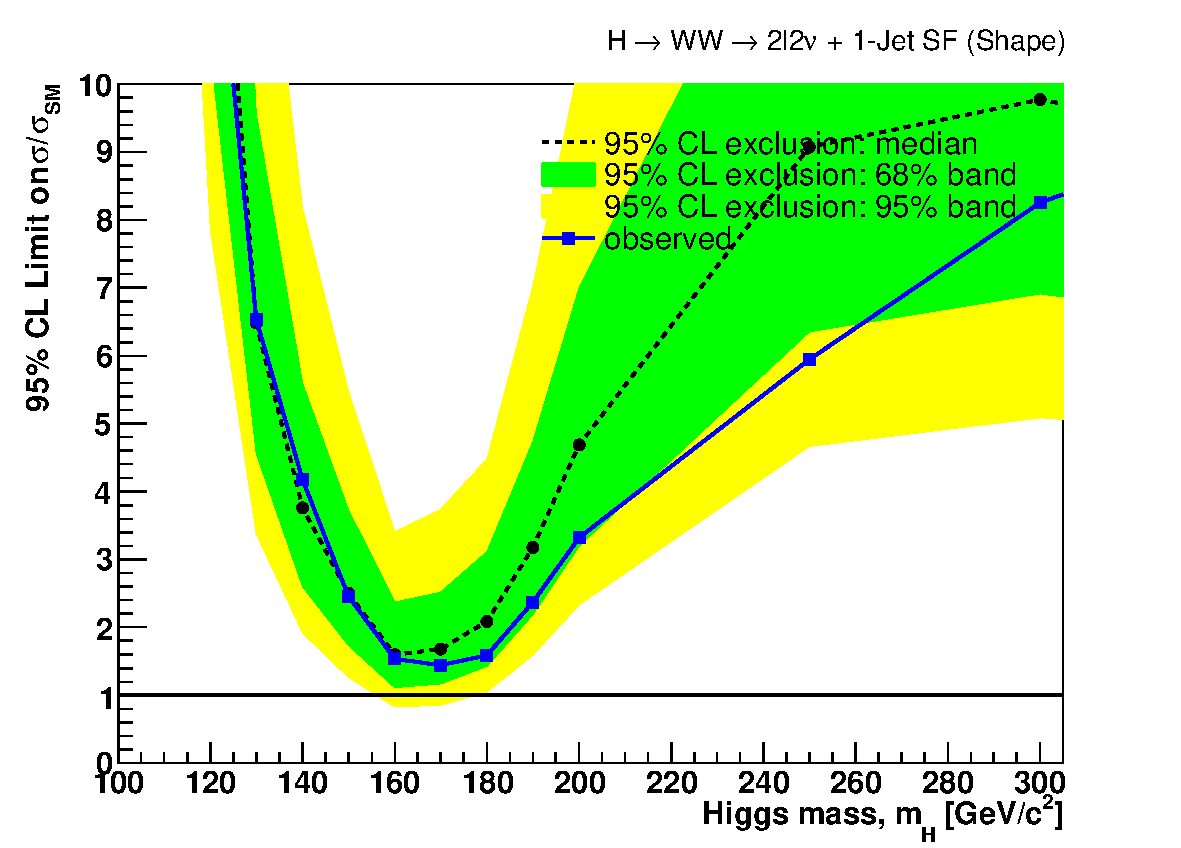
\includegraphics[width=0.48\textwidth]{lp_figures/limits_1j_sf_shape_ana_v6_1500pb_LP_POSTEPS.pdf}}
\subfigure[]{
\centering
\label{subfig:post_1j_of_shape}
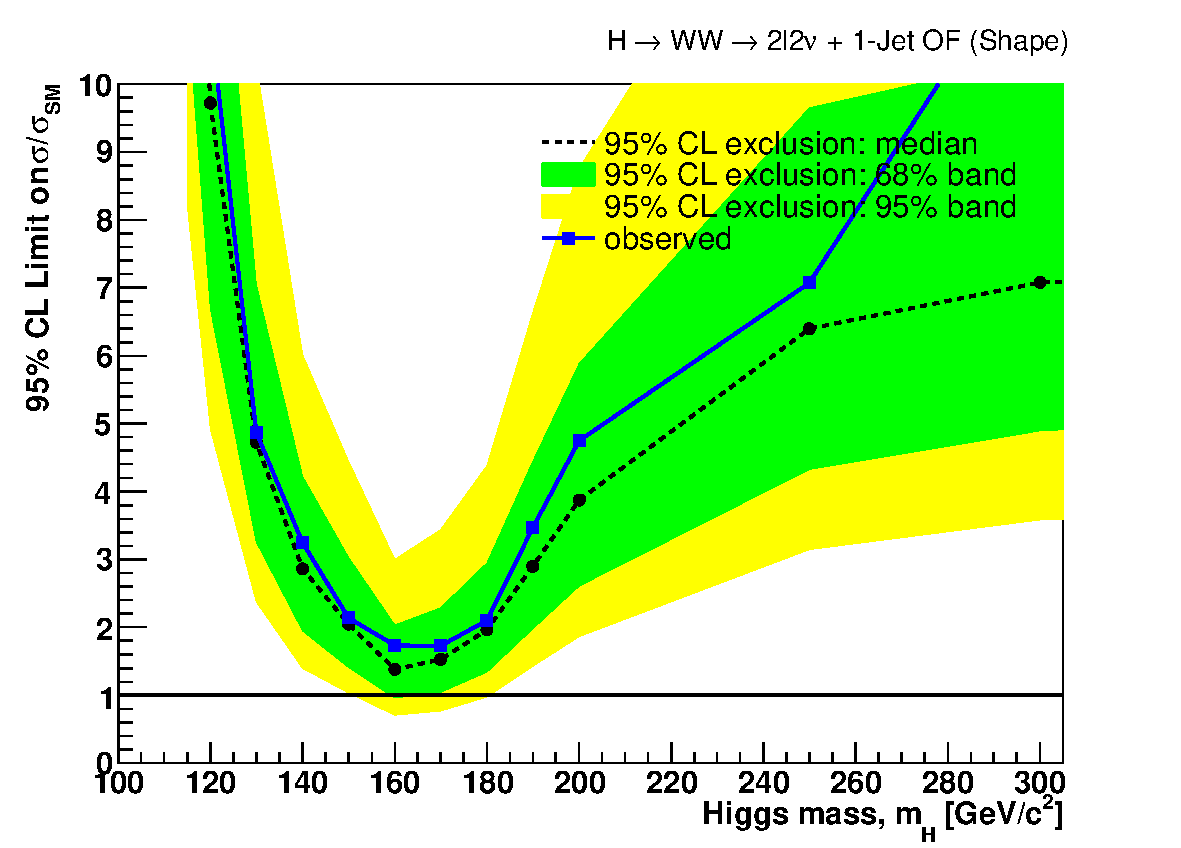
\includegraphics[width=0.48\textwidth]{lp_figures/limits_1j_of_shape_ana_v6_1500pb_LP_POSTEPS.pdf}}
\caption{Multivariate-based analysis upper limits at 95\% C.L. using LP, EPS and post-EPS datasets for 1-jet events.
\subref{subfig:lp_1j_sf_shape}: LP same-flavor; \subref{subfig:lp_1j_of_shape}: LP opposite-flavor; 
\subref{subfig:eps_1j_sf_shape}: EPS same-flavor; \subref{subfig:eps_1j_of_shape}: EPS opposite-flavor; 
\subref{subfig:post_1j_sf_shape}: post-EPS same-flavor; \subref{subfig:post_1j_of_shape}: post-EPS opposite-flavor; 
}
\label{fig:limits_1j_shape}
\end{figure}


%%%%%%%%%%%%%%%%%%%%%%%%%%%%%%
\begin{figure}[!htbp]
\centering
\subfigure[]{
\centering
\label{subfig:0j_sf}
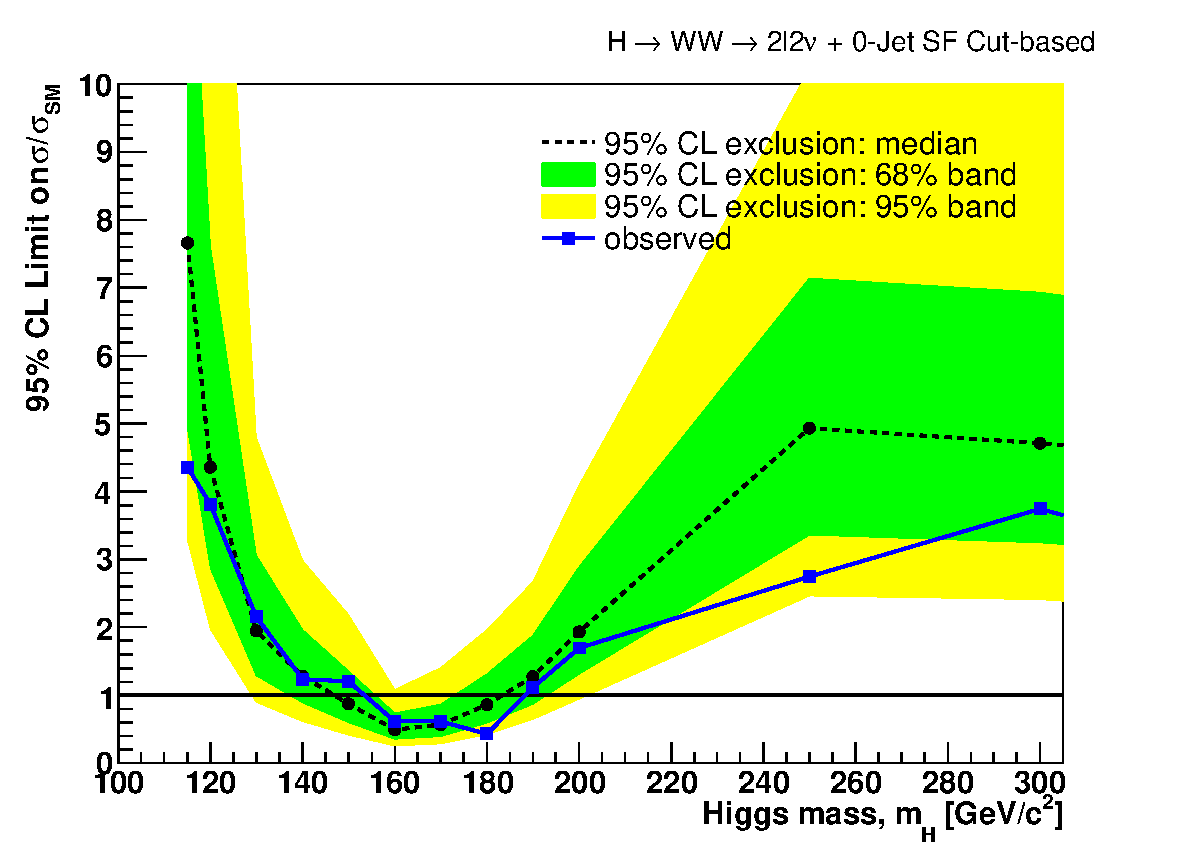
\includegraphics[width=0.48\textwidth]{lp_figures/limits_0j_sf_cut_ana_v6_1500pb_LP_MTCUT80.pdf}}
\subfigure[]{
\centering
\label{subfig:0j_of}
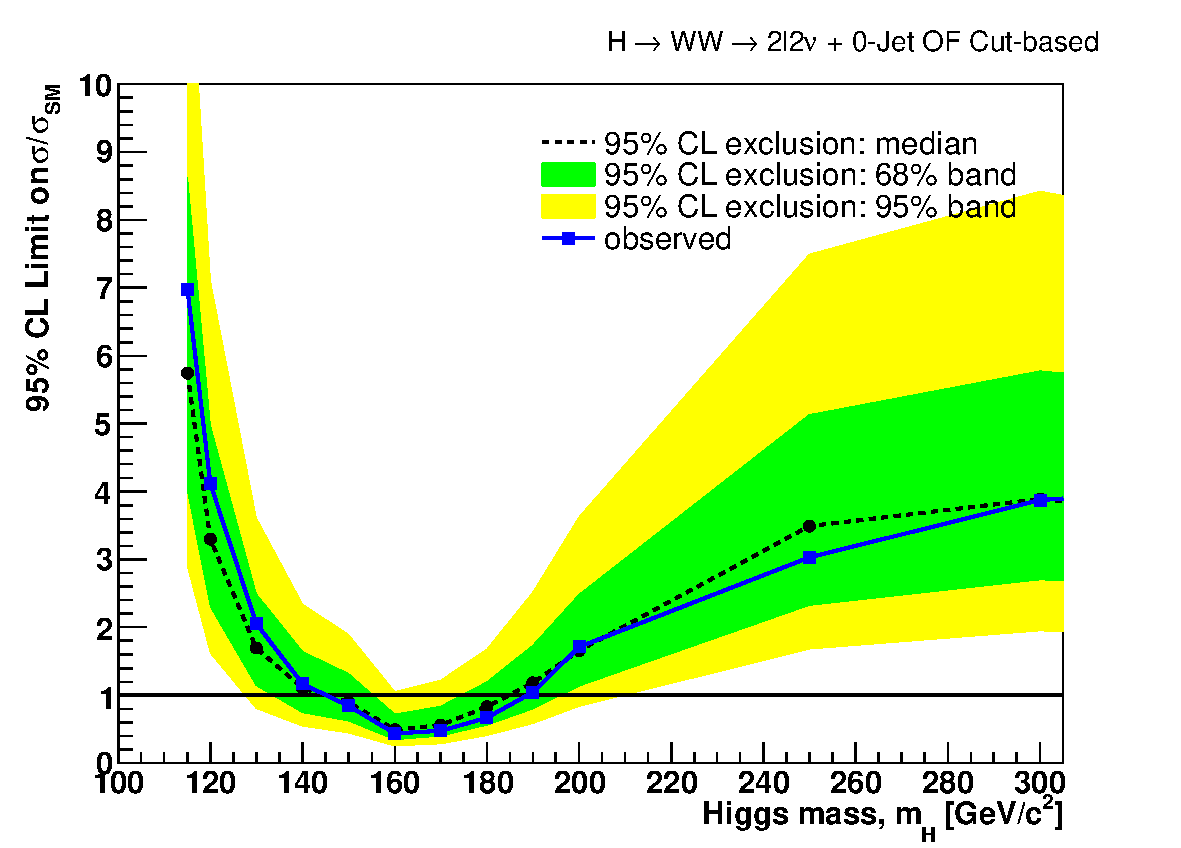
\includegraphics[width=0.48\textwidth]{lp_figures/limits_0j_of_cut_ana_v6_1500pb_LP_MTCUT80.pdf}}
\subfigure[]{
\centering
\label{subfig:1j_sf}
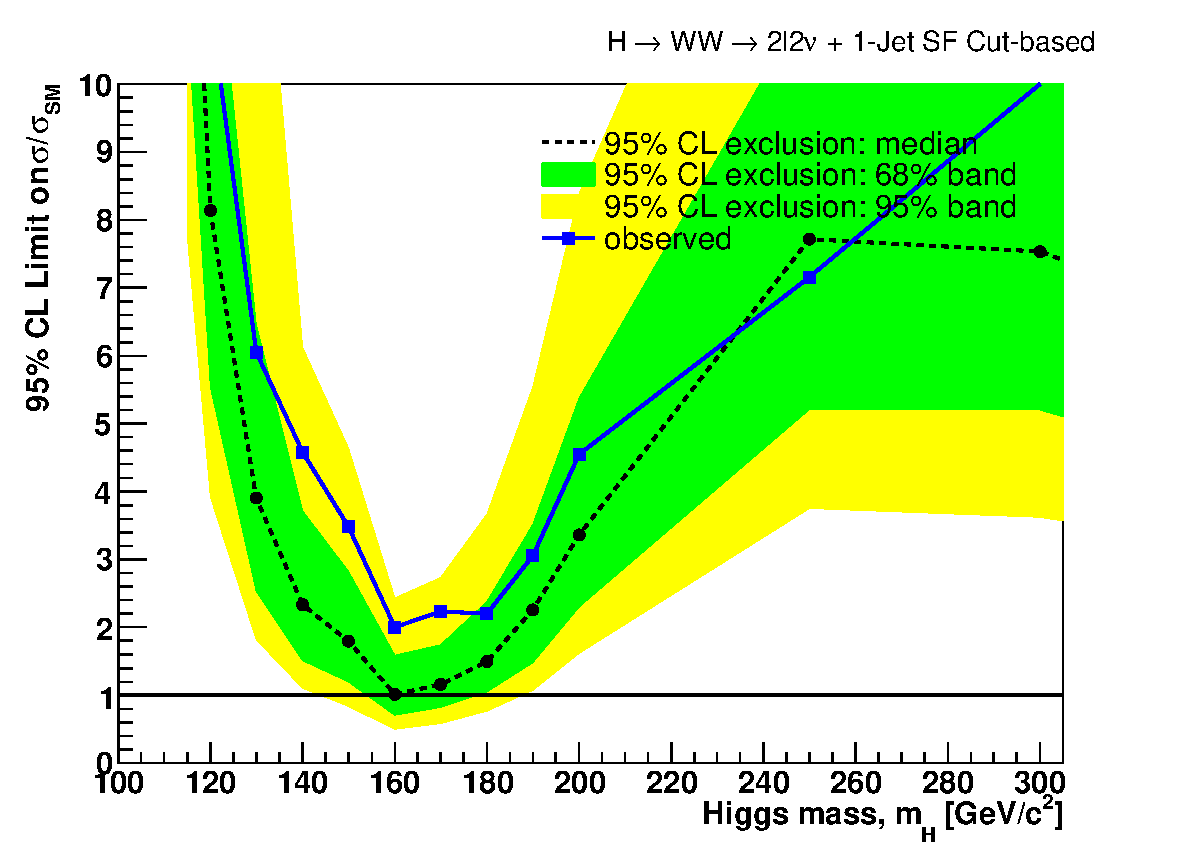
\includegraphics[width=0.48\textwidth]{lp_figures/limits_1j_sf_cut_ana_v6_1500pb_LP_MTCUT80.pdf}}
\subfigure[]{
\centering
\label{subfig:1j_of}
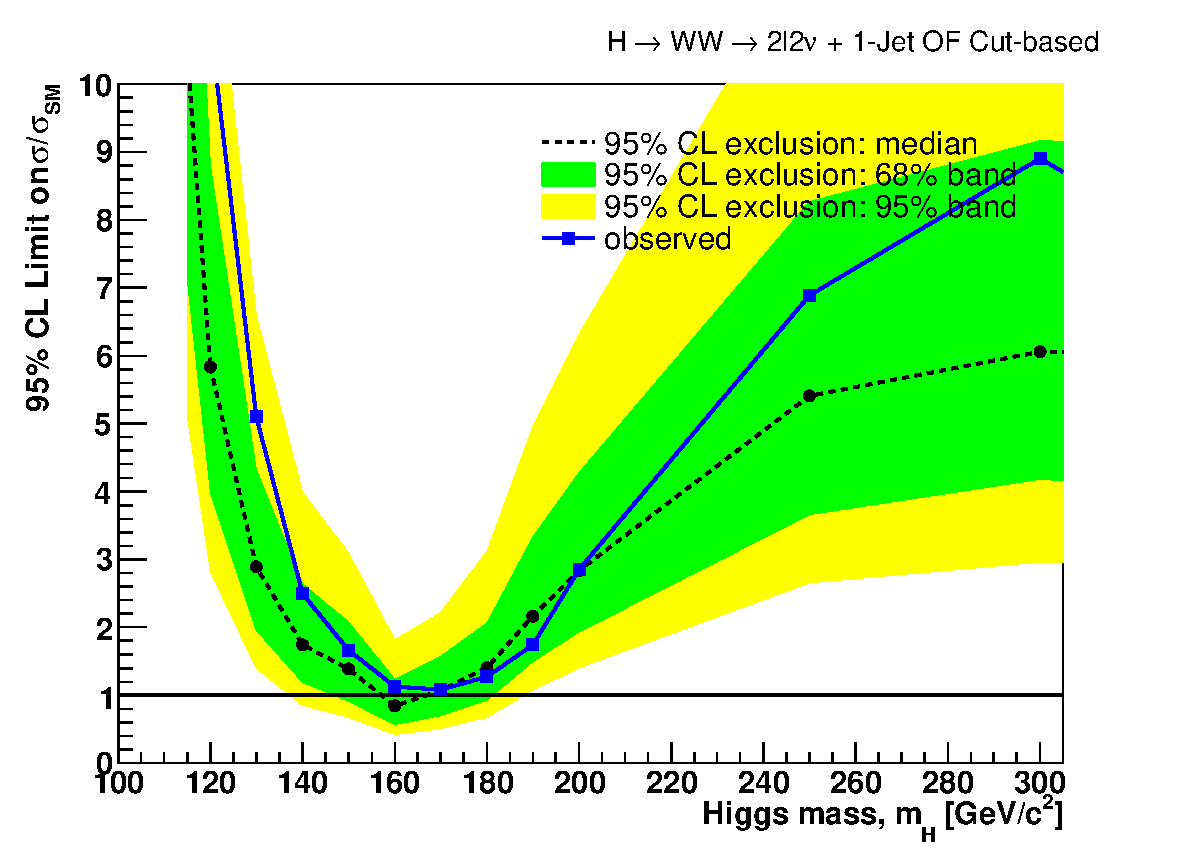
\includegraphics[width=0.48\textwidth]{lp_figures/limits_1j_of_cut_ana_v6_1500pb_LP_MTCUT80.pdf}}
\subfigure[]{
\centering
\label{subfig:2j}
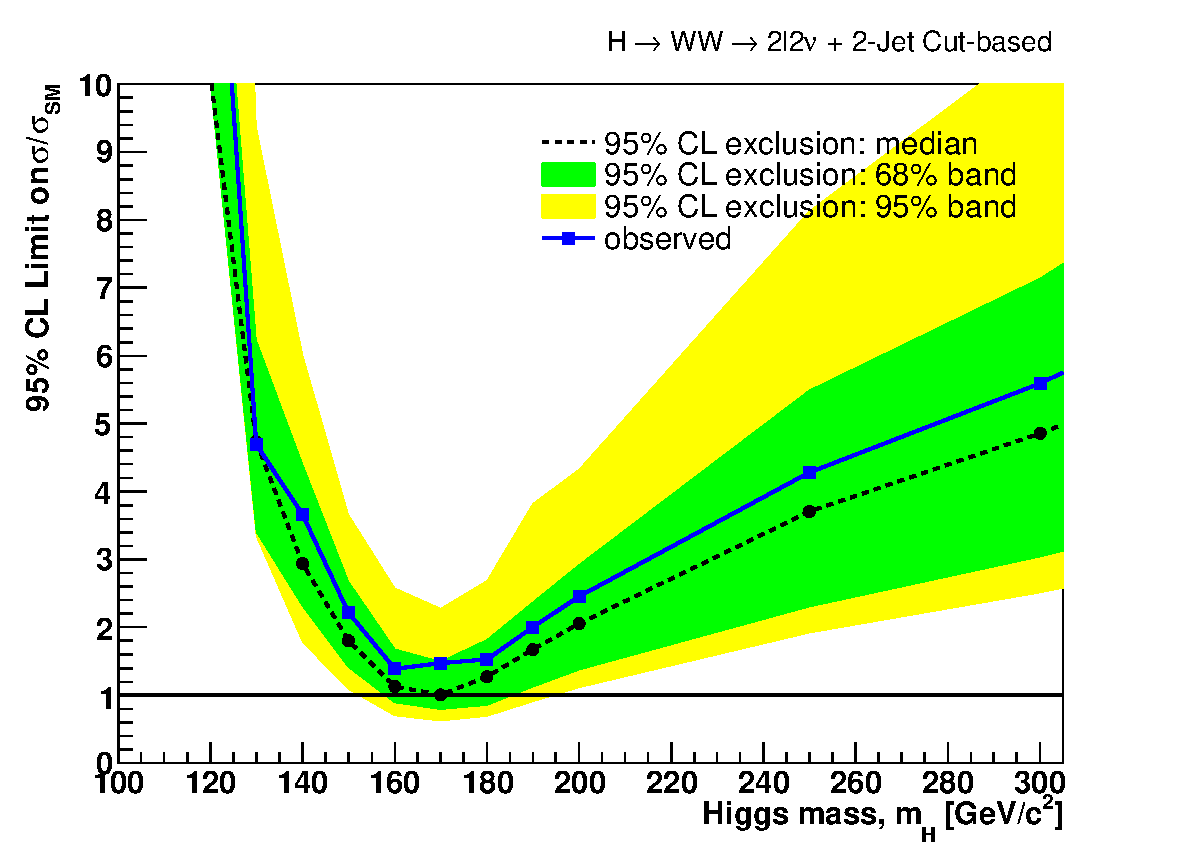
\includegraphics[width=0.48\textwidth]{lp_figures/limits_2j_cut_ana_v6_1500pb_LP_MTCUT80.pdf}}
\subfigure[]{
\centering
\label{subfig:njcomb}
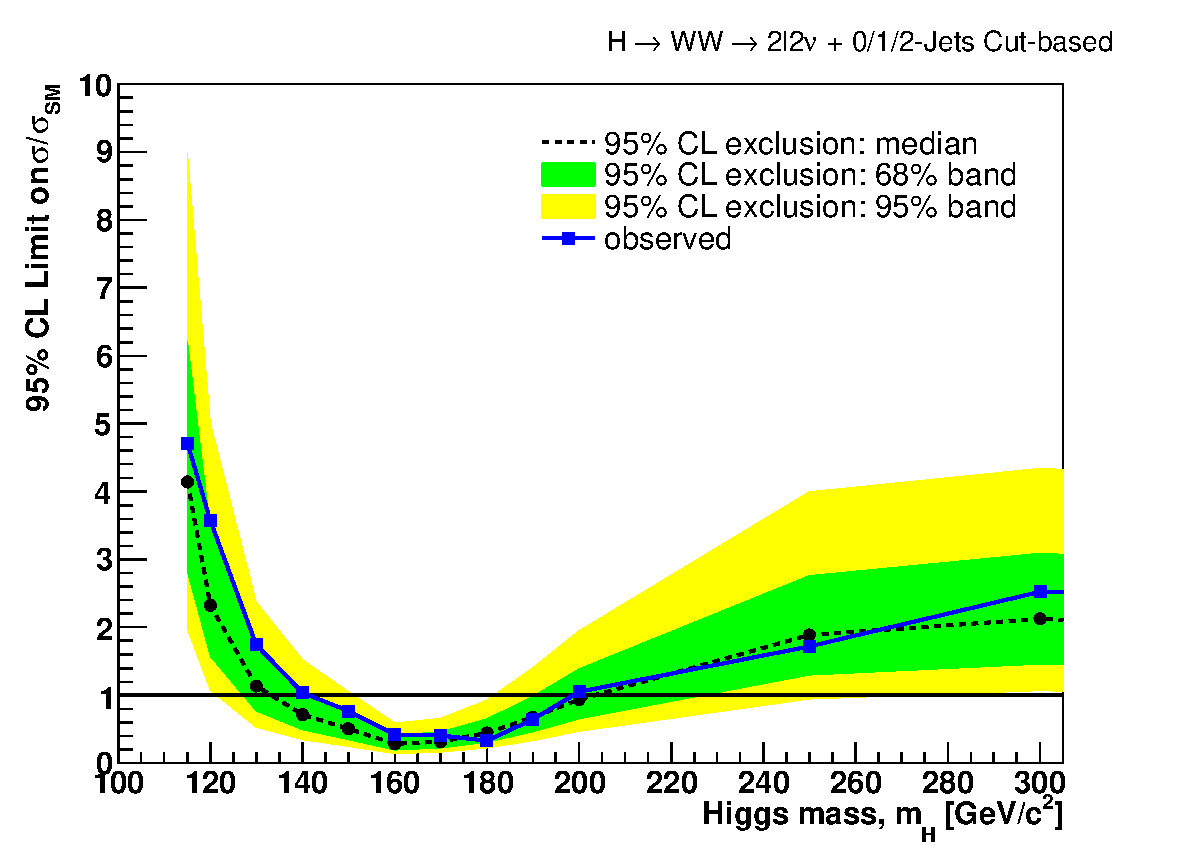
\includegraphics[width=0.48\textwidth]{lp_figures/limits_nj_cut_ana_v6_1500pb_LP_MTCUT80.pdf}}
\caption{Cut-based analysis upper limits at 95\% C.L. using data corresponding to 1.5~$\ifb$ applying the additional $m_T$ cut.
The limits are shown in 4 final states separately. \subref{subfig:0j_sf}: SF in 0 Jet bin; 
\subref{subfig:0j_of}: OF in 0 Jet bin; \subref{subfig:1j_sf}: SF in 1 Jet bin; 
\subref{subfig:1j_of}: OF in 1 Jet bin; \subref{subfig:2j}: 2 Jet bin; \subref{subfig:njcomb}: 0/1/2 Jets combined; }
\label{fig:limits_lp_mtcut80_cut}
\end{figure}
%%%%%%%%%%%%%%%%%%%%%%%%%%%%%%
%%%%%%%%%%%%%%%%%%%%%%%%%%%%%%
\begin{figure}[!htbp]
\centering
\subfigure[]{
\centering
\label{subfig:0j_sf}
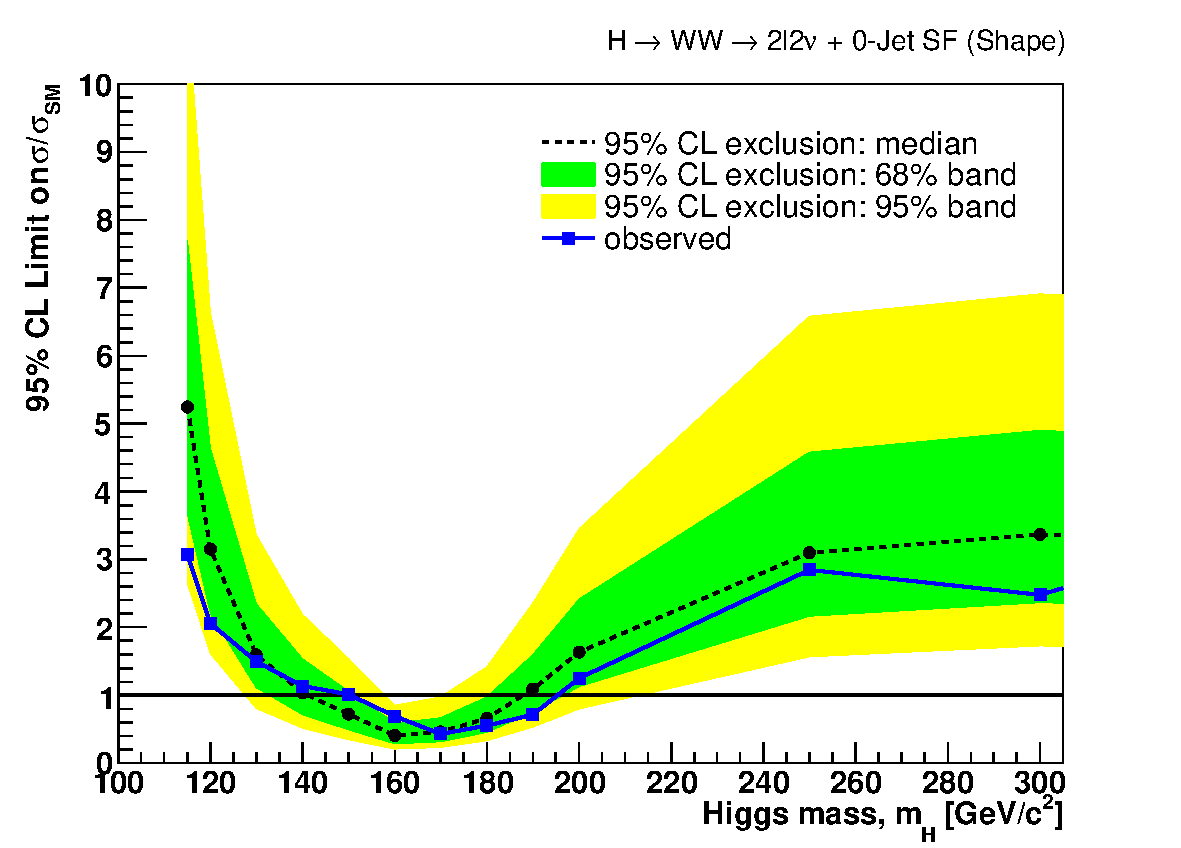
\includegraphics[width=0.48\textwidth]{lp_figures/limits_0j_sf_shape_ana_v6_1500pb_LP_MTCUT80.pdf}
}
\subfigure[]{
\centering
\label{subfig:0j_of}
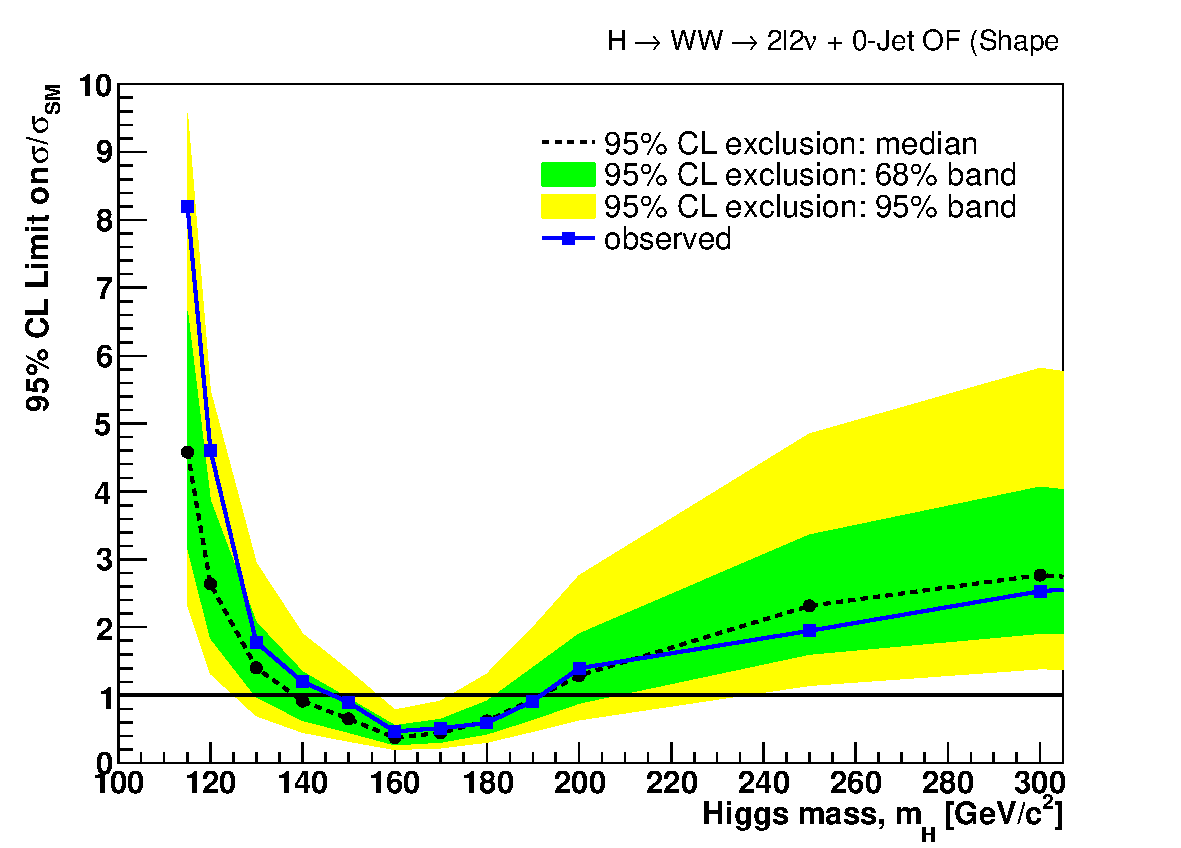
\includegraphics[width=0.48\textwidth]{lp_figures/limits_0j_of_shape_ana_v6_1500pb_LP_MTCUT80.pdf}
}
\subfigure[]{
\centering
\label{subfig:1j_sf}
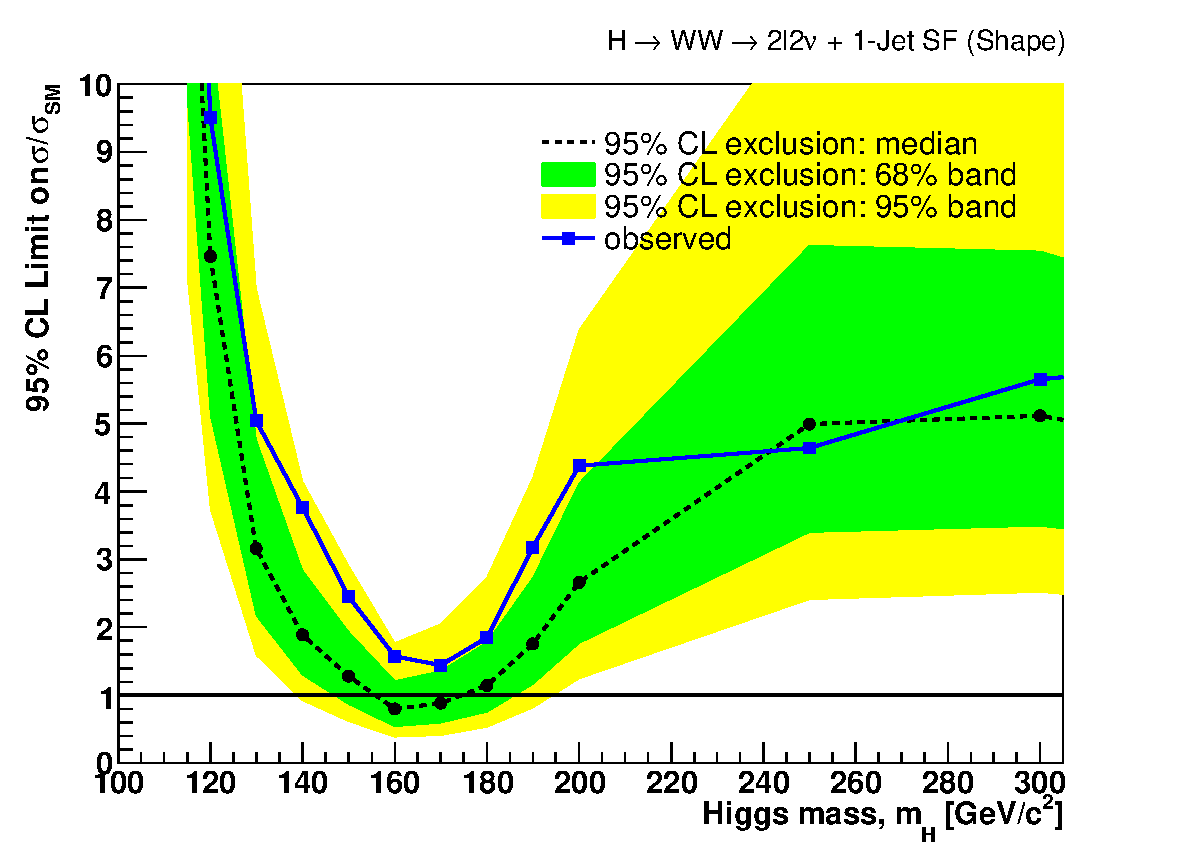
\includegraphics[width=0.48\textwidth]{lp_figures/limits_1j_sf_shape_ana_v6_1500pb_LP_MTCUT80.pdf}
}
\subfigure[]{
\centering
\label{subfig:1j_of}
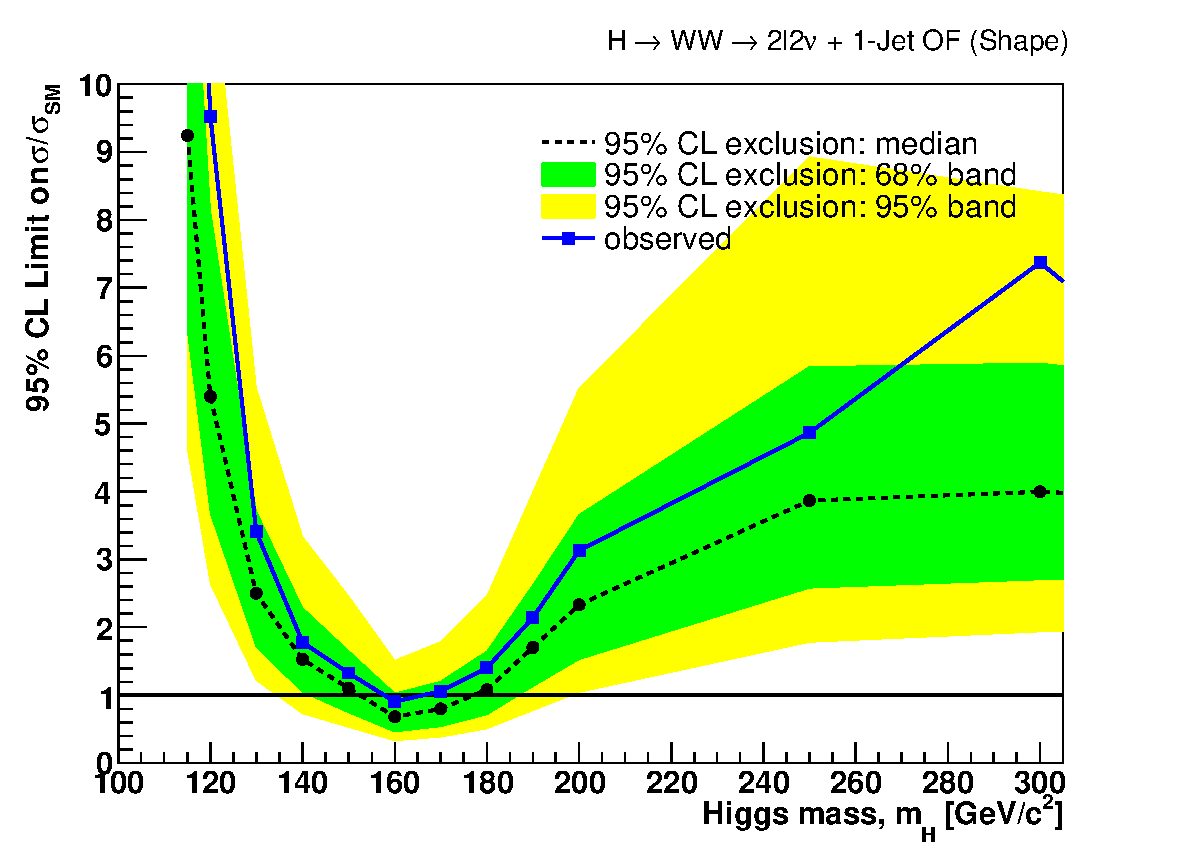
\includegraphics[width=0.48\textwidth]{lp_figures/limits_1j_of_shape_ana_v6_1500pb_LP_MTCUT80.pdf}
}
\subfigure[]{
\centering
\label{subfig:nj}
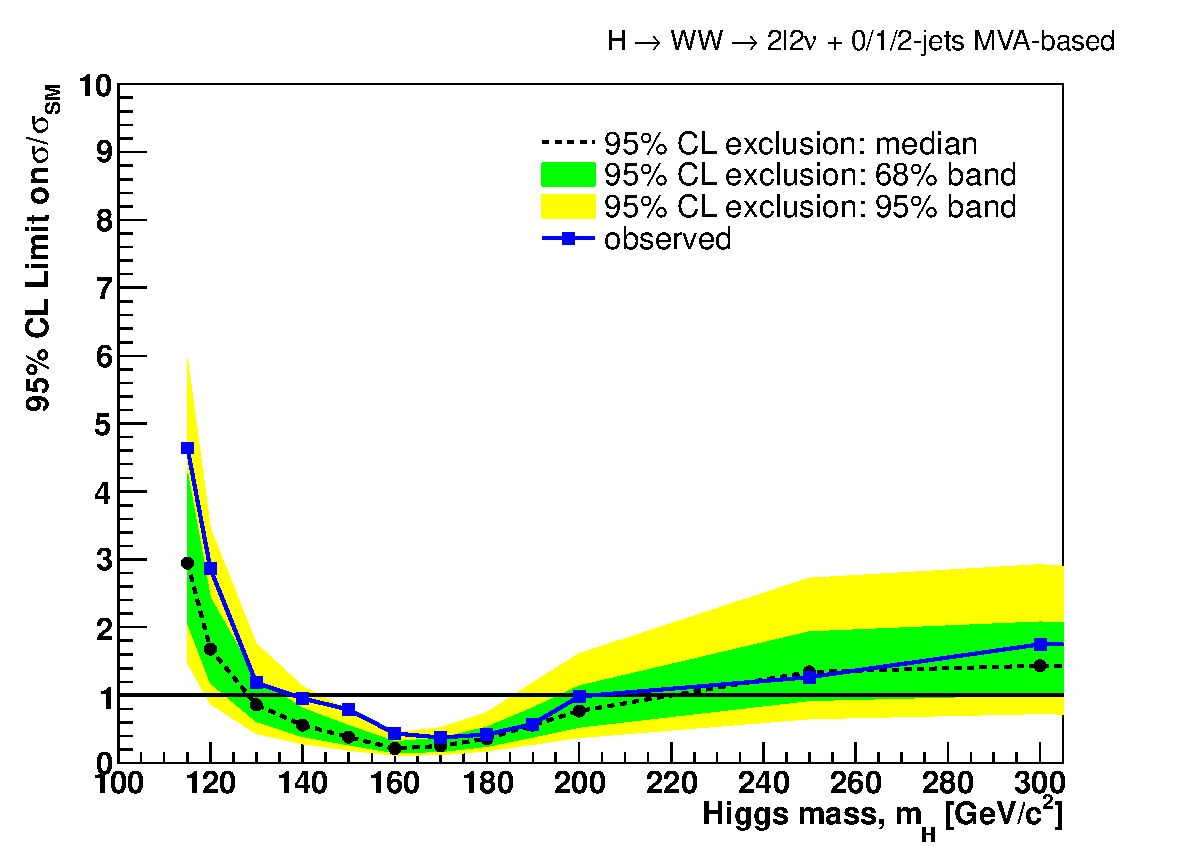
\includegraphics[width=0.48\textwidth]{lp_figures/limits_nj_shape_ana_v6_1500pb_LP_MTCUT80.pdf}
}
\caption{Multivariate based analysis upper limits at 95\% C.L. using data corresponding to 1.5~$\ifb$, 
applying the additional $m_T$ cut.
The limits are shown in 4 final states separately. \subref{subfig:0j_sf}: SF in 0 Jet bin; 
\subref{subfig:0j_of}: OF in 0 Jet bin; \subref{subfig:1j_sf}: SF in 1 Jet bin; 
\subref{subfig:1j_of}: OF in 1 Jet bin; \subref{subfig:nj}: 0/1/2 Jets combined;
}
\label{fig:limits_lp_mtcut80_shape}
\end{figure}
%%%%%%%%%%%%%%%%%%%%%%%%%%%%%%


\clearpage

\begin{table}[!ht]
\begin{center}
\begin{tabular} {c|ccc}
\hline
          & $10<p_T<15$ & $15<p_T<20$ & $p_T>20$ \\
\hline
\multicolumn{4}{c} {Barrel ($|\eta|<1.479$)} \\ \hline
post-EPS       & $0.3955 \pm 0.0411$ & $0.5443 \pm 0.0090$ & $0.6808 \pm 0.0029$ \\
EPS            & $0.4064 \pm 0.0250$ & $0.5184 \pm 0.0076$ & $0.6891 \pm 0.0013$ \\ \hline
\multicolumn{4}{c} {Endcap ($|\eta|>1.479$)} \\ \hline
post-EPS       & $0.1935 \pm 0.0265$ & $0.3320 \pm 0.0218$ & $0.6808 \pm 0.0029$ \\
EPS            & $0.2079 \pm 0.0103$ & $0.3219 \pm 0.0101$ & $0.6891 \pm 0.0013$ \\
\hline
\end{tabular}
\caption{Comparison of the electron efficiencies in the EPS and post-EPS datasets.}
\label{tab:lp_eff_electrons}
\end{center}
\end{table}

\begin{table}[!ht]
\begin{center}
\begin{tabular} {c|ccc}
\hline
          & $10<p_T<15$ & $15<p_T<20$ & $p_T>20$ \\
\hline
\multicolumn{4}{c} {Barrel ($|\eta|<1.479$)} \\ \hline
post-EPS       & N/A                 & $0.7651 \pm 0.0188$ & $0.6808 \pm 0.0029$ \\
EPS            & $0.6620 \pm 0.0108$ & $0.7306 \pm 0.0047$ & $0.6891 \pm 0.0013$ \\ \hline
\multicolumn{4}{c} {Endcap ($|\eta|>1.479$)} \\ \hline
post-EPS       & N/A                 & $0.7543 \pm 0.0197$ & $0.9193 \pm 0.0010$ \\
EPS            & $0.7079 \pm 0.0110$ & $0.7235 \pm 0.0073$ & $0.9138 \pm 0.0008$ \\
\hline
\end{tabular}
\caption{Comparison of the muon efficiencies in the EPS and post-EPS datasets.
Note that the low $p_T$ efficiencies were not available for the post-EPS dataset at the time of writing
with the code used to produce these results.
An independent measurement of the data to simulation scale factors found
$0.91 \pm 0.01$ ($0.91 \pm 0.02$) for the EPS dataset and $0.95 \pm 0.02$ ($0.90 \pm 0.03$)
for the post-EPS dataset in the Barrel (Endcap) regions.}
\label{tab:lp_eff_muons}
\end{center}
\end{table}

%===================================================================================================

%%%%%%%%%%%%%%%%%%%%%%%%%%%%%%
\begin{table}
\begin{center}
\begin{tabular}{c c c c c}
\hline
\vspace{-3mm} && \\
mass   & $N_{in}^{data}(DY)$ & $\langle R_{out/in} \rangle$ & $N_{out}^{data}(DY)$ & $N_{out}^{MC}(DY)$ \\
\vspace{-3mm} && \\
\hline
 WW & $ 26.02\pm15.19 $ & $ 0.25\pm0.06\pm0.03 $ & $ 6.39\pm4.02\pm0.82 $ & $ 2.11\pm0.44 $ \\\hline
 120 & $ 13.50\pm7.25 $ & $ 0.28\pm0.08\pm0.79 $ & $ 3.73\pm2.30\pm10.65 $ & $ 0.80\pm0.27 $ \\
 130 & $ 2.75\pm5.37 $ & $ 0.94\pm0.35\pm1.10 $ & $ 2.58\pm5.14\pm3.03 $ & $ 0.84\pm0.27 $ \\
 140 & $ 2.79\pm5.18 $ & $ 0.76\pm0.31\pm0.30 $ & $ 2.11\pm4.02\pm0.85 $ & $ 0.62\pm0.24 $ \\
 150 & $ 1.00\pm5.09 $ & $ 0.57\pm0.31\pm0.45 $ & $ 0.57\pm2.93\pm0.45 $ & $ 0.37\pm0.19 $ \\
 160 & $ 1.86\pm2.26 $ & $ 0.37\pm0.26\pm0.48 $ & $ 0.69\pm0.97\pm0.90 $ & $ 0.30\pm0.18 $ \\
 170 & $ 2.67\pm2.86 $ & $ 0.30\pm0.27\pm0.67 $ & $ 0.79\pm1.12\pm1.78 $ & $ 0.21\pm0.15 $ \\
 180 & $ 1.87\pm3.51 $ & $ 0.42\pm0.33\pm0.12 $ & $ 0.78\pm1.60\pm0.23 $ & $ 0.12\pm0.12 $ \\
 190 & $ 1.86\pm5.20 $ & $ 0.16\pm0.08\pm0.17 $ & $ 0.29\pm0.83\pm0.31 $ & $ 0.12\pm0.12 $ \\
 200 & $ 1.00\pm6.01 $ & $ 0.17\pm0.10\pm0.03 $ & $ 0.17\pm1.02\pm0.03 $ & $ 0.12\pm0.12 $ \\
 250 & $ 1.00\pm7.02 $ & $ 0.05\pm0.03\pm0.03 $ & $ 0.05\pm0.35\pm0.03 $ & $ 0.10\pm0.08 $ \\
 300 & $ 1.00\pm5.03 $ & $ 0.25\pm0.09\pm0.13 $ & $ 0.25\pm1.25\pm0.13 $ & $ 0.10\pm0.08 $ \\
\hline
\end{tabular}
\caption{The Drell-Yan estimation in the same flavor final state in the zero-jet bin.
\label{tab:routin_lp_data_0j}}
\end{center}
\end{table}
%%%%%%%%%%%%%%%%%%%%%%%%%%%%%%
%%%%%%%%%%%%%%%%%%%%%%%%%%%%%%
\begin{table}
\begin{center}
\begin{tabular}{c c c c c}
\hline
\vspace{-3mm} && \\
mass   & $N_{in}^{data}(DY)$ & $\langle R_{out/in} \rangle$ & $N_{out}^{data}(DY)$ & $N_{out}^{MC}(DY)$ \\
\vspace{-3mm} && \\
\hline
 WW & $ 67.24\pm12.67 $ & $ 0.14\pm0.03\pm0.07 $ & $ 9.62\pm2.52\pm4.38 $ & $ 3.42\pm0.58 $ \\\hline
 120 & $ 25.72\pm5.49 $ & $ 0.08\pm0.02\pm0.17 $ & $ 1.93\pm0.67\pm4.31 $ & $ 1.05\pm0.34 $ \\
 130 & $ 11.64\pm4.14 $ & $ 0.09\pm0.03\pm0.35 $ & $ 1.05\pm0.49\pm4.02 $ & $ 0.86\pm0.31 $ \\
 140 & $ 11.34\pm4.15 $ & $ 0.09\pm0.03\pm0.24 $ & $ 0.98\pm0.47\pm2.68 $ & $ 0.94\pm0.32 $ \\
 150 & $ 22.78\pm5.59 $ & $ 0.06\pm0.02\pm0.11 $ & $ 1.40\pm0.66\pm2.57 $ & $ 0.59\pm0.25 $ \\
 160 & $ 7.05\pm4.04 $ & $ 0.19\pm0.08\pm0.21 $ & $ 1.31\pm0.94\pm1.45 $ & $ 0.58\pm0.25 $ \\
 170 & $ 5.98\pm3.91 $ & $ 0.19\pm0.08\pm0.15 $ & $ 1.14\pm0.89\pm0.88 $ & $ 0.27\pm0.13 $ \\
 180 & $ 3.42\pm3.92 $ & $ 0.15\pm0.06\pm0.11 $ & $ 0.51\pm0.62\pm0.38 $ & $ 0.26\pm0.13 $ \\
 190 & $ 15.24\pm5.62 $ & $ 0.08\pm0.03\pm0.13 $ & $ 1.27\pm0.65\pm1.99 $ & $ 0.32\pm0.14 $ \\
 200 & $ 24.38\pm6.85 $ & $ 0.06\pm0.02\pm0.09 $ & $ 1.54\pm0.71\pm2.19 $ & $ 0.32\pm0.14 $ \\
 250 & $ 32.75\pm7.85 $ & $ 0.07\pm0.02\pm0.01 $ & $ 2.26\pm0.88\pm0.40 $ & $ 0.62\pm0.23 $ \\
 300 & $ 25.46\pm6.48 $ & $ 0.06\pm0.02\pm0.07 $ & $ 1.42\pm0.70\pm1.75 $ & $ 0.40\pm0.19 $ \\
\hline
\end{tabular}
\caption{The Drell-Yan estimation in the same flavor final state in the one-jet bin.
\label{tab:routin_lp_data_1j}}
\end{center}
\end{table}
%%%%%%%%%%%%%%%%%%%%%%%%%%%%%%

\begin{table}[!htbp]
\begin{center}
\begin{tabular}{c c c c} 
\hline
Period & 0-jet bin & 1-jet bin & 2-jet bin \\ 
\hline
EPS      & 3.47 $\pm$ 2.26 & 2.69 $\pm$ 1.37 & 4.81 $\pm$ 1.84 \\
post-EPS & 2.71 $\pm$ 3.50 & 3.17 $\pm$ 1.84 & 4.90 $\pm$ 1.97 \\
LP       & 3.02 $\pm$ 1.84 & 2.81 $\pm$ 1.40 & 4.84 $\pm$ 1.83 \\
\hline
\end{tabular}
\caption{Comparison of data to simulation scale factors for the DY background for the EPS, post-EPS and LP datasets.}
\label{tab:lp_periods_dy}
\end{center}
\end{table}

\begin{table}[!htbp]
\begin{center}
\begin{tabular}{c c c c c c} 
\hline
jet-bin &	 $\mu\mu$ &	 $\mu e$ &	 $e\mu$ &	 $ee$ &	 total \\ 
\hline
0 &	 12.76 $\pm$ 2.24 &	 43.67 $\pm$ 2.72 &	 66.67 $\pm$ 4.22 &	 15.34 $\pm$ 1.47 &	 138.46 $\pm$ 5.69 \\
1 &	 6.70 $\pm$ 1.86  &      16.45 $\pm$ 1.87 &      28.18 $\pm$ 2.86 &       4.91 $\pm$ 0.93 &       56.27 $\pm$ 4.00 \\
2 &	 2.04 $\pm$ 1.26  &       2.85 $\pm$ 0.61 &      13.39 $\pm$ 1.90 &       1.42 $\pm$ 0.55 &       22.62 $\pm$ 2.66 \\
\hline
\end{tabular}
\caption{Predictions of the fake-induced background contribution 
in the data-driven estimation after the $WW$ preselection. 
The analyzed data correspond to \lpintlumi.
The uncertainties are statistical only.}
\label{tab:lp_fake_est}
\end{center}
\end{table}

\begin{table}[!htbp]
\begin{center}
\begin{tabular}{c c c c}
\hline
Period & 0-jet bin & 1-jet bin & 2-jet bin \\
\hline
EPS      & 94.4 $\pm$ 4.4 & 34.2 $\pm$ 2.9 & 13.9 $\pm$ 1.9 \\
post-EPS & 76.5 $\pm$ 6.3 & 42.6 $\pm$ 5.3 & 16.9 $\pm$ 3.6 \\
LP       & 89.6 $\pm$ 3.7 & 36.4 $\pm$ 2.6 & 14.6 $\pm$ 1.7 \\
\hline
\end{tabular}
\caption{Comparison of the number of fake-induced events per \ifb~of data in the EPS, post-EPS and LP datasets.}
\label{tab:lp_periods_fake}
\end{center}
\end{table}

\begin{table}[!htbp]
\begin{center}
\begin{tabular}{|l|c|c|}
\hline
Type                                                             & Yield \\
\hline
Estimated events                                                 &  $68.4\pm3.8^{+15.6}_{-10.6}$  \\
\hline
Observed same-sign events in Data                                &  $92$        \\
Monte Carlo estimate of non-fake contribution (WZ \& W$\gamma)$  & $28.0\pm1.9$ \\
Fake background observed                                         & $64.0\pm9.7$ \\
\hline
\end{tabular}
\caption{Summary of fake lepton background yields in the same sign sample after WW selection (\lpintlumi). }
\label{tab:lp_FakeLeptonBkgPrediction_SameSignSample}
\end{center}
\end{table}

\begin{table}[!htbp]
\begin{center}
\begin{tabular}{l c c c}
\hline
Sample                                        &   0-jet          & 1-jet          \\
\hline
Estimated top events in simulation  	      &  48.1 $\pm$ 2.9  & 147.8 $\pm$ 4.4 \\
tagging efficiency (\%)                       &  52.5 $\pm$ 4.6  &  68.1 $\pm$ 1.6 \\
top-tagged events in data           	      &          106     &    386          \\
background events in control region           &  26.3 $\pm$ 4.6  &  21.1 $\pm$ 3.7 \\
Data-driven top background estimate           &  72.1 $\pm$ 17.5 & 170.5 $\pm$ 15.3\\
\hline
\end{tabular}
\caption{Predictions of the top background contribution compared 
with observed event counts in the data-driven estimation after the $WW$ preselection. 
The analyzed data correspond to \lpintlumi.
The uncertainties are statistical only. The systematic uncertainties are expected to be 
negligible at this level or precision.}
\label{tab:lp_ttbar_est}
\end{center}
\end{table}

\begin{table}[!htbp]
\begin{center}
\begin{tabular}{c c c} 
\hline
Period & 0-jet bin & 1-jet bin \\ 
\hline
EPS      & 1.67 $\pm$ 0.25 & 1.20 $\pm$ 0.10 \\
post-EPS & 1.12 $\pm$ 0.40 & 1.02 $\pm$ 0.18 \\
LP       & 1.50 $\pm$ 0.24 & 1.15 $\pm$ 0.09 \\
\hline
\end{tabular}
\caption{Comparison of data to simulation scale factors for the top background for the EPS, post-EPS and LP datasets.}
\label{tab:lp_periods_top}
\end{center}
\end{table}

\begin{table}[!htbp]
\begin{center}
\begin{tabular}{c | c c c | c c c}
\hline
$m_H$ & \multicolumn{3}{c}{0-jet bin} & \multicolumn{3}{|c}{1-jet bin} \\
$[\GeVcc]$ & estimate & expected & scale factor & estimate  & expected & scale factor \\ \hline
115 & 46.6 $\pm$  5.3 & 43.7 $\pm$  0.7 & 1.07 $\pm$ 0.12 & 10.9 $\pm$  2.9 &  9.9 $\pm$  0.3 & 1.11 $\pm$ 0.29 \\
120 & 61.0 $\pm$  6.9 & 57.2 $\pm$  0.8 & 1.07 $\pm$ 0.12 & 14.4 $\pm$  3.8 & 13.0 $\pm$  0.4 & 1.11 $\pm$ 0.29 \\
130 & 70.5 $\pm$  8.0 & 65.8 $\pm$  0.8 & 1.07 $\pm$ 0.12 & 16.7 $\pm$  4.4 & 15.0 $\pm$  0.4 & 1.11 $\pm$ 0.29 \\
140 & 64.1 $\pm$  7.2 & 60.9 $\pm$  0.8 & 1.05 $\pm$ 0.12 & 15.1 $\pm$  3.9 & 13.6 $\pm$  0.4 & 1.11 $\pm$ 0.29 \\
150 & 41.3 $\pm$  5.0 & 42.0 $\pm$  0.6 & 0.98 $\pm$ 0.12 & 13.3 $\pm$  3.6 & 12.2 $\pm$  0.3 & 1.09 $\pm$ 0.30 \\
160 & 28.7 $\pm$  3.5 & 29.2 $\pm$  0.5 & 0.99 $\pm$ 0.12 & 11.3 $\pm$  3.1 & 10.4 $\pm$  0.3 & 1.09 $\pm$ 0.30 \\
170 & 22.7 $\pm$  2.8 & 23.0 $\pm$  0.5 & 0.98 $\pm$ 0.12 &  9.5 $\pm$  2.6 &  8.7 $\pm$  0.3 & 1.10 $\pm$ 0.30 \\
180 & 26.0 $\pm$  3.2 & 26.5 $\pm$  0.5 & 0.98 $\pm$ 0.12 & 11.5 $\pm$  3.1 & 10.3 $\pm$  0.3 & 1.12 $\pm$ 0.30 \\
190 & 39.5 $\pm$  4.7 & 39.9 $\pm$  0.6 & 0.99 $\pm$ 0.12 & 16.7 $\pm$  4.4 & 14.9 $\pm$  0.4 & 1.12 $\pm$ 0.30 \\
200 & 40.6 $\pm$  4.9 & 41.5 $\pm$  0.6 & 0.98 $\pm$ 0.12 & 18.7 $\pm$  4.9 & 16.5 $\pm$  0.4 & 1.14 $\pm$ 0.30 \\
\hline
\end{tabular}
\caption{Cut-based analysis: data driven WW estimation for different Higgs masses in the 0- and 1-jet bins (\lpintlumi). 
Only statistical uncertainties are reported.}
\label{tab:lp_wwEstimResData}
\end{center}
\end{table}

\begin{table}[!htbp]
\begin{center}
\begin{tabular}{c | c c c | c c c}
\hline
$m_H$ & \multicolumn{3}{c}{0-jet bin} & \multicolumn{3}{|c}{1-jet bin} \\
$[\GeVcc]$ & estimate & expected & scale factor & estimate  & expected & scale factor \\ \hline
115 & 274.9 $\pm$ 31.1 & 257.8 $\pm$  1.6 & 1.07 $\pm$ 0.12 & 84.8 $\pm$ 22.3 & 76.8 $\pm$  0.9 & 1.11 $\pm$ 0.29 \\
120 & 274.9 $\pm$ 31.1 & 257.8 $\pm$  1.6 & 1.07 $\pm$ 0.12 & 84.8 $\pm$ 22.3 & 76.8 $\pm$  0.9 & 1.11 $\pm$ 0.29 \\
130 & 317.4 $\pm$ 35.9 & 297.6 $\pm$  1.7 & 1.07 $\pm$ 0.12 & 98.8 $\pm$ 26.0 & 89.4 $\pm$  0.9 & 1.11 $\pm$ 0.29 \\
140 & 344.9 $\pm$ 39.0 & 323.4 $\pm$  1.8 & 1.07 $\pm$ 0.12 & 107.5 $\pm$ 28.3 & 97.3 $\pm$  1.0 & 1.11 $\pm$ 0.29 \\
150 & 368.4 $\pm$ 41.7 & 345.5 $\pm$  1.8 & 1.07 $\pm$ 0.12 & 114.5 $\pm$ 30.1 & 103.6 $\pm$  1.0 & 1.11 $\pm$ 0.29 \\
160 & 368.4 $\pm$ 41.7 & 345.5 $\pm$  1.8 & 1.07 $\pm$ 0.12 & 114.5 $\pm$ 30.1 & 103.6 $\pm$  1.0 & 1.11 $\pm$ 0.29 \\
170 & 368.4 $\pm$ 41.7 & 345.5 $\pm$  1.8 & 1.07 $\pm$ 0.12 & 114.5 $\pm$ 30.1 & 103.6 $\pm$  1.0 & 1.11 $\pm$ 0.29 \\
180 & 392.4 $\pm$ 44.4 & 368.0 $\pm$  1.9 & 1.07 $\pm$ 0.12 & 122.2 $\pm$ 32.1 & 110.6 $\pm$  1.0 & 1.11 $\pm$ 0.29 \\
190 & 417.6 $\pm$ 47.2 & 391.6 $\pm$  2.0 & 1.07 $\pm$ 0.12 & 130.9 $\pm$ 34.4 & 118.5 $\pm$  1.1 & 1.11 $\pm$ 0.29 \\
200 & 438.2 $\pm$ 49.5 & 410.9 $\pm$  2.0 & 1.07 $\pm$ 0.12 & 137.4 $\pm$ 36.1 & 124.3 $\pm$  1.1 & 1.11 $\pm$ 0.29 \\\hline
\end{tabular}
\caption{MVA analysis: data driven WW estimation for different Higgs masses in the 0- and 1-jet bin (\lpintlumi). 
Only statistical uncertainties are reported.}
\label{tab:lp_wwEstimResDataMVA}
\end{center}
\end{table}

\begin{table}[!htbp]
\begin{center}
\begin{tabular}{c c c} 
\hline
Period & 0-jet bin & 1-jet bin \\ 
\hline
EPS      & 1.05 $\pm$ 0.14 & 1.14 $\pm$ 0.33 \\
post-EPS & 1.09 $\pm$ 0.20 & 1.00 $\pm$ 0.51 \\
LP       & 1.07 $\pm$ 0.12 & 1.11 $\pm$ 0.29 \\
\hline
\end{tabular}
\caption{Comparison of data to simulation scale factors for the WW background (MVA analysis) for the EPS, post-EPS and LP datasets.}
\label{tab:lp_periods_ww}
\end{center}
\end{table}

\clearpage


\appendix

\section{Data Validation Plots}
\label{app:lp_postEPSdist}
Plots are normalized to 1$/fb$. 
Error bars are the sum in quadrature of the statistical uncertainty of EPS and post-EPS data. 
EPS dataset corresponds to run$<$170826, post-EPS to run$\geq$170826.

\clearpage

\begin{figure}[!hbtp]
\centering
\subfigure[]{
\centering
\label{subfig:lp_dPhi_ww0j}
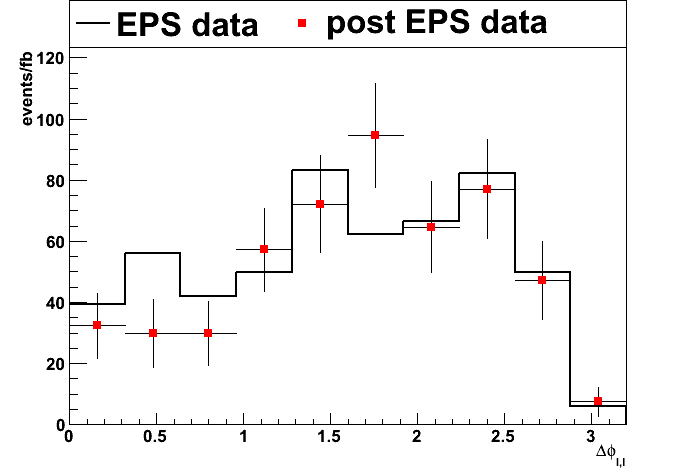
\includegraphics[width=.32\textwidth]{lp_figures/postEPSvalid/hm0/dPhi_ww0j.png}}
\subfigure[]{
\centering
\label{subfig:lp_dilepmass_ww0j}
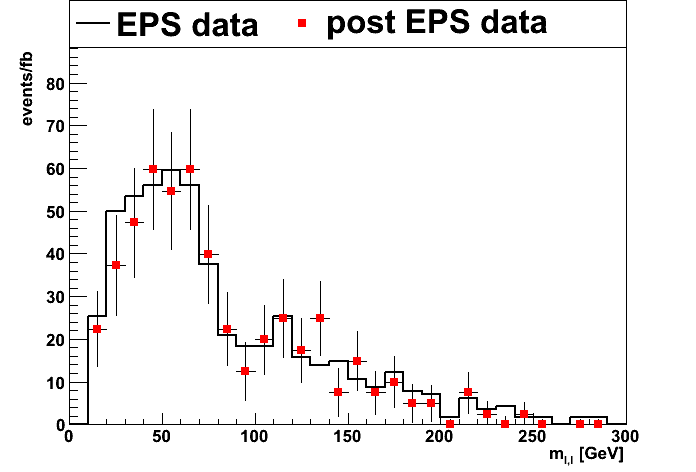
\includegraphics[width=.32\textwidth]{lp_figures/postEPSvalid/hm0/dilepmass_ww0j.png}}\\
\subfigure[]{
\centering
\label{subfig:lp_dileppt_ww0j}
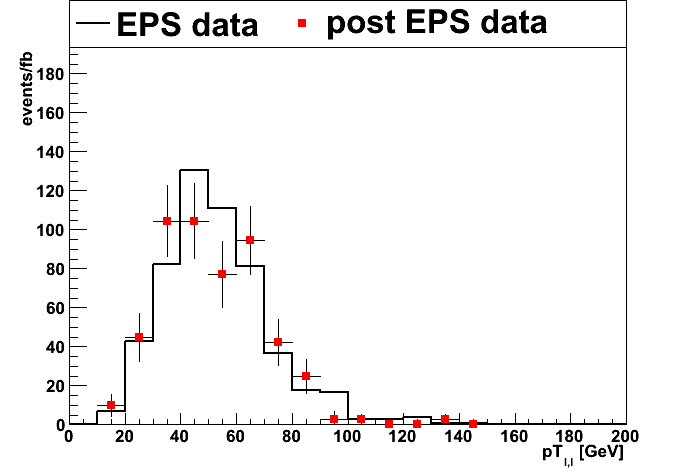
\includegraphics[width=.32\textwidth]{lp_figures/postEPSvalid/hm0/dileppt_ww0j.png}}
\subfigure[]{
\centering
\label{subfig:lp_type_ww0j}
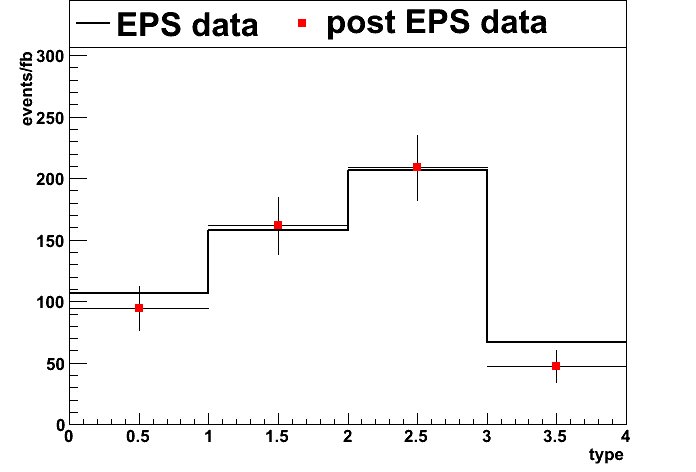
\includegraphics[width=.32\textwidth]{lp_figures/postEPSvalid/hm0/type_ww0j.png}}
\caption{EPS and post-EPS data comparison: 0-jet bin, all final states. 
\subref{subfig:lp_dPhi_ww0j} $\Delta\phi$ between the two leptons;
\subref{subfig:lp_dilepmass_ww0j} di-lepton invariant mass;
\subref{subfig:lp_dileppt_ww0j} di-lepton transverse momentum;
\subref{subfig:lp_type_ww0j} di-lepton type ($\mu\mu$=0, $\mu e$=2, $e\mu$=2, $ee$=3).
}
\label{fig:lp_ww0j_dilep}
\end{figure}

\begin{figure}[!hbtp]
\centering
\subfigure[]{
\centering
\label{subfig:lp_lep1pt_ww0j}
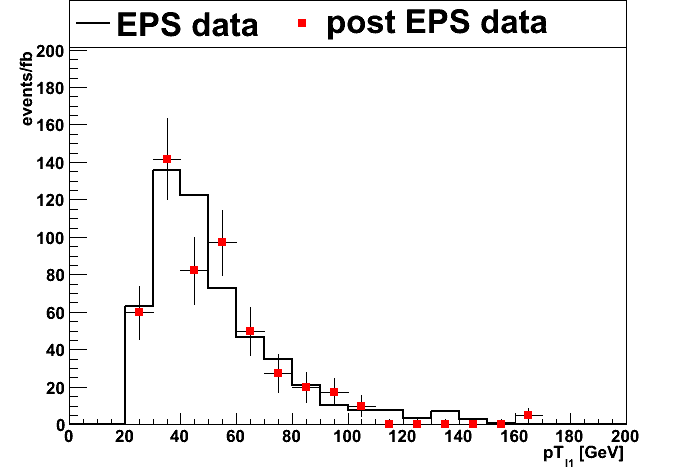
\includegraphics[width=.32\textwidth]{lp_figures/postEPSvalid/hm0/lep1pt_ww0j.png}}
\subfigure[]{
\centering
\label{subfig:lp_lep2pt_ww0j}
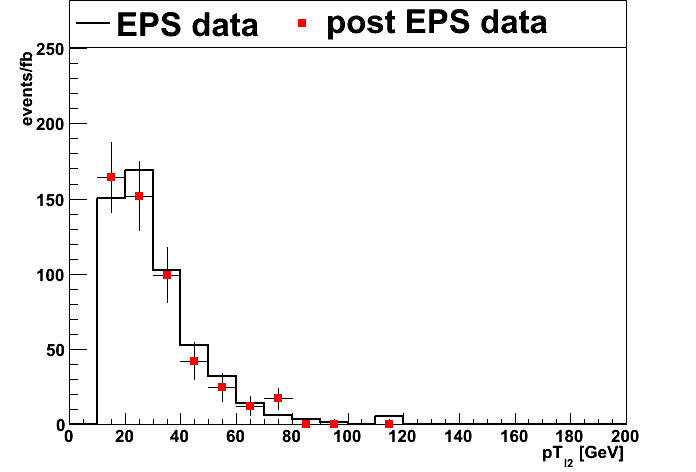
\includegraphics[width=.32\textwidth]{lp_figures/postEPSvalid/hm0/lep2pt_ww0j.png}}
\subfigure[]{
\centering
\label{subfig:lp_jet1pt_ww0j}
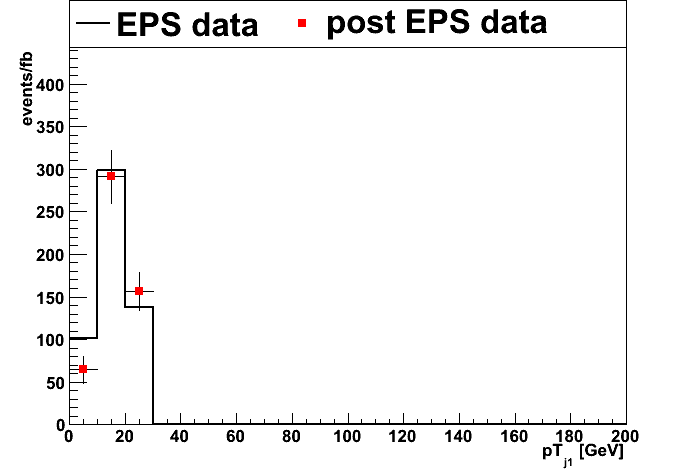
\includegraphics[width=.32\textwidth]{lp_figures/postEPSvalid/hm0/jet1pt_ww0j.png}}\\
\subfigure[]{
\centering
\label{subfig:lp_pmet_ww0j}
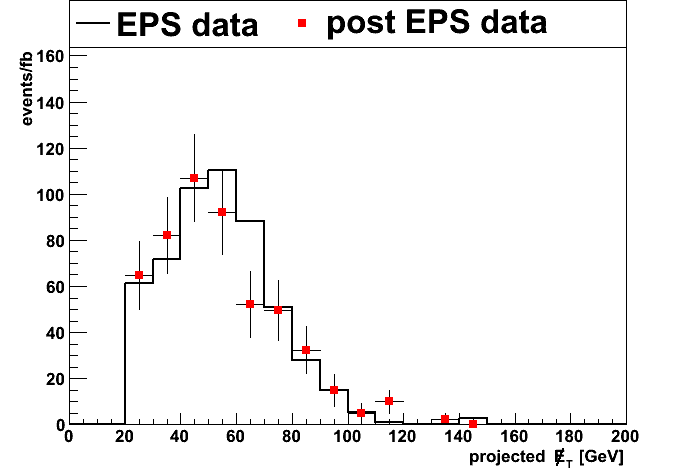
\includegraphics[width=.32\textwidth]{lp_figures/postEPSvalid/hm0/pmet_ww0j.png}}
\subfigure[]{
\centering
\label{subfig:lp_pTrackMet_ww0j}
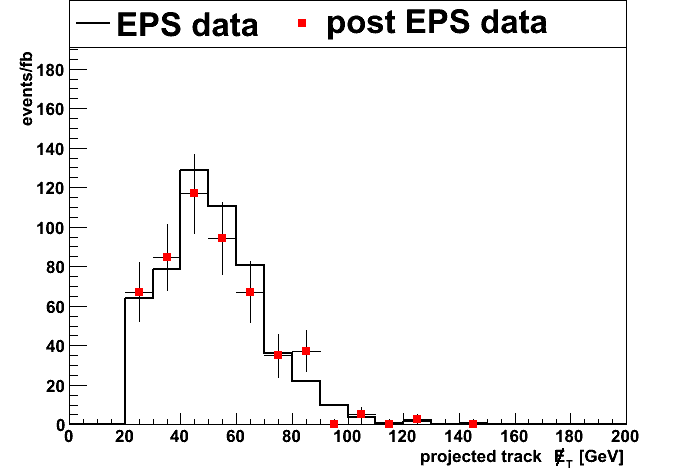
\includegraphics[width=.32\textwidth]{lp_figures/postEPSvalid/hm0/pTrackMet_ww0j.png}}
\subfigure[]{
\centering
\label{subfig:lp_mt_ww0j}
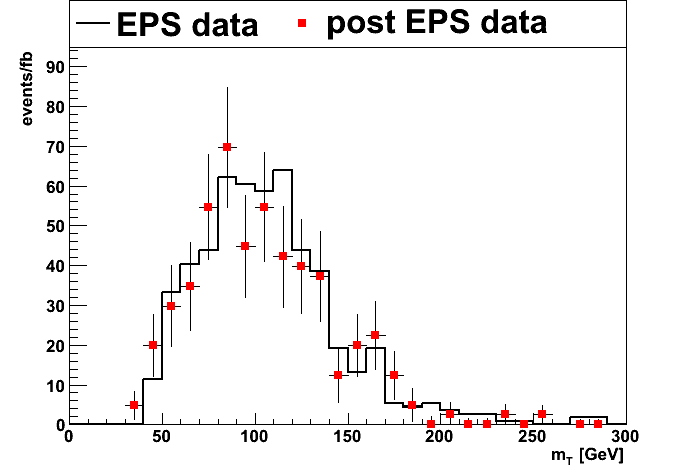
\includegraphics[width=.32\textwidth]{lp_figures/postEPSvalid/hm0/mt_ww0j.png}}
\caption{EPS and post-EPS data comparison: 0-jet bin, all final states. 
\subref{subfig:lp_lep1pt_ww0j} leading lepton $p_T$;
\subref{subfig:lp_lep2pt_ww0j} trailing lepton $p_T$;
\subref{subfig:lp_jet1pt_ww0j} leading jet $p_T$;
\subref{subfig:lp_pmet_ww0j} projected MET;
\subref{subfig:lp_pTrackMet_ww0j} projected track-MET;
\subref{subfig:lp_mt_ww0j} transverse mass of dilepton-MET system.
}
\label{fig:lp_ww0j_lepjetmet}
\end{figure}

\clearpage

\begin{figure}[!hbtp]
\centering
\subfigure[]{
\centering
\label{subfig:lp_dPhi_ww0jmm}
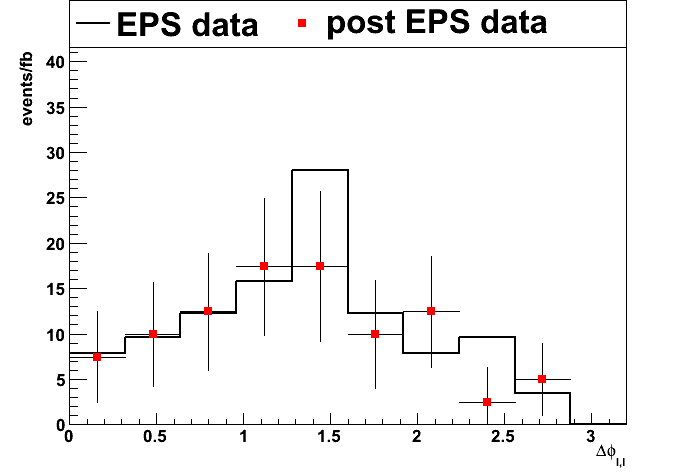
\includegraphics[width=.32\textwidth]{lp_figures/postEPSvalid/hm0/dPhi_ww0jmm.png}}
\subfigure[]{
\centering
\label{subfig:lp_dilepmass_ww0jmm}
\includegraphics[width=.32\textwidth]{lp_figures/postEPSvalid/hm0/dilepmass_ww0jmm.png}}\\
\subfigure[]{
\centering
\label{subfig:lp_dileppt_ww0jmm}
\includegraphics[width=.32\textwidth]{lp_figures/postEPSvalid/hm0/dileppt_ww0jmm.png}}
\subfigure[]{
\centering
\label{subfig:lp_type_ww0jmm}
\includegraphics[width=.32\textwidth]{lp_figures/postEPSvalid/hm0/type_ww0jmm.png}}
\caption{EPS and post-EPS data comparison: 0-jet bin, $\mu\mu$ final state. 
\subref{subfig:lp_dPhi_ww0jmm} $\Delta\phi$ between the two leptons;
\subref{subfig:lp_dilepmass_ww0jmm} di-lepton invariant mass;
\subref{subfig:lp_dileppt_ww0jmm} di-lepton transverse momentum;
\subref{subfig:lp_type_ww0jmm} di-lepton type ($\mu\mu$=0, $\mu e$=2, $e\mu$=2, $ee$=3).
}
\label{fig:lp_ww0jmm_dilep}
\end{figure}

\begin{figure}[!hbtp]
\centering
\subfigure[]{
\centering
\label{subfig:lp_lep1pt_ww0jmm}
\includegraphics[width=.32\textwidth]{lp_figures/postEPSvalid/hm0/lep1pt_ww0jmm.png}}
\subfigure[]{
\centering
\label{subfig:lp_lep2pt_ww0jmm}
\includegraphics[width=.32\textwidth]{lp_figures/postEPSvalid/hm0/lep2pt_ww0jmm.png}}
\subfigure[]{
\centering
\label{subfig:lp_jet1pt_ww0jmm}
\includegraphics[width=.32\textwidth]{lp_figures/postEPSvalid/hm0/jet1pt_ww0jmm.png}}\\
\subfigure[]{
\centering
\label{subfig:lp_pmet_ww0jmm}
\includegraphics[width=.32\textwidth]{lp_figures/postEPSvalid/hm0/pmet_ww0jmm.png}}
\subfigure[]{
\centering
\label{subfig:lp_pTrackMet_ww0jmm}
\includegraphics[width=.32\textwidth]{lp_figures/postEPSvalid/hm0/pTrackMet_ww0jmm.png}}
\subfigure[]{
\centering
\label{subfig:lp_mt_ww0jmm}
\includegraphics[width=.32\textwidth]{lp_figures/postEPSvalid/hm0/mt_ww0jmm.png}}
\caption{EPS and post-EPS data comparison: 0-jet bin, $\mu\mu$ final state. 
\subref{subfig:lp_lep1pt_ww0jmm} leading lepton $p_T$;
\subref{subfig:lp_lep2pt_ww0jmm} trailing lepton $p_T$;
\subref{subfig:lp_jet1pt_ww0jmm} leading jet $p_T$;
\subref{subfig:lp_pmet_ww0jmm} projected MET;
\subref{subfig:lp_pTrackMet_ww0jmm} projected track-MET;
\subref{subfig:lp_mt_ww0jmm} transverse mass of dilepton-MET system.
}
\label{fig:lp_ww0jmm_lepjetmet}
\end{figure}

\clearpage

\begin{figure}[!hbtp]
\centering
\subfigure[]{
\centering
\label{subfig:lp_dPhi_ww1j}
\includegraphics[width=.32\textwidth]{lp_figures/postEPSvalid/hm0/dPhi_ww1j.png}}
\subfigure[]{
\centering
\label{subfig:lp_dilepmass_ww1j}
\includegraphics[width=.32\textwidth]{lp_figures/postEPSvalid/hm0/dilepmass_ww1j.png}}\\
\subfigure[]{
\centering
\label{subfig:lp_dileppt_ww1j}
\includegraphics[width=.32\textwidth]{lp_figures/postEPSvalid/hm0/dileppt_ww1j.png}}
\subfigure[]{
\centering
\label{subfig:lp_type_ww1j}
\includegraphics[width=.32\textwidth]{lp_figures/postEPSvalid/hm0/type_ww1j.png}}
\caption{EPS and post-EPS data comparison: 1-jet bin, all final states. 
\subref{subfig:lp_dPhi_ww1j} $\Delta\phi$ between the two leptons;
\subref{subfig:lp_dilepmass_ww1j} di-lepton invariant mass;
\subref{subfig:lp_dileppt_ww1j} di-lepton transverse momentum;
\subref{subfig:lp_type_ww1j} di-lepton type ($\mu\mu$=0, $\mu e$=2, $e\mu$=2, $ee$=3).
}
\label{fig:lp_ww1j_dilep}
\end{figure}

\begin{figure}[!hbtp]
\centering
\subfigure[]{
\centering
\label{subfig:lp_lep1pt_ww1j}
\includegraphics[width=.32\textwidth]{lp_figures/postEPSvalid/hm0/lep1pt_ww1j.png}}
\subfigure[]{
\centering
\label{subfig:lp_lep2pt_ww1j}
\includegraphics[width=.32\textwidth]{lp_figures/postEPSvalid/hm0/lep2pt_ww1j.png}}
\subfigure[]{
\centering
\label{subfig:lp_jet1pt_ww1j}
\includegraphics[width=.32\textwidth]{lp_figures/postEPSvalid/hm0/jet1pt_ww1j.png}}\\
\subfigure[]{
\centering
\label{subfig:lp_pmet_ww1j}
\includegraphics[width=.32\textwidth]{lp_figures/postEPSvalid/hm0/pmet_ww1j.png}}
\subfigure[]{
\centering
\label{subfig:lp_pTrackMet_ww1j}
\includegraphics[width=.32\textwidth]{lp_figures/postEPSvalid/hm0/pTrackMet_ww1j.png}}
\subfigure[]{
\centering
\label{subfig:lp_mt_ww1j}
\includegraphics[width=.32\textwidth]{lp_figures/postEPSvalid/hm0/mt_ww1j.png}}
\caption{EPS and post-EPS data comparison: 1-jet bin, all final states. 
\subref{subfig:lp_lep1pt_ww1j} leading lepton $p_T$;
\subref{subfig:lp_lep2pt_ww1j} trailing lepton $p_T$;
\subref{subfig:lp_jet1pt_ww1j} leading jet $p_T$;
\subref{subfig:lp_pmet_ww1j} projected MET;
\subref{subfig:lp_pTrackMet_ww1j} projected track-MET;
\subref{subfig:lp_mt_ww1j} transverse mass of dilepton-MET system.
}
\label{fig:lp_ww1j_lepjetmet}
\end{figure}

\clearpage

\begin{figure}[!hbtp]
\centering
\subfigure[]{
\centering
\label{subfig:lp_dPhi_ww2j}
\includegraphics[width=.32\textwidth]{lp_figures/postEPSvalid/hm0/dPhi_ww2j.png}}
\subfigure[]{
\centering
\label{subfig:lp_dilepmass_ww2j}
\includegraphics[width=.32\textwidth]{lp_figures/postEPSvalid/hm0/dilepmass_ww2j.png}}\\
\subfigure[]{
\centering
\label{subfig:lp_dileppt_ww2j}
\includegraphics[width=.32\textwidth]{lp_figures/postEPSvalid/hm0/dileppt_ww2j.png}}
\subfigure[]{
\centering
\label{subfig:lp_type_ww2j}
\includegraphics[width=.32\textwidth]{lp_figures/postEPSvalid/hm0/type_ww2j.png}}
\caption{EPS and post-EPS data comparison: 2-jet bin, all final states. 
\subref{subfig:lp_dPhi_ww2j} $\Delta\phi$ between the two leptons;
\subref{subfig:lp_dilepmass_ww2j} di-lepton invariant mass;
\subref{subfig:lp_dileppt_ww2j} di-lepton transverse momentum;
\subref{subfig:lp_type_ww2j} di-lepton type ($\mu\mu$=0, $\mu e$=2, $e\mu$=2, $ee$=3).
}
\label{fig:lp_ww2j_dilep}
\end{figure}

\begin{figure}[!hbtp]
\centering
\subfigure[]{
\centering
\label{subfig:lp_lep1pt_ww2j}
\includegraphics[width=.32\textwidth]{lp_figures/postEPSvalid/hm0/lep1pt_ww2j.png}}
\subfigure[]{
\centering
\label{subfig:lp_lep2pt_ww2j}
\includegraphics[width=.32\textwidth]{lp_figures/postEPSvalid/hm0/lep2pt_ww2j.png}}
\subfigure[]{
\centering
\label{subfig:lp_jet1pt_ww2j}
\includegraphics[width=.32\textwidth]{lp_figures/postEPSvalid/hm0/jet1pt_ww2j.png}}\\
\subfigure[]{
\centering
\label{subfig:lp_pmet_ww2j}
\includegraphics[width=.32\textwidth]{lp_figures/postEPSvalid/hm0/pmet_ww2j.png}}
\subfigure[]{
\centering
\label{subfig:lp_pTrackMet_ww2j}
\includegraphics[width=.32\textwidth]{lp_figures/postEPSvalid/hm0/pTrackMet_ww2j.png}}
\subfigure[]{
\centering
\label{subfig:lp_mt_ww2j}
\includegraphics[width=.32\textwidth]{lp_figures/postEPSvalid/hm0/mt_ww2j.png}}
\caption{EPS and post-EPS data comparison: 2-jet bin, all final states. 
\subref{subfig:lp_lep1pt_ww2j} leading lepton $p_T$;
\subref{subfig:lp_lep2pt_ww2j} trailing lepton $p_T$;
\subref{subfig:lp_jet1pt_ww2j} leading jet $p_T$;
\subref{subfig:lp_pmet_ww2j} projected MET;
\subref{subfig:lp_pTrackMet_ww2j} projected track-MET;
\subref{subfig:lp_mt_ww2j} transverse mass of dilepton-MET system.
}
\label{fig:lp_ww2j_lepjetmet}
\end{figure}

\clearpage


%%      \subsubsection{Lepton and Trigger Efficiency}
%%      This is a Lepton and Trigger Efficiency

%%      \subsubsection{PU reweighting}
%%      This is a PU reweighting

%%     \subsubsection{Summary of Data Validation}
%%     
We find the post-EPS data to be consistent with the EPS data with regard to trigger and
lepton efficiencies. We find good agreement between data and MC for the distribution of the number
of reconstructed vertices per event after re-weighting based on the expected number of pile-up events.
We inspected the relevant kinematic variables (see Section \ref{app:lp_postEPSdist} for details) and find no significant
discrepancies between the two data samples.



%%      \subsection{Background Estimation for \lpintlumi}
%%     \label{app:lp_bkgestim}
%%      This is a background Estimation for 1.545$\fb$


%%      \subsection{Final limits for \lpintlumi}
%%     \label{app:lp_limits}
%%      This is a final limit


%%      \subsection{Conclusions}
%%      This is a conclusion



%%     \subsection{MVA output plots}
%%     \label{app:lp_mvaplots}
%%     \subsubsection{EPS distributions}

This section contains the MVA output plots for the EPS dataset for $m_H$=115, 120, 130, 140, 150, 160, 200 GeV analyses split in opposte and same flavor, 
0-jet and 1-jet bin (Figures~\ref{fig:lp_mva_115_EPS}-\ref{fig:lp_mva_200_EPS}).

\begin{figure}[!hbtp]
\centering
\subfigure[]{
\centering
\label{subfig:lp_mva_115_0j_of_EPS}
\includegraphics[width=.40\textwidth]{lp_figures/histo_mva_115_0j_of_EPS.png}}
\subfigure[]{
\centering
\label{subfig:lp_mva_115_0j_sf_EPS}
\includegraphics[width=.40\textwidth]{lp_figures/histo_mva_115_0j_sf_EPS.png}}\\
\subfigure[]{
\centering
\label{subfig:lp_mva_115_1j_of_EPS}
\includegraphics[width=.40\textwidth]{lp_figures/histo_mva_115_1j_of_EPS.png}}
\subfigure[]{
\centering
\label{subfig:lp_mva_115_1j_sf_EPS}
\includegraphics[width=.40\textwidth]{lp_figures/histo_mva_115_1j_sf_EPS.png}}
\caption{
MVA output for $m_H$=115 GeV EPS analysis: 
0-jet OF \subref{subfig:lp_mva_115_0j_of_EPS},
0-jet SF \subref{subfig:lp_mva_115_0j_sf_EPS},
1-jet OF \subref{subfig:lp_mva_115_1j_of_EPS},
1-jet SF \subref{subfig:lp_mva_115_1j_sf_EPS}
.}
\label{fig:lp_mva_115_EPS}
\end{figure}

\begin{figure}[!hbtp]
\centering
\subfigure[]{
\centering
\label{subfig:lp_mva_120_0j_of_EPS}
\includegraphics[width=.40\textwidth]{lp_figures/histo_mva_120_0j_of_EPS.png}}
\subfigure[]{
\centering
\label{subfig:lp_mva_120_0j_sf_EPS}
\includegraphics[width=.40\textwidth]{lp_figures/histo_mva_120_0j_sf_EPS.png}}\\
\subfigure[]{
\centering
\label{subfig:lp_mva_120_1j_of_EPS}
\includegraphics[width=.40\textwidth]{lp_figures/histo_mva_120_1j_of_EPS.png}}
\subfigure[]{
\centering
\label{subfig:lp_mva_120_1j_sf_EPS}
\includegraphics[width=.40\textwidth]{lp_figures/histo_mva_120_1j_sf_EPS.png}}
\caption{
MVA output for $m_H$=120 GeV EPS analysis: 
0-jet OF \subref{subfig:lp_mva_120_0j_of_EPS},
0-jet SF \subref{subfig:lp_mva_120_0j_sf_EPS},
1-jet OF \subref{subfig:lp_mva_120_1j_of_EPS},
1-jet SF \subref{subfig:lp_mva_120_1j_sf_EPS}
.}
\label{fig:lp_mva_120_EPS}
\end{figure}

\begin{figure}[!hbtp]
\centering
\subfigure[]{
\centering
\label{subfig:lp_mva_130_0j_of_EPS}
\includegraphics[width=.40\textwidth]{lp_figures/histo_mva_130_0j_of_EPS.png}}
\subfigure[]{
\centering
\label{subfig:lp_mva_130_0j_sf_EPS}
\includegraphics[width=.40\textwidth]{lp_figures/histo_mva_130_0j_sf_EPS.png}}\\
\subfigure[]{
\centering
\label{subfig:lp_mva_130_1j_of_EPS}
\includegraphics[width=.40\textwidth]{lp_figures/histo_mva_130_1j_of_EPS.png}}
\subfigure[]{
\centering
\label{subfig:lp_mva_130_1j_sf_EPS}
\includegraphics[width=.40\textwidth]{lp_figures/histo_mva_130_1j_sf_EPS.png}}
\caption{
MVA output for $m_H$=130 GeV EPS analysis: 
0-jet OF \subref{subfig:lp_mva_130_0j_of_EPS},
0-jet SF \subref{subfig:lp_mva_130_0j_sf_EPS},
1-jet OF \subref{subfig:lp_mva_130_1j_of_EPS},
1-jet SF \subref{subfig:lp_mva_130_1j_sf_EPS}
.}
\label{fig:lp_mva_130_EPS}
\end{figure}

\begin{figure}[!hbtp]
\centering
\subfigure[]{
\centering
\label{subfig:lp_mva_140_0j_of_EPS}
\includegraphics[width=.40\textwidth]{lp_figures/histo_mva_140_0j_of_EPS.png}}
\subfigure[]{
\centering
\label{subfig:lp_mva_140_0j_sf_EPS}
\includegraphics[width=.40\textwidth]{lp_figures/histo_mva_140_0j_sf_EPS.png}}\\
\subfigure[]{
\centering
\label{subfig:lp_mva_140_1j_of_EPS}
\includegraphics[width=.40\textwidth]{lp_figures/histo_mva_140_1j_of_EPS.png}}
\subfigure[]{
\centering
\label{subfig:lp_mva_140_1j_sf_EPS}
\includegraphics[width=.40\textwidth]{lp_figures/histo_mva_140_1j_sf_EPS.png}}
\caption{
MVA output for $m_H$=140 GeV EPS analysis: 
0-jet OF \subref{subfig:lp_mva_140_0j_of_EPS},
0-jet SF \subref{subfig:lp_mva_140_0j_sf_EPS},
1-jet OF \subref{subfig:lp_mva_140_1j_of_EPS},
1-jet SF \subref{subfig:lp_mva_140_1j_sf_EPS}
.}
\label{fig:lp_mva_140_EPS}
\end{figure}

\begin{figure}[!hbtp]
\centering
\subfigure[]{
\centering
\label{subfig:lp_mva_150_0j_of_EPS}
\includegraphics[width=.40\textwidth]{lp_figures/histo_mva_150_0j_of_EPS.png}}
\subfigure[]{
\centering
\label{subfig:lp_mva_150_0j_sf_EPS}
\includegraphics[width=.40\textwidth]{lp_figures/histo_mva_150_0j_sf_EPS.png}}\\
\subfigure[]{
\centering
\label{subfig:lp_mva_150_1j_of_EPS}
\includegraphics[width=.40\textwidth]{lp_figures/histo_mva_150_1j_of_EPS.png}}
\subfigure[]{
\centering
\label{subfig:lp_mva_150_1j_sf_EPS}
\includegraphics[width=.40\textwidth]{lp_figures/histo_mva_150_1j_sf_EPS.png}}
\caption{
MVA output for $m_H$=150 GeV EPS analysis: 
0-jet OF \subref{subfig:lp_mva_150_0j_of_EPS},
0-jet SF \subref{subfig:lp_mva_150_0j_sf_EPS},
1-jet OF \subref{subfig:lp_mva_150_1j_of_EPS},
1-jet SF \subref{subfig:lp_mva_150_1j_sf_EPS}
.}
\label{fig:lp_mva_150_EPS}
\end{figure}

\begin{figure}[!hbtp]
\centering
\subfigure[]{
\centering
\label{subfig:lp_mva_160_0j_of_EPS}
\includegraphics[width=.40\textwidth]{lp_figures/histo_mva_160_0j_of_EPS.png}}
\subfigure[]{
\centering
\label{subfig:lp_mva_160_0j_sf_EPS}
\includegraphics[width=.40\textwidth]{lp_figures/histo_mva_160_0j_sf_EPS.png}}\\
\subfigure[]{
\centering
\label{subfig:lp_mva_160_1j_of_EPS}
\includegraphics[width=.40\textwidth]{lp_figures/histo_mva_160_1j_of_EPS.png}}
\subfigure[]{
\centering
\label{subfig:lp_mva_160_1j_sf_EPS}
\includegraphics[width=.40\textwidth]{lp_figures/histo_mva_160_1j_sf_EPS.png}}
\caption{
MVA output for $m_H$=160 GeV EPS analysis: 
0-jet OF \subref{subfig:lp_mva_160_0j_of_EPS},
0-jet SF \subref{subfig:lp_mva_160_0j_sf_EPS},
1-jet OF \subref{subfig:lp_mva_160_1j_of_EPS},
1-jet SF \subref{subfig:lp_mva_160_1j_sf_EPS}
.}
\label{fig:lp_mva_160_EPS}
\end{figure}

\begin{figure}[!hbtp]
\centering
\subfigure[]{
\centering
\label{subfig:lp_mva_200_0j_of_EPS}
\includegraphics[width=.40\textwidth]{lp_figures/histo_mva_200_0j_of_EPS.png}}
\subfigure[]{
\centering
\label{subfig:lp_mva_200_0j_sf_EPS}
\includegraphics[width=.40\textwidth]{lp_figures/histo_mva_200_0j_sf_EPS.png}}\\
\subfigure[]{
\centering
\label{subfig:lp_mva_200_1j_of_EPS}
\includegraphics[width=.40\textwidth]{lp_figures/histo_mva_200_1j_of_EPS.png}}
\subfigure[]{
\centering
\label{subfig:lp_mva_200_1j_sf_EPS}
\includegraphics[width=.40\textwidth]{lp_figures/histo_mva_200_1j_sf_EPS.png}}
\caption{
MVA output for $m_H$=200 GeV EPS analysis: 
0-jet OF \subref{subfig:lp_mva_200_0j_of_EPS},
0-jet SF \subref{subfig:lp_mva_200_0j_sf_EPS},
1-jet OF \subref{subfig:lp_mva_200_1j_of_EPS},
1-jet SF \subref{subfig:lp_mva_200_1j_sf_EPS}
.}
\label{fig:lp_mva_200_EPS}
\end{figure}

\clearpage

%%     \subsection{Post-EPS distributions}

This section contains the MVA output plots for the post-EPS dataset for $m_H$=115, 120, 130, 140, 150, 160, 200 GeV analyses split in opposte and same flavor, 
0-jet and 1-jet bin (Figures~\ref{fig:lp_mva_115_POSTEPS}-\ref{fig:lp_mva_200_POSTEPS}).

\begin{figure}[!hbtp]
\centering
\subfigure[]{
\centering
\label{subfig:lp_mva_115_0j_of_POSTEPS}
\includegraphics[width=.40\textwidth]{lp_figures/histo_mva_115_0j_of_POSTEPS.png}}
\subfigure[]{
\centering
\label{subfig:lp_mva_115_0j_sf_POSTEPS}
\includegraphics[width=.40\textwidth]{lp_figures/histo_mva_115_0j_sf_POSTEPS.png}}\\
\subfigure[]{
\centering
\label{subfig:lp_mva_115_1j_of_POSTEPS}
\includegraphics[width=.40\textwidth]{lp_figures/histo_mva_115_1j_of_POSTEPS.png}}
\subfigure[]{
\centering
\label{subfig:lp_mva_115_1j_sf_POSTEPS}
\includegraphics[width=.40\textwidth]{lp_figures/histo_mva_115_1j_sf_POSTEPS.png}}
\caption{
MVA output for $m_H$=115 GeV post-EPS analysis: 
0-jet OF \subref{subfig:lp_mva_115_0j_of_POSTEPS},
0-jet SF \subref{subfig:lp_mva_115_0j_sf_POSTEPS},
1-jet OF \subref{subfig:lp_mva_115_1j_of_POSTEPS},
1-jet SF \subref{subfig:lp_mva_115_1j_sf_POSTEPS}
.}
\label{fig:lp_mva_115_POSTEPS}
\end{figure}

\begin{figure}[!hbtp]
\centering
\subfigure[]{
\centering
\label{subfig:lp_mva_120_0j_of_POSTEPS}
\includegraphics[width=.40\textwidth]{lp_figures/histo_mva_120_0j_of_POSTEPS.png}}
\subfigure[]{
\centering
\label{subfig:lp_mva_120_0j_sf_POSTEPS}
\includegraphics[width=.40\textwidth]{lp_figures/histo_mva_120_0j_sf_POSTEPS.png}}\\
\subfigure[]{
\centering
\label{subfig:lp_mva_120_1j_of_POSTEPS}
\includegraphics[width=.40\textwidth]{lp_figures/histo_mva_120_1j_of_POSTEPS.png}}
\subfigure[]{
\centering
\label{subfig:lp_mva_120_1j_sf_POSTEPS}
\includegraphics[width=.40\textwidth]{lp_figures/histo_mva_120_1j_sf_POSTEPS.png}}
\caption{
MVA output for $m_H$=120 GeV post-EPS analysis: 
0-jet OF \subref{subfig:lp_mva_120_0j_of_POSTEPS},
0-jet SF \subref{subfig:lp_mva_120_0j_sf_POSTEPS},
1-jet OF \subref{subfig:lp_mva_120_1j_of_POSTEPS},
1-jet SF \subref{subfig:lp_mva_120_1j_sf_POSTEPS}
.}
\label{fig:lp_mva_120_POSTEPS}
\end{figure}

\begin{figure}[!hbtp]
\centering
\subfigure[]{
\centering
\label{subfig:lp_mva_130_0j_of_POSTEPS}
\includegraphics[width=.40\textwidth]{lp_figures/histo_mva_130_0j_of_POSTEPS.png}}
\subfigure[]{
\centering
\label{subfig:lp_mva_130_0j_sf_POSTEPS}
\includegraphics[width=.40\textwidth]{lp_figures/histo_mva_130_0j_sf_POSTEPS.png}}\\
\subfigure[]{
\centering
\label{subfig:lp_mva_130_1j_of_POSTEPS}
\includegraphics[width=.40\textwidth]{lp_figures/histo_mva_130_1j_of_POSTEPS.png}}
\subfigure[]{
\centering
\label{subfig:lp_mva_130_1j_sf_POSTEPS}
\includegraphics[width=.40\textwidth]{lp_figures/histo_mva_130_1j_sf_POSTEPS.png}}
\caption{
MVA output for $m_H$=130 GeV post-EPS analysis: 
0-jet OF \subref{subfig:lp_mva_130_0j_of_POSTEPS},
0-jet SF \subref{subfig:lp_mva_130_0j_sf_POSTEPS},
1-jet OF \subref{subfig:lp_mva_130_1j_of_POSTEPS},
1-jet SF \subref{subfig:lp_mva_130_1j_sf_POSTEPS}
.}
\label{fig:lp_mva_130_POSTEPS}
\end{figure}

\begin{figure}[!hbtp]
\centering
\subfigure[]{
\centering
\label{subfig:lp_mva_140_0j_of_POSTEPS}
\includegraphics[width=.40\textwidth]{lp_figures/histo_mva_140_0j_of_POSTEPS.png}}
\subfigure[]{
\centering
\label{subfig:lp_mva_140_0j_sf_POSTEPS}
\includegraphics[width=.40\textwidth]{lp_figures/histo_mva_140_0j_sf_POSTEPS.png}}\\
\subfigure[]{
\centering
\label{subfig:lp_mva_140_1j_of_POSTEPS}
\includegraphics[width=.40\textwidth]{lp_figures/histo_mva_140_1j_of_POSTEPS.png}}
\subfigure[]{
\centering
\label{subfig:lp_mva_140_1j_sf_POSTEPS}
\includegraphics[width=.40\textwidth]{lp_figures/histo_mva_140_1j_sf_POSTEPS.png}}
\caption{
MVA output for $m_H$=140 GeV post-EPS analysis: 
0-jet OF \subref{subfig:lp_mva_140_0j_of_POSTEPS},
0-jet SF \subref{subfig:lp_mva_140_0j_sf_POSTEPS},
1-jet OF \subref{subfig:lp_mva_140_1j_of_POSTEPS},
1-jet SF \subref{subfig:lp_mva_140_1j_sf_POSTEPS}
.}
\label{fig:lp_mva_140_POSTEPS}
\end{figure}

\begin{figure}[!hbtp]
\centering
\subfigure[]{
\centering
\label{subfig:lp_mva_150_0j_of_POSTEPS}
\includegraphics[width=.40\textwidth]{lp_figures/histo_mva_150_0j_of_POSTEPS.png}}
\subfigure[]{
\centering
\label{subfig:lp_mva_150_0j_sf_POSTEPS}
\includegraphics[width=.40\textwidth]{lp_figures/histo_mva_150_0j_sf_POSTEPS.png}}\\
\subfigure[]{
\centering
\label{subfig:lp_mva_150_1j_of_POSTEPS}
\includegraphics[width=.40\textwidth]{lp_figures/histo_mva_150_1j_of_POSTEPS.png}}
\subfigure[]{
\centering
\label{subfig:lp_mva_150_1j_sf_POSTEPS}
\includegraphics[width=.40\textwidth]{lp_figures/histo_mva_150_1j_sf_POSTEPS.png}}
\caption{
MVA output for $m_H$=150 GeV post-EPS analysis: 
0-jet OF \subref{subfig:lp_mva_150_0j_of_POSTEPS},
0-jet SF \subref{subfig:lp_mva_150_0j_sf_POSTEPS},
1-jet OF \subref{subfig:lp_mva_150_1j_of_POSTEPS},
1-jet SF \subref{subfig:lp_mva_150_1j_sf_POSTEPS}
.}
\label{fig:lp_mva_150_POSTEPS}
\end{figure}

\begin{figure}[!hbtp]
\centering
\subfigure[]{
\centering
\label{subfig:lp_mva_160_0j_of_POSTEPS}
\includegraphics[width=.40\textwidth]{lp_figures/histo_mva_160_0j_of_POSTEPS.png}}
\subfigure[]{
\centering
\label{subfig:lp_mva_160_0j_sf_POSTEPS}
\includegraphics[width=.40\textwidth]{lp_figures/histo_mva_160_0j_sf_POSTEPS.png}}\\
\subfigure[]{
\centering
\label{subfig:lp_mva_160_1j_of_POSTEPS}
\includegraphics[width=.40\textwidth]{lp_figures/histo_mva_160_1j_of_POSTEPS.png}}
\subfigure[]{
\centering
\label{subfig:lp_mva_160_1j_sf_POSTEPS}
\includegraphics[width=.40\textwidth]{lp_figures/histo_mva_160_1j_sf_POSTEPS.png}}
\caption{
MVA output for $m_H$=160 GeV post-EPS analysis: 
0-jet OF \subref{subfig:lp_mva_160_0j_of_POSTEPS},
0-jet SF \subref{subfig:lp_mva_160_0j_sf_POSTEPS},
1-jet OF \subref{subfig:lp_mva_160_1j_of_POSTEPS},
1-jet SF \subref{subfig:lp_mva_160_1j_sf_POSTEPS}
.}
\label{fig:lp_mva_160_POSTEPS}
\end{figure}

\begin{figure}[!hbtp]
\centering
\subfigure[]{
\centering
\label{subfig:lp_mva_200_0j_of_POSTEPS}
\includegraphics[width=.40\textwidth]{lp_figures/histo_mva_200_0j_of_POSTEPS.png}}
\subfigure[]{
\centering
\label{subfig:lp_mva_200_0j_sf_POSTEPS}
\includegraphics[width=.40\textwidth]{lp_figures/histo_mva_200_0j_sf_POSTEPS.png}}\\
\subfigure[]{
\centering
\label{subfig:lp_mva_200_1j_of_POSTEPS}
\includegraphics[width=.40\textwidth]{lp_figures/histo_mva_200_1j_of_POSTEPS.png}}
\subfigure[]{
\centering
\label{subfig:lp_mva_200_1j_sf_POSTEPS}
\includegraphics[width=.40\textwidth]{lp_figures/histo_mva_200_1j_sf_POSTEPS.png}}
\caption{
MVA output for $m_H$=200 GeV post-EPS analysis: 
0-jet OF \subref{subfig:lp_mva_200_0j_of_POSTEPS},
0-jet SF \subref{subfig:lp_mva_200_0j_sf_POSTEPS},
1-jet OF \subref{subfig:lp_mva_200_1j_of_POSTEPS},
1-jet SF \subref{subfig:lp_mva_200_1j_sf_POSTEPS}
.}
\label{fig:lp_mva_200_POSTEPS}
\end{figure}

\clearpage

%%     \subsection{LP distributions}

This section contains the MVA output plots for the LP dataset for $m_H$=115, 120, 130, 140, 150, 160, 200 GeV analyses split in opposte and same flavor, 
0-jet and 1-jet bin (Figures~\ref{fig:lp_mva_115}-\ref{fig:lp_mva_200}).

\begin{figure}[!hbtp]
\centering
\subfigure[]{
\centering
\label{subfig:lp_mva_115_0j_of}
\includegraphics[width=.40\textwidth]{lp_figures/histo_mva_115_0j_of.png}}
\subfigure[]{
\centering
\label{subfig:lp_mva_115_0j_sf}
\includegraphics[width=.40\textwidth]{lp_figures/histo_mva_115_0j_sf.png}}\\
\subfigure[]{
\centering
\label{subfig:lp_mva_115_1j_of}
\includegraphics[width=.40\textwidth]{lp_figures/histo_mva_115_1j_of.png}}
\subfigure[]{
\centering
\label{subfig:lp_mva_115_1j_sf}
\includegraphics[width=.40\textwidth]{lp_figures/histo_mva_115_1j_sf.png}}
\caption{
MVA output for $m_H$=115 GeV LP analysis: 
0-jet OF \subref{subfig:lp_mva_115_0j_of},
0-jet SF \subref{subfig:lp_mva_115_0j_sf},
1-jet OF \subref{subfig:lp_mva_115_1j_of},
1-jet SF \subref{subfig:lp_mva_115_1j_sf}
.}
\label{fig:lp_mva_115}
\end{figure}

\begin{figure}[!hbtp]
\centering
\subfigure[]{
\centering
\label{subfig:lp_mva_120_0j_of}
\includegraphics[width=.40\textwidth]{lp_figures/histo_mva_120_0j_of.png}}
\subfigure[]{
\centering
\label{subfig:lp_mva_120_0j_sf}
\includegraphics[width=.40\textwidth]{lp_figures/histo_mva_120_0j_sf.png}}\\
\subfigure[]{
\centering
\label{subfig:lp_mva_120_1j_of}
\includegraphics[width=.40\textwidth]{lp_figures/histo_mva_120_1j_of.png}}
\subfigure[]{
\centering
\label{subfig:lp_mva_120_1j_sf}
\includegraphics[width=.40\textwidth]{lp_figures/histo_mva_120_1j_sf.png}}
\caption{
MVA output for $m_H$=120 GeV LP analysis: 
0-jet OF \subref{subfig:lp_mva_120_0j_of},
0-jet SF \subref{subfig:lp_mva_120_0j_sf},
1-jet OF \subref{subfig:lp_mva_120_1j_of},
1-jet SF \subref{subfig:lp_mva_120_1j_sf}
.}
\label{fig:lp_mva_120}
\end{figure}

\begin{figure}[!hbtp]
\centering
\subfigure[]{
\centering
\label{subfig:lp_mva_130_0j_of}
\includegraphics[width=.40\textwidth]{lp_figures/histo_mva_130_0j_of.png}}
\subfigure[]{
\centering
\label{subfig:lp_mva_130_0j_sf}
\includegraphics[width=.40\textwidth]{lp_figures/histo_mva_130_0j_sf.png}}\\
\subfigure[]{
\centering
\label{subfig:lp_mva_130_1j_of}
\includegraphics[width=.40\textwidth]{lp_figures/histo_mva_130_1j_of.png}}
\subfigure[]{
\centering
\label{subfig:lp_mva_130_1j_sf}
\includegraphics[width=.40\textwidth]{lp_figures/histo_mva_130_1j_sf.png}}
\caption{
MVA output for $m_H$=130 GeV LP analysis: 
0-jet OF \subref{subfig:lp_mva_130_0j_of},
0-jet SF \subref{subfig:lp_mva_130_0j_sf},
1-jet OF \subref{subfig:lp_mva_130_1j_of},
1-jet SF \subref{subfig:lp_mva_130_1j_sf}
.}
\label{fig:lp_mva_130}
\end{figure}

\begin{figure}[!hbtp]
\centering
\subfigure[]{
\centering
\label{subfig:lp_mva_140_0j_of}
\includegraphics[width=.40\textwidth]{lp_figures/histo_mva_140_0j_of.png}}
\subfigure[]{
\centering
\label{subfig:lp_mva_140_0j_sf}
\includegraphics[width=.40\textwidth]{lp_figures/histo_mva_140_0j_sf.png}}\\
\subfigure[]{
\centering
\label{subfig:lp_mva_140_1j_of}
\includegraphics[width=.40\textwidth]{lp_figures/histo_mva_140_1j_of.png}}
\subfigure[]{
\centering
\label{subfig:lp_mva_140_1j_sf}
\includegraphics[width=.40\textwidth]{lp_figures/histo_mva_140_1j_sf.png}}
\caption{
MVA output for $m_H$=140 GeV LP analysis: 
0-jet OF \subref{subfig:lp_mva_140_0j_of},
0-jet SF \subref{subfig:lp_mva_140_0j_sf},
1-jet OF \subref{subfig:lp_mva_140_1j_of},
1-jet SF \subref{subfig:lp_mva_140_1j_sf}
.}
\label{fig:lp_mva_140}
\end{figure}

\begin{figure}[!hbtp]
\centering
\subfigure[]{
\centering
\label{subfig:lp_mva_150_0j_of}
\includegraphics[width=.40\textwidth]{lp_figures/histo_mva_150_0j_of.png}}
\subfigure[]{
\centering
\label{subfig:lp_mva_150_0j_sf}
\includegraphics[width=.40\textwidth]{lp_figures/histo_mva_150_0j_sf.png}}\\
\subfigure[]{
\centering
\label{subfig:lp_mva_150_1j_of}
\includegraphics[width=.40\textwidth]{lp_figures/histo_mva_150_1j_of.png}}
\subfigure[]{
\centering
\label{subfig:lp_mva_150_1j_sf}
\includegraphics[width=.40\textwidth]{lp_figures/histo_mva_150_1j_sf.png}}
\caption{
MVA output for $m_H$=150 GeV LP analysis: 
0-jet OF \subref{subfig:lp_mva_150_0j_of},
0-jet SF \subref{subfig:lp_mva_150_0j_sf},
1-jet OF \subref{subfig:lp_mva_150_1j_of},
1-jet SF \subref{subfig:lp_mva_150_1j_sf}
.}
\label{fig:lp_mva_150}
\end{figure}

\begin{figure}[!hbtp]
\centering
\subfigure[]{
\centering
\label{subfig:lp_mva_160_0j_of}
\includegraphics[width=.40\textwidth]{lp_figures/histo_mva_160_0j_of.png}}
\subfigure[]{
\centering
\label{subfig:lp_mva_160_0j_sf}
\includegraphics[width=.40\textwidth]{lp_figures/histo_mva_160_0j_sf.png}}\\
\subfigure[]{
\centering
\label{subfig:lp_mva_160_1j_of}
\includegraphics[width=.40\textwidth]{lp_figures/histo_mva_160_1j_of.png}}
\subfigure[]{
\centering
\label{subfig:lp_mva_160_1j_sf}
\includegraphics[width=.40\textwidth]{lp_figures/histo_mva_160_1j_sf.png}}
\caption{
MVA output for $m_H$=160 GeV LP analysis: 
0-jet OF \subref{subfig:lp_mva_160_0j_of},
0-jet SF \subref{subfig:lp_mva_160_0j_sf},
1-jet OF \subref{subfig:lp_mva_160_1j_of},
1-jet SF \subref{subfig:lp_mva_160_1j_sf}
.}
\label{fig:lp_mva_160}
\end{figure}

\begin{figure}[!hbtp]
\centering
\subfigure[]{
\centering
\label{subfig:lp_mva_200_0j_of}
\includegraphics[width=.40\textwidth]{lp_figures/histo_mva_200_0j_of.png}}
\subfigure[]{
\centering
\label{subfig:lp_mva_200_0j_sf}
\includegraphics[width=.40\textwidth]{lp_figures/histo_mva_200_0j_sf.png}}\\
\subfigure[]{
\centering
\label{subfig:lp_mva_200_1j_of}
\includegraphics[width=.40\textwidth]{lp_figures/histo_mva_200_1j_of.png}}
\subfigure[]{
\centering
\label{subfig:lp_mva_200_1j_sf}
\includegraphics[width=.40\textwidth]{lp_figures/histo_mva_200_1j_sf.png}}
\caption{
MVA output for $m_H$=200 GeV LP analysis: 
0-jet OF \subref{subfig:lp_mva_200_0j_of},
0-jet SF \subref{subfig:lp_mva_200_0j_sf},
1-jet OF \subref{subfig:lp_mva_200_1j_of},
1-jet SF \subref{subfig:lp_mva_200_1j_sf}
.}
\label{fig:lp_mva_200}
\end{figure}

\clearpage

%%     \subsubsection{LP distributions with $80<m_T<m_H$}

This section contains the MVA output plots for the LP dataset for $m_H$=115, 120, 130, 140, 150, 160, 200 GeV analyses split in opposte and same flavor, 
0-jet and 1-jet bin requiring a transverse mass value greater than 80 GeV and smaller than the considered Higgs mass 
(Figures~\ref{fig:lp_mva_115_MTCUTGT80}-\ref{fig:lp_mva_200_MTCUTGT80}).

\begin{figure}[!hbtp]
\centering
\subfigure[]{
\centering
\label{subfig:lp_mva_115_0j_of_MTCUTGT80}
\includegraphics[width=.40\textwidth]{lp_figures/histo_mva_115_0j_of_MTCUTGT80.png}}
\subfigure[]{
\centering
\label{subfig:lp_mva_115_0j_sf_MTCUTGT80}
\includegraphics[width=.40\textwidth]{lp_figures/histo_mva_115_0j_sf_MTCUTGT80.png}}\\
\subfigure[]{
\centering
\label{subfig:lp_mva_115_1j_of_MTCUTGT80}
\includegraphics[width=.40\textwidth]{lp_figures/histo_mva_115_1j_of_MTCUTGT80.png}}
\subfigure[]{
\centering
\label{subfig:lp_mva_115_1j_sf_MTCUTGT80}
\includegraphics[width=.40\textwidth]{lp_figures/histo_mva_115_1j_sf_MTCUTGT80.png}}
\caption{
MVA output for $m_H$=115 GeV LP ($80<m_T<m_H$) analysis: 
0-jet OF \subref{subfig:lp_mva_115_0j_of_MTCUTGT80},
0-jet SF \subref{subfig:lp_mva_115_0j_sf_MTCUTGT80},
1-jet OF \subref{subfig:lp_mva_115_1j_of_MTCUTGT80},
1-jet SF \subref{subfig:lp_mva_115_1j_sf_MTCUTGT80}
.}
\label{fig:lp_mva_115_MTCUTGT80}
\end{figure}

\begin{figure}[!hbtp]
\centering
\subfigure[]{
\centering
\label{subfig:lp_mva_120_0j_of_MTCUTGT80}
\includegraphics[width=.40\textwidth]{lp_figures/histo_mva_120_0j_of_MTCUTGT80.png}}
\subfigure[]{
\centering
\label{subfig:lp_mva_120_0j_sf_MTCUTGT80}
\includegraphics[width=.40\textwidth]{lp_figures/histo_mva_120_0j_sf_MTCUTGT80.png}}\\
\subfigure[]{
\centering
\label{subfig:lp_mva_120_1j_of_MTCUTGT80}
\includegraphics[width=.40\textwidth]{lp_figures/histo_mva_120_1j_of_MTCUTGT80.png}}
\subfigure[]{
\centering
\label{subfig:lp_mva_120_1j_sf_MTCUTGT80}
\includegraphics[width=.40\textwidth]{lp_figures/histo_mva_120_1j_sf_MTCUTGT80.png}}
\caption{
MVA output for $m_H$=120 GeV LP ($80<m_T<m_H$) analysis: 
0-jet OF \subref{subfig:lp_mva_120_0j_of_MTCUTGT80},
0-jet SF \subref{subfig:lp_mva_120_0j_sf_MTCUTGT80},
1-jet OF \subref{subfig:lp_mva_120_1j_of_MTCUTGT80},
1-jet SF \subref{subfig:lp_mva_120_1j_sf_MTCUTGT80}
.}
\label{fig:lp_mva_120_MTCUTGT80}
\end{figure}

\begin{figure}[!hbtp]
\centering
\subfigure[]{
\centering
\label{subfig:lp_mva_130_0j_of_MTCUTGT80}
\includegraphics[width=.40\textwidth]{lp_figures/histo_mva_130_0j_of_MTCUTGT80.png}}
\subfigure[]{
\centering
\label{subfig:lp_mva_130_0j_sf_MTCUTGT80}
\includegraphics[width=.40\textwidth]{lp_figures/histo_mva_130_0j_sf_MTCUTGT80.png}}\\
\subfigure[]{
\centering
\label{subfig:lp_mva_130_1j_of_MTCUTGT80}
\includegraphics[width=.40\textwidth]{lp_figures/histo_mva_130_1j_of_MTCUTGT80.png}}
\subfigure[]{
\centering
\label{subfig:lp_mva_130_1j_sf_MTCUTGT80}
\includegraphics[width=.40\textwidth]{lp_figures/histo_mva_130_1j_sf_MTCUTGT80.png}}
\caption{
MVA output for $m_H$=130 GeV LP ($80<m_T<m_H$) analysis: 
0-jet OF \subref{subfig:lp_mva_130_0j_of_MTCUTGT80},
0-jet SF \subref{subfig:lp_mva_130_0j_sf_MTCUTGT80},
1-jet OF \subref{subfig:lp_mva_130_1j_of_MTCUTGT80},
1-jet SF \subref{subfig:lp_mva_130_1j_sf_MTCUTGT80}
.}
\label{fig:lp_mva_130_MTCUTGT80}
\end{figure}

\begin{figure}[!hbtp]
\centering
\subfigure[]{
\centering
\label{subfig:lp_mva_140_0j_of_MTCUTGT80}
\includegraphics[width=.40\textwidth]{lp_figures/histo_mva_140_0j_of_MTCUTGT80.png}}
\subfigure[]{
\centering
\label{subfig:lp_mva_140_0j_sf_MTCUTGT80}
\includegraphics[width=.40\textwidth]{lp_figures/histo_mva_140_0j_sf_MTCUTGT80.png}}\\
\subfigure[]{
\centering
\label{subfig:lp_mva_140_1j_of_MTCUTGT80}
\includegraphics[width=.40\textwidth]{lp_figures/histo_mva_140_1j_of_MTCUTGT80.png}}
\subfigure[]{
\centering
\label{subfig:lp_mva_140_1j_sf_MTCUTGT80}
\includegraphics[width=.40\textwidth]{lp_figures/histo_mva_140_1j_sf_MTCUTGT80.png}}
\caption{
MVA output for $m_H$=140 GeV LP ($80<m_T<m_H$) analysis: 
0-jet OF \subref{subfig:lp_mva_140_0j_of_MTCUTGT80},
0-jet SF \subref{subfig:lp_mva_140_0j_sf_MTCUTGT80},
1-jet OF \subref{subfig:lp_mva_140_1j_of_MTCUTGT80},
1-jet SF \subref{subfig:lp_mva_140_1j_sf_MTCUTGT80}
.}
\label{fig:lp_mva_140_MTCUTGT80}
\end{figure}

\begin{figure}[!hbtp]
\centering
\subfigure[]{
\centering
\label{subfig:lp_mva_150_0j_of_MTCUTGT80}
\includegraphics[width=.40\textwidth]{lp_figures/histo_mva_150_0j_of_MTCUTGT80.png}}
\subfigure[]{
\centering
\label{subfig:lp_mva_150_0j_sf_MTCUTGT80}
\includegraphics[width=.40\textwidth]{lp_figures/histo_mva_150_0j_sf_MTCUTGT80.png}}\\
\subfigure[]{
\centering
\label{subfig:lp_mva_150_1j_of_MTCUTGT80}
\includegraphics[width=.40\textwidth]{lp_figures/histo_mva_150_1j_of_MTCUTGT80.png}}
\subfigure[]{
\centering
\label{subfig:lp_mva_150_1j_sf_MTCUTGT80}
\includegraphics[width=.40\textwidth]{lp_figures/histo_mva_150_1j_sf_MTCUTGT80.png}}
\caption{
MVA output for $m_H$=150 GeV LP ($80<m_T<m_H$) analysis: 
0-jet OF \subref{subfig:lp_mva_150_0j_of_MTCUTGT80},
0-jet SF \subref{subfig:lp_mva_150_0j_sf_MTCUTGT80},
1-jet OF \subref{subfig:lp_mva_150_1j_of_MTCUTGT80},
1-jet SF \subref{subfig:lp_mva_150_1j_sf_MTCUTGT80}
.}
\label{fig:lp_mva_150_MTCUTGT80}
\end{figure}

\begin{figure}[!hbtp]
\centering
\subfigure[]{
\centering
\label{subfig:lp_mva_160_0j_of_MTCUTGT80}
\includegraphics[width=.40\textwidth]{lp_figures/histo_mva_160_0j_of_MTCUTGT80.png}}
\subfigure[]{
\centering
\label{subfig:lp_mva_160_0j_sf_MTCUTGT80}
\includegraphics[width=.40\textwidth]{lp_figures/histo_mva_160_0j_sf_MTCUTGT80.png}}\\
\subfigure[]{
\centering
\label{subfig:lp_mva_160_1j_of_MTCUTGT80}
\includegraphics[width=.40\textwidth]{lp_figures/histo_mva_160_1j_of_MTCUTGT80.png}}
\subfigure[]{
\centering
\label{subfig:lp_mva_160_1j_sf_MTCUTGT80}
\includegraphics[width=.40\textwidth]{lp_figures/histo_mva_160_1j_sf_MTCUTGT80.png}}
\caption{
MVA output for $m_H$=160 GeV LP ($80<m_T<m_H$) analysis: 
0-jet OF \subref{subfig:lp_mva_160_0j_of_MTCUTGT80},
0-jet SF \subref{subfig:lp_mva_160_0j_sf_MTCUTGT80},
1-jet OF \subref{subfig:lp_mva_160_1j_of_MTCUTGT80},
1-jet SF \subref{subfig:lp_mva_160_1j_sf_MTCUTGT80}
.}
\label{fig:lp_mva_160_MTCUTGT80}
\end{figure}

\begin{figure}[!hbtp]
\centering
\subfigure[]{
\centering
\label{subfig:lp_mva_200_0j_of_MTCUTGT80}
\includegraphics[width=.40\textwidth]{lp_figures/histo_mva_200_0j_of_MTCUTGT80.png}}
\subfigure[]{
\centering
\label{subfig:lp_mva_200_0j_sf_MTCUTGT80}
\includegraphics[width=.40\textwidth]{lp_figures/histo_mva_200_0j_sf_MTCUTGT80.png}}\\
\subfigure[]{
\centering
\label{subfig:lp_mva_200_1j_of_MTCUTGT80}
\includegraphics[width=.40\textwidth]{lp_figures/histo_mva_200_1j_of_MTCUTGT80.png}}
\subfigure[]{
\centering
\label{subfig:lp_mva_200_1j_sf_MTCUTGT80}
\includegraphics[width=.40\textwidth]{lp_figures/histo_mva_200_1j_sf_MTCUTGT80.png}}
\caption{
MVA output for $m_H$=200 GeV LP ($80<m_T<m_H$) analysis: 
0-jet OF \subref{subfig:lp_mva_200_0j_of_MTCUTGT80},
0-jet SF \subref{subfig:lp_mva_200_0j_sf_MTCUTGT80},
1-jet OF \subref{subfig:lp_mva_200_1j_of_MTCUTGT80},
1-jet SF \subref{subfig:lp_mva_200_1j_sf_MTCUTGT80}
.}
\label{fig:lp_mva_200_MTCUTGT80}
\end{figure}

\clearpage
%%     \subsection{LP distributions with $m_T<80$}

This section contains the MVA output plots for the LP dataset for $m_H$=115, 120, 130, 140, 150, 160, 200 GeV analyses split in opposte and same flavor, 
0-jet and 1-jet bin requiring a transverse mass value smaller than 80 GeV (Figures~\ref{fig:lp_mva_115_MTCUTLT80}-\ref{fig:lp_mva_200_MTCUTLT80}).

\begin{figure}[!hbtp]
\centering
\subfigure[]{
\centering
\label{subfig:lp_mva_115_0j_of_MTCUTLT80}
\includegraphics[width=.40\textwidth]{lp_figures/histo_mva_115_0j_of_MTCUTLT80.png}}
\subfigure[]{
\centering
\label{subfig:lp_mva_115_0j_sf_MTCUTLT80}
\includegraphics[width=.40\textwidth]{lp_figures/histo_mva_115_0j_sf_MTCUTLT80.png}}\\
\subfigure[]{
\centering
\label{subfig:lp_mva_115_1j_of_MTCUTLT80}
\includegraphics[width=.40\textwidth]{lp_figures/histo_mva_115_1j_of_MTCUTLT80.png}}
\subfigure[]{
\centering
\label{subfig:lp_mva_115_1j_sf_MTCUTLT80}
\includegraphics[width=.40\textwidth]{lp_figures/histo_mva_115_1j_sf_MTCUTLT80.png}}
\caption{
MVA output for $m_H$=115 GeV LP ($m_T<80$) analysis: 
0-jet OF \subref{subfig:lp_mva_115_0j_of_MTCUTLT80},
0-jet SF \subref{subfig:lp_mva_115_0j_sf_MTCUTLT80},
1-jet OF \subref{subfig:lp_mva_115_1j_of_MTCUTLT80},
1-jet SF \subref{subfig:lp_mva_115_1j_sf_MTCUTLT80}
.}
\label{fig:lp_mva_115_MTCUTLT80}
\end{figure}

\begin{figure}[!hbtp]
\centering
\subfigure[]{
\centering
\label{subfig:lp_mva_120_0j_of_MTCUTLT80}
\includegraphics[width=.40\textwidth]{lp_figures/histo_mva_120_0j_of_MTCUTLT80.png}}
\subfigure[]{
\centering
\label{subfig:lp_mva_120_0j_sf_MTCUTLT80}
\includegraphics[width=.40\textwidth]{lp_figures/histo_mva_120_0j_sf_MTCUTLT80.png}}\\
\subfigure[]{
\centering
\label{subfig:lp_mva_120_1j_of_MTCUTLT80}
\includegraphics[width=.40\textwidth]{lp_figures/histo_mva_120_1j_of_MTCUTLT80.png}}
\subfigure[]{
\centering
\label{subfig:lp_mva_120_1j_sf_MTCUTLT80}
\includegraphics[width=.40\textwidth]{lp_figures/histo_mva_120_1j_sf_MTCUTLT80.png}}
\caption{
MVA output for $m_H$=120 GeV LP ($m_T<80$) analysis: 
0-jet OF \subref{subfig:lp_mva_120_0j_of_MTCUTLT80},
0-jet SF \subref{subfig:lp_mva_120_0j_sf_MTCUTLT80},
1-jet OF \subref{subfig:lp_mva_120_1j_of_MTCUTLT80},
1-jet SF \subref{subfig:lp_mva_120_1j_sf_MTCUTLT80}
.}
\label{fig:lp_mva_120_MTCUTLT80}
\end{figure}

\begin{figure}[!hbtp]
\centering
\subfigure[]{
\centering
\label{subfig:lp_mva_130_0j_of_MTCUTLT80}
\includegraphics[width=.40\textwidth]{lp_figures/histo_mva_130_0j_of_MTCUTLT80.png}}
\subfigure[]{
\centering
\label{subfig:lp_mva_130_0j_sf_MTCUTLT80}
\includegraphics[width=.40\textwidth]{lp_figures/histo_mva_130_0j_sf_MTCUTLT80.png}}\\
\subfigure[]{
\centering
\label{subfig:lp_mva_130_1j_of_MTCUTLT80}
\includegraphics[width=.40\textwidth]{lp_figures/histo_mva_130_1j_of_MTCUTLT80.png}}
\subfigure[]{
\centering
\label{subfig:lp_mva_130_1j_sf_MTCUTLT80}
\includegraphics[width=.40\textwidth]{lp_figures/histo_mva_130_1j_sf_MTCUTLT80.png}}
\caption{
MVA output for $m_H$=130 GeV LP ($m_T<80$) analysis: 
0-jet OF \subref{subfig:lp_mva_130_0j_of_MTCUTLT80},
0-jet SF \subref{subfig:lp_mva_130_0j_sf_MTCUTLT80},
1-jet OF \subref{subfig:lp_mva_130_1j_of_MTCUTLT80},
1-jet SF \subref{subfig:lp_mva_130_1j_sf_MTCUTLT80}
.}
\label{fig:lp_mva_130_MTCUTLT80}
\end{figure}

\begin{figure}[!hbtp]
\centering
\subfigure[]{
\centering
\label{subfig:lp_mva_140_0j_of_MTCUTLT80}
\includegraphics[width=.40\textwidth]{lp_figures/histo_mva_140_0j_of_MTCUTLT80.png}}
\subfigure[]{
\centering
\label{subfig:lp_mva_140_0j_sf_MTCUTLT80}
\includegraphics[width=.40\textwidth]{lp_figures/histo_mva_140_0j_sf_MTCUTLT80.png}}\\
\subfigure[]{
\centering
\label{subfig:lp_mva_140_1j_of_MTCUTLT80}
\includegraphics[width=.40\textwidth]{lp_figures/histo_mva_140_1j_of_MTCUTLT80.png}}
\subfigure[]{
\centering
\label{subfig:lp_mva_140_1j_sf_MTCUTLT80}
\includegraphics[width=.40\textwidth]{lp_figures/histo_mva_140_1j_sf_MTCUTLT80.png}}
\caption{
MVA output for $m_H$=140 GeV LP ($m_T<80$) analysis: 
0-jet OF \subref{subfig:lp_mva_140_0j_of_MTCUTLT80},
0-jet SF \subref{subfig:lp_mva_140_0j_sf_MTCUTLT80},
1-jet OF \subref{subfig:lp_mva_140_1j_of_MTCUTLT80},
1-jet SF \subref{subfig:lp_mva_140_1j_sf_MTCUTLT80}
.}
\label{fig:lp_mva_140_MTCUTLT80}
\end{figure}

\begin{figure}[!hbtp]
\centering
\subfigure[]{
\centering
\label{subfig:lp_mva_150_0j_of_MTCUTLT80}
\includegraphics[width=.40\textwidth]{lp_figures/histo_mva_150_0j_of_MTCUTLT80.png}}
\subfigure[]{
\centering
\label{subfig:lp_mva_150_0j_sf_MTCUTLT80}
\includegraphics[width=.40\textwidth]{lp_figures/histo_mva_150_0j_sf_MTCUTLT80.png}}\\
\subfigure[]{
\centering
\label{subfig:lp_mva_150_1j_of_MTCUTLT80}
\includegraphics[width=.40\textwidth]{lp_figures/histo_mva_150_1j_of_MTCUTLT80.png}}
\subfigure[]{
\centering
\label{subfig:lp_mva_150_1j_sf_MTCUTLT80}
\includegraphics[width=.40\textwidth]{lp_figures/histo_mva_150_1j_sf_MTCUTLT80.png}}
\caption{
MVA output for $m_H$=150 GeV LP ($m_T<80$) analysis: 
0-jet OF \subref{subfig:lp_mva_150_0j_of_MTCUTLT80},
0-jet SF \subref{subfig:lp_mva_150_0j_sf_MTCUTLT80},
1-jet OF \subref{subfig:lp_mva_150_1j_of_MTCUTLT80},
1-jet SF \subref{subfig:lp_mva_150_1j_sf_MTCUTLT80}
.}
\label{fig:lp_mva_150_MTCUTLT80}
\end{figure}

\begin{figure}[!hbtp]
\centering
\subfigure[]{
\centering
\label{subfig:lp_mva_160_0j_of_MTCUTLT80}
\includegraphics[width=.40\textwidth]{lp_figures/histo_mva_160_0j_of_MTCUTLT80.png}}
\subfigure[]{
\centering
\label{subfig:lp_mva_160_0j_sf_MTCUTLT80}
\includegraphics[width=.40\textwidth]{lp_figures/histo_mva_160_0j_sf_MTCUTLT80.png}}\\
\subfigure[]{
\centering
\label{subfig:lp_mva_160_1j_of_MTCUTLT80}
\includegraphics[width=.40\textwidth]{lp_figures/histo_mva_160_1j_of_MTCUTLT80.png}}
\subfigure[]{
\centering
\label{subfig:lp_mva_160_1j_sf_MTCUTLT80}
\includegraphics[width=.40\textwidth]{lp_figures/histo_mva_160_1j_sf_MTCUTLT80.png}}
\caption{
MVA output for $m_H$=160 GeV LP ($m_T<80$) analysis: 
0-jet OF \subref{subfig:lp_mva_160_0j_of_MTCUTLT80},
0-jet SF \subref{subfig:lp_mva_160_0j_sf_MTCUTLT80},
1-jet OF \subref{subfig:lp_mva_160_1j_of_MTCUTLT80},
1-jet SF \subref{subfig:lp_mva_160_1j_sf_MTCUTLT80}
.}
\label{fig:lp_mva_160_MTCUTLT80}
\end{figure}

\begin{figure}[!hbtp]
\centering
\subfigure[]{
\centering
\label{subfig:lp_mva_200_0j_of_MTCUTLT80}
\includegraphics[width=.40\textwidth]{lp_figures/histo_mva_200_0j_of_MTCUTLT80.png}}
\subfigure[]{
\centering
\label{subfig:lp_mva_200_0j_sf_MTCUTLT80}
\includegraphics[width=.40\textwidth]{lp_figures/histo_mva_200_0j_sf_MTCUTLT80.png}}\\
\subfigure[]{
\centering
\label{subfig:lp_mva_200_1j_of_MTCUTLT80}
\includegraphics[width=.40\textwidth]{lp_figures/histo_mva_200_1j_of_MTCUTLT80.png}}
\subfigure[]{
\centering
\label{subfig:lp_mva_200_1j_sf_MTCUTLT80}
\includegraphics[width=.40\textwidth]{lp_figures/histo_mva_200_1j_sf_MTCUTLT80.png}}
\caption{
MVA output for $m_H$=200 GeV LP ($m_T<80$) analysis: 
0-jet OF \subref{subfig:lp_mva_200_0j_of_MTCUTLT80},
0-jet SF \subref{subfig:lp_mva_200_0j_sf_MTCUTLT80},
1-jet OF \subref{subfig:lp_mva_200_1j_of_MTCUTLT80},
1-jet SF \subref{subfig:lp_mva_200_1j_sf_MTCUTLT80}
.}
\label{fig:lp_mva_200_MTCUTLT80}
\end{figure}


  \clearpage
\end{document}
